\documentclass{article}

\usepackage[utf8]{inputenc}
\usepackage{enumerate}
\usepackage{amsfonts}
\usepackage{amsmath}
\usepackage{amsthm}
\usepackage{blindtext}
\usepackage{graphicx}
\usepackage[numbers]{natbib}
\usepackage{amssymb}
\usepackage{mathtools}
\usepackage{stmaryrd}
\usepackage{tikz-cd}
\usepackage{relsize}
\usepackage{mathrsfs}
\usepackage{tikzit}
\usepackage[normalem]{ulem}




\newtheorem{theorem}{Theorem}[section]
\newtheorem{lemma}{Lemma}[section]
\newtheorem{corollary}{Corollary}[section]
\newtheorem{conjecture}{Conjecture}[section]
\newtheorem{proposition}{Proposition}[section]
\theoremstyle{definition}
\newtheorem*{definition}{Definition}
\newtheorem{remark}{Remark}[section]
\newtheorem{experiment}{Experiment}[section]
\newtheorem{proposition-definition}{Proposition-Definition}[section]


\graphicspath{ {./images/} }
\numberwithin{figure}{section}



\title{Topological Quantum Computing\\ via \\ The Toric Code}
\author{by Milo Moses}

\date{\textit{University of California, Santa Barbara} \\ [2ex] \today}


\begin{document}


\maketitle

\newcommand{\RR}{\mathbb{R}}
\newcommand{\HH}{\mathbb{H}}
\newcommand{\NN}{\mathbb{N}}
\newcommand{\QQ}{\mathbb{Q}}
\newcommand{\CC}{\mathbb{C}}
\newcommand{\FF}{\mathbb{F}}
\newcommand{\ZZ}{\mathbb{Z}}
\newcommand{\Zcal}{\mathcal{Z}}
\newcommand{\Ncal}{\mathcal{N}}
\newcommand{\LL}{\mathscr{L}}
\newcommand{\TT}{\mathcal{T}}
\newcommand{\Ccat}{\mathscr{C}}
\newcommand{\Dcat}{\mathscr{D}}
\newcommand{\st}{\,\,\mathrm{s.t}\,\,}
\newcommand{\mm}{\mathfrak{m}}
\newcommand{\pp}{\mathfrak{p}}
\newcommand{\Hom}{\mathrm{Hom}}
\newcommand{\Aut}{\mathrm{Aut}}
\newcommand{\Frac}{\mathrm{Frac}}
\newcommand{\tr}{\mathrm{tr}}
\newcommand{\res}{\mathrm{res}}
\newcommand{\coker}{\mathrm{coker}}
\newcommand{\SL}{\mathrm{SL}}
\newcommand{\End}{\mathrm{End}}
\newcommand{\Rep}{\bold{Rep}}
\newcommand{\Set}{\bold{Set}}
\newcommand{\Vecc}{\bold{Vec}}
\newcommand{\0}{\left|0\right>}
\newcommand{\1}{\left|1\right>}
\newcommand{\nullclass}{\left|\bold{0}\right>}
\newcommand{\alphaclass}{\left|\alpha\right>}
\newcommand{\betaclass}{\left|\beta\right>}
\newcommand{\alphabetaclass}{\left|\alpha\beta\right>}
\newcommand{\ppsi}{\left|\psi\right>}
\newcommand{\bigleadsto}{\mathlarger{\mathlarger{\mathlarger{\leadsto}}}}
\newcommand{\vin}{\rotatebox[origin=c]{-90}{$\in$}}


\begin{abstract}
One of the most promising forms of quantum computation proposed today is Topological Quantum Computation. In this manuscript, we describe the simplest non-trivial example of Topological Quantum Computation: The toric code. We give explanations in terms of elementary mathematics and physics, as well as the high-power languages of Topological Quantum Field Theory and Modular Tensor Categories.
\end{abstract}

\newpage

\tableofcontents

\newpage

\section{Preface}
\label{Preface}

Quantum computing has seen massive advances over the last 30 years — prompted in large part by Peter Shor's discovery of an efficient quantum factoring algorithm \cite{shor1994algorithms} — and gained notoriety as an emerging technology and area of insight. However, as of yet, nobody has made a usable quantum computer. Precisely controlling this microscopic world has proved quite challenging in large part due to thermal fluctuations of the outside world which cause quantum states to degenerate and scramble. Thus, the current state of quantum computing has been dubbed the ``NISQ era:" The noisy intermediate-scale quantum era.

Moving past this era will require some major insights and discoveries, and perhaps an entirely new model of quantum computation. One of the moew recent such models is Topological Quantum Computation (TQC), proposed in a 2008 paper of Freedman-Kitaev-Larsen-Wang. The foremost team working on TQC is Microsoft Station Q, based in Santa Barbara, California. While this team has not been able to reliably perform computations with even a single qubit, they have made significant progress on the underlying theoretical physics since 2008.

There are already a few good surveys of TQC. The relevant mathematics is described in \cite{bakalov2001lectures} and  \cite{rowell2018mathematics}. Physics oriented people will more out of \cite{preskill1999lecture} and \cite{nayak2008non}. Z. Wang's book \cite{wang2010topological} gives a relatively complete picture of the subject. The research article by M. Freedman et al. \cite{freedman2002simulation} gives a good introduction as well. While certainly important references, they all expect the reader to have advanced knowledge of Quantum Mechanics, Algebraic Geometry, and Category Theory. This text serves as a much more elementary entry point into this vast and intricate field.

To remain as accessible as possible, we restrict ourselves to the simplest example of TQC: The toric code. This special case is used as motivation for the general theory. Key concepts for the general picture are left undefined, for even simply stating the main results of general TQC would be too cumbersome, and lead us too far astray. In the words of Alexei Kitaev, the inventor of the Toric Code:

\begin{quote}
``Throughout my career I have been successful inventing toy models, some simple models that capture important features of a more complex problem." - Alexei Kitaev\footnote{From Kitaev's Simons Foundation interview, \textit{``Alexei Kitaev and the Value of Toy Models"}}
\end{quote}

This manuscript is based on lecture notes from a course on TQC taught by Zhenghan Wang, in the winter of 2023 at UC Santa Barbara. The author expresses his sincerest gratitude to Zhenghan Wang and the other students of the class, without whom this manuscript would not have been possible.

The main reference for the description of the toric code as a quantum system on the torus is the seminal work of Kitaev \cite{kitaev2003fault}. It was here that the idea of computation by braiding anyons was first described, and much of that paper focuses specifically on the example of the toric code.

Many of the propositions and descriptions offered here are nowhere to be found in literature. This is not due to their being particularly novel, but rather their being seen as too obvious to be stated explicitly and written off as folklore. A secondary goal of this manuscript is to present a formal treatment of these implicit ideas.

Finally, we end with a terminological clarification. The term ``toric code" refers to an example of TQC, but also to an error correcting code in universal quantum computation. Moreover, it is from this use as an error correcting code that it gets the name ``toric code". Famously, Google uses the toric code error correction algorithm for its quantum computer, which is how it acheives its fantasic results. A readable reference to the surface codes (a generalization of the toric code) as error correction can be found in J. Roffe's article \cite{roffe2019quantum}. The takeaway is that TQC is so intrinsically error resistant that its mathematical descriptions immediately give associated error correction algorithms. The widespread use and study of the toric code outside of TQC is a testament to the power of the theory.


The structure of the manuscript is as follows:

\begin{itemize}
\item Section \ref{Introduction} gives an introduction to TQC. While great effort is taken to make the treatment as accessible as possible, one is still required to have at least an elementary understanding of mathematics and physics. A passing familiarity with quantum mechanics and quantum computation would be extremely useful.

\item Section \ref{The Toric Code} gives a mathematical description of the toric code in terms of undergraduate-level linear algebra. While not strictly necessary, having taken a first course in Algebraic Topology would be preferable. For those unfamiliar with the subject, an introduction is given in Appendix \ref{Homology}. Those unfamiliar with the mathematical formalism of quantum mechanics are advised to reference Appendix \ref{Quantum mechanics}, though the section is entirely readable without this background.

\item Section \ref{TQFTs} gives an introduction to Topological Quantum Field Theories (TQFTs), the formal mathematical abstractions of topological quantum phases of matter. Subsection \ref{The general picture} gives an overview of the subject. Subsection \ref{DW TQFT} defines the $\ZZ_2$ Dijkgraaf-Witten theory, the TQFT associated with the toric code.

\item Section \ref{Modular Tensor Categories} gives an introduction to Modular Tensor Categories (MTCs), the compressed mathematical abstraction of topological quantum phases of matter. Subsection \ref{Anyon model} gives an overview of the subject, and the equivalence between MTCs and TQFTs. Subsection \ref{Category viewpoint} gives the more elegant interpretation of MTCs in the language of categories. For those unfamiliar with the subject of Category Theory, a brief introduction is contained in Appendix \ref{Categories}. Subsection \ref{VecZ2 MTC} defines the $\Zcal(\Rep_{\ZZ_2})$ MTC, which is the MTC associated with the toric code.

\item Section \ref{Topological Quantum Computing} gives an introduction to the general TQC methodology, using all of the tools developped in the previous sections. Subsection \ref{The TQC framework} gives a detailed overview of TQC, including measurement-based algorithms. Subsection \ref{Revisiting toric code TQC} carries this out explicitely for the toric code. Subsection \ref{Universal TQC with the Fibbonacci anyon} introduces the Fibonacci anyon model, and shows that it gives universal quantum computation via braiding alone.

\end{itemize}



\section{Introduction}
\label{Introduction}

Of the many approaches to quantum computation, Topological Quantum Computation (TQC) has the distinction of being both one of the most mathematically complicated and potentially powerful methods. In this manuscript, we describe the simplest non-trivial example of TQC: The toric code. While not particularly useful in itself, a thorough understanding of the toric code undoubtedly elucidates the general TQC methodology.

To describe a theory of Quantum Computation, one must specify the following:

\begin{enumerate}
\item How quantum information is stored (i.e. what physical model of qubits one is using)
\item How quantum information is acted on (i.e. what physical actions one can perform on the qubits)
\item How quantum information is measured (i.e. what observables can be physically measured in the system)
\end{enumerate}

A \textit{universal} model of quantum computation is one which can simulate all others. Generally, this will mean that the space of possible physical actions specified by the quantum computation model is dense in the space of all possible transformations on the space of qubits (i.e. can be used to approximate every transformation arbitrarily well).

While there are many proposed methods of quantum computation (superconducting quantum computers \cite{wendin2017quantum}, trapped ion quantum computers \cite{debnath2016demonstration}, semiconductor based quantum computers \cite{kane1998silicon}, etc...), it is expected that every reasonable model will be essentially equivalent, in the sense that they can all \textit{effectively} simulate each other: This is the content of the Freedman-Church-Turing thesis \cite{freedman2003topological}.

In a a sequence of seminal works by Freedman, Kitaev, Larsen, and Wang, it was shown that universal quantum computers can effectively model any TQC, and conversely that there are models of TQC which can effectively simulate a universal quantum computer \cite{freedman2002modular} \cite{freedman2002simulation}.

If all forms of quantum computation are roughly equivalent it is reasonable to ask why one would consider TQC to be more promising than other models. This is an especially relevant question seeing as Google's superconducting quantum computer can harness 53 qubits and has demonstrated quantum superiority, while Microsoft's TQC has not been able to reliably harness a single qubit \cite{arute2019quantum}.

The intuition is as follows. The $\#$1 challenge in quantum computation is error correction. While fault tolerant quantum computers (quantum computers that fix errors faster than they arise) can probably exist, the error rate must be unrealistically low \cite{gottesman1998theory}. \textit{Topology} is the mathematical study of those properties of geometric objects that are invariant under small perturbations. The key insight of TQC is that instead of storing quantum information in the states of individual particles, the information can be stored in topological invariants of geometric objects. As such, even when physical errors happen (e.g. the geometric object is perturbed) the information stored in the qubits remains the same. More than being error correcting, TQC is naturally error resistant!

As a thought experiment to reinforce this idea, suppose that Alice and Bob are placed across the country, and are given only a string to communicate. By ``string" we really mean string: This is some physical piece of twine or rope. They can ship this string via train, and through this process there will undoubtedly be errors (e.g. the string will get pushed around during the voyage). How can Alice and Bob effectively communicate, while being relatively confident there are no errors?

\begin{figure}
\begin{center}
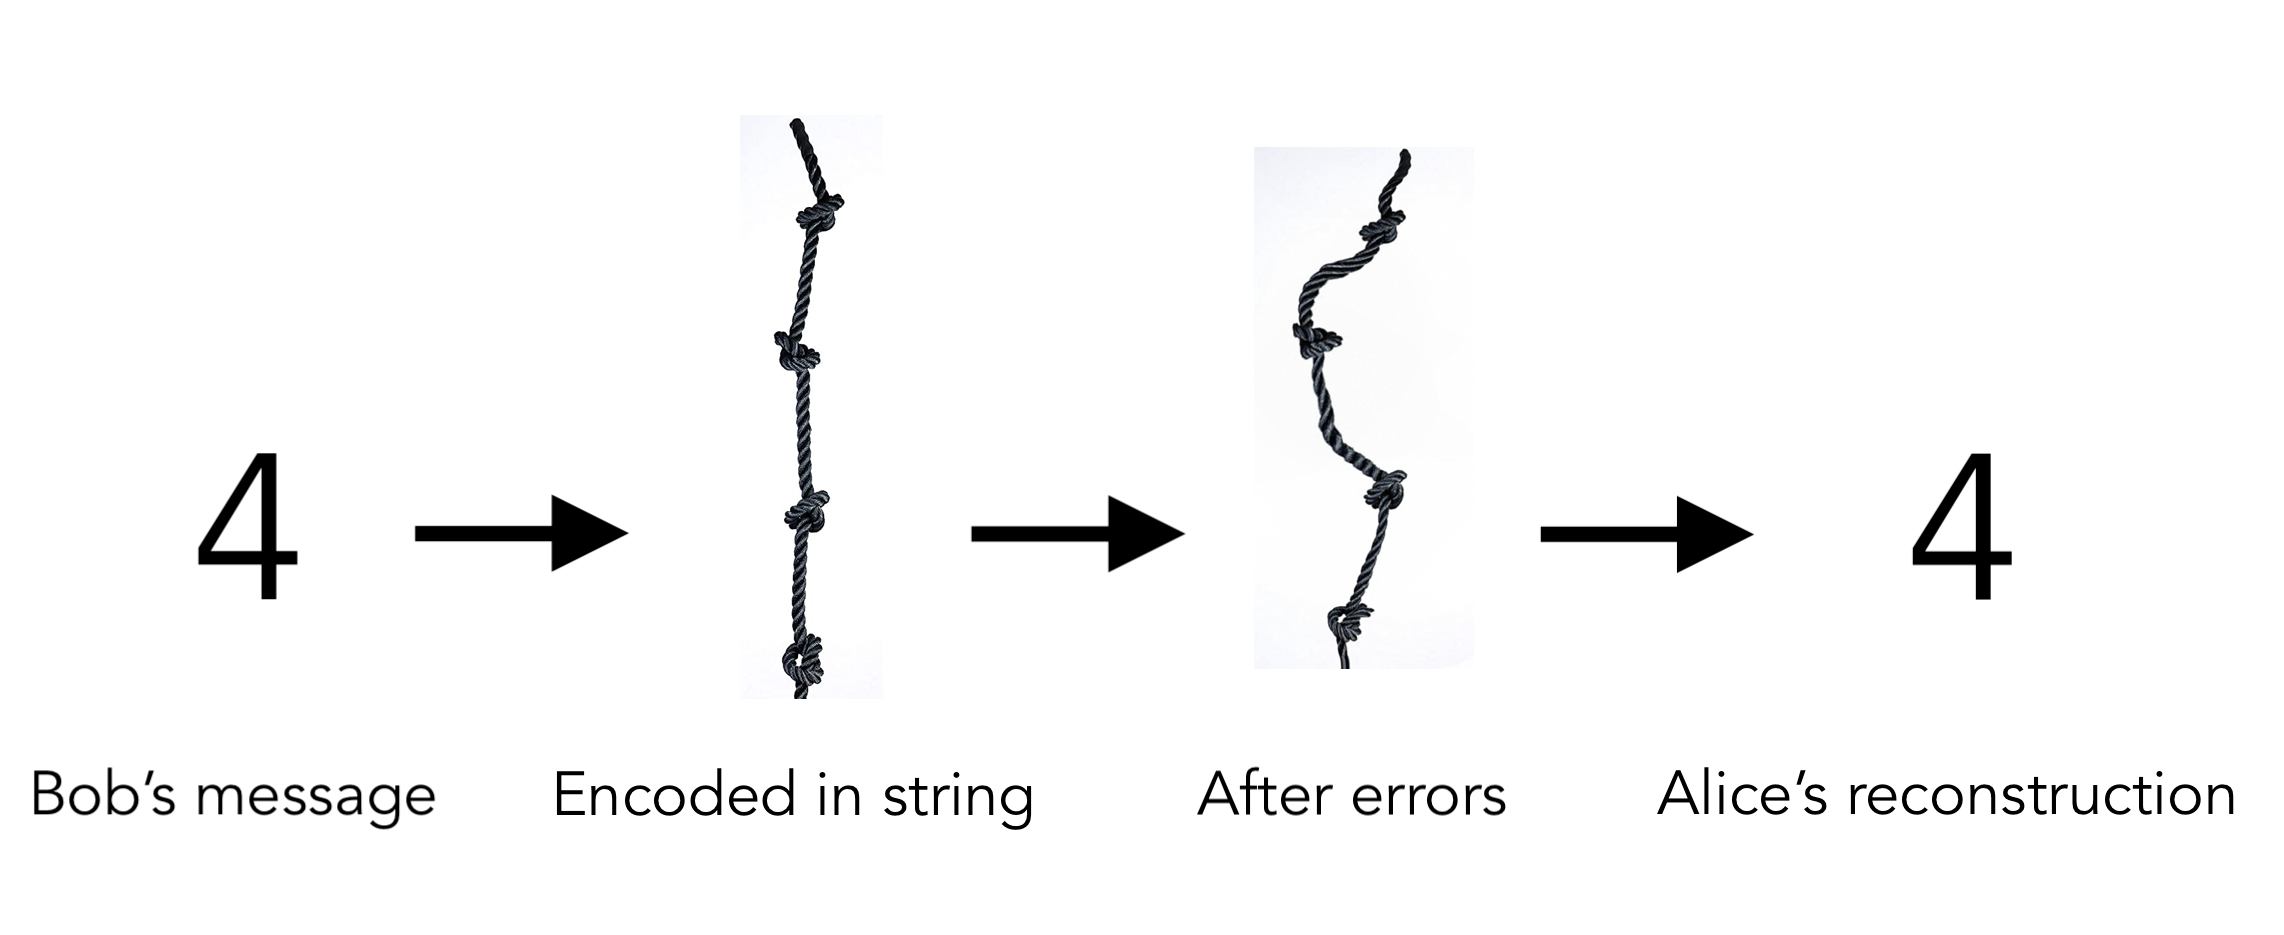
\includegraphics[scale=0.25]{rope-deformations}
\caption{A model of a (non-quantum) topological message}
\label{fig:rope-deformations}
\end{center}
\end{figure}

The answer is simple: Store the information in knots! By tying a certain number of simple knots in the string Alice can specify an integer that Bob can simply read off by counting (as in Figure \ref{fig:rope-deformations})! The beauty lies in the fact that while the string may be perturbed during the sending process, it would take a very specialized and unlikely error to untie the rope or to accidently re-tie an extra knot. This knotting number is a topological invariant (small perturbations don't change how many knots were tied), and so we can see intuitively that topological invariants are naturally error resistant.

The above situation is more than just a thought experiment: This is exactly the scheme that the ancient South American Incas used over 4000 years ago! The Incas stored all sorts of information in \textit{Quipus}, intricately knotted collections of fibered strings \cite{ascher1981code} as seen in Figure \ref{fig:quipu}. Storing information in knot invariants was also common practice in ancient Chinese, Tibetan, and Polynesian cultures \cite{day2021quipus}. In a sense, these are the earliest examples of topological computation.

\begin{figure}
\begin{center}
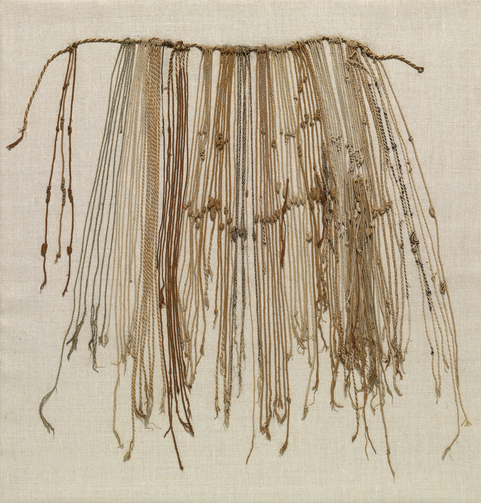
\includegraphics[scale=0.85]{quipu}
\caption{An Incan Quipu}
\label{fig:quipu}
\end{center}
\end{figure}

In TQC, information is still stored in knots. The main difference is that the strings being knotted are no longer physical pieces of twine, but \textit{trajectories of quasiparticles through spacetime}. For instance, suppose $X$ and $Z$ are two quasiparticles (we will elaborate more on this in later). Moving through space from time $t_0$ to $t_1$, the trajectories can look something like Figure \ref{fig:braiding}. Quantum interactions cause the knotting to yield real differences in physical states, and hence these knots can be used to store quantum information.

\begin{figure}
\begin{center}
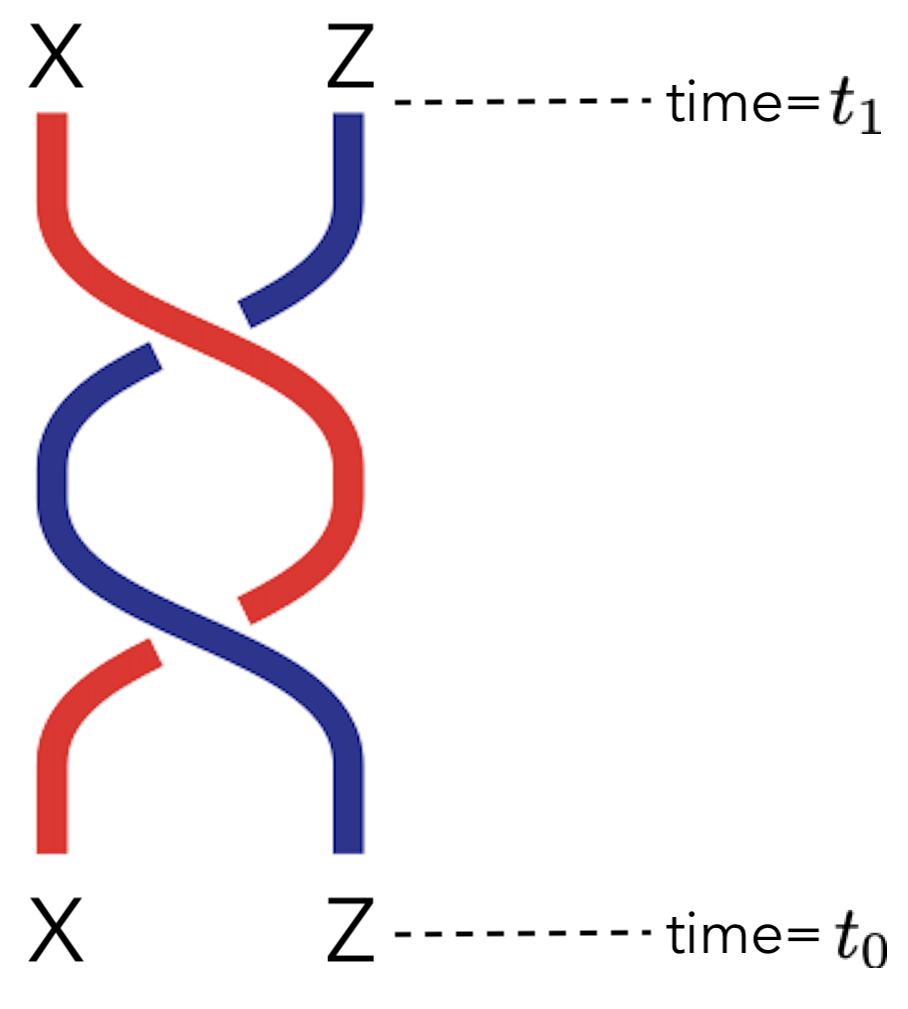
\includegraphics[scale=0.25]{braiding}
\caption{Braiding of quasiparticles in spacetime [WORK: do this in tikz]}
\label{fig:braiding}
\end{center}
\end{figure}

Notice that to make 3 dimensional spacetime, we modeled space as being 2 dimensional. While one might initially think this is a quirk of our human incapacity of visualizing 4 dimensional space, there is a deeper mathematical truth at play: There are no knots in 4 dimensional space. The extra dimension always gives the strands space to evade and move past each other without collision. In particular, for TQC to work we must have space be two dimensional. While this task seems initially impossible, phases of matter living entirely in a two dimensional subspace of our three dimensional world have been experimentally constructd\footnote{Of course, these are not \textit{literally} two dimensional. Motion in the third dimension is just so tightly constrained that $3$D models break down, and $2$D models start to work.}. Things that behave like particles in these 2 dimensional phases of matter are known as quasiparticles, and form non-trivial knots when braided.

The following is a rough description of how these 2 dimensional electron gasses are constructed. One begins by preparing a series of layers of graphene with a small gap in the middle. Upon subjecting the system to extremely cold temperatures and an extremely high magnetic field, the electrons in the graphene begin to move around. To balance the electric charge on both sides, all of the electrons move to the exact center of the setup. This resulting thin layer of electrons is a two dimensional electron gas. In such extreme conditions, all of the electrons will become highly entangled with each other, forming a quantum phase of matter \cite{yang2021experimental}. A diagram showing this process is found in Figure \ref{fig:spin-liquid}

\begin{figure}
\begin{center}
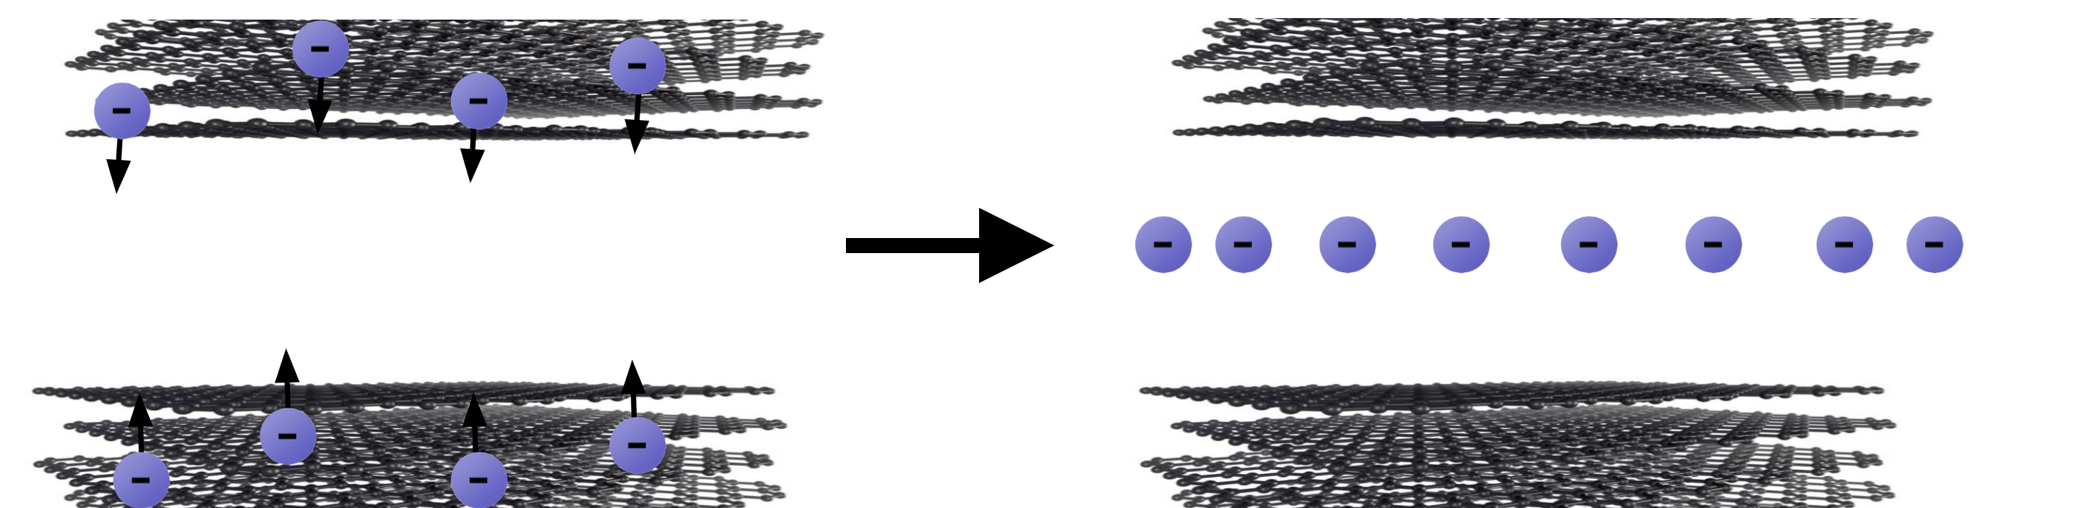
\includegraphics[scale=0.30]{spin-liquid}
\caption{The formation of an electron gas from graphene.}
\label{fig:spin-liquid}
\end{center}
\end{figure}

A key insight of Kitaev \cite{kitaev2003fault}, and one of the motivating pushes towards quantum computation, was that the topological properties of the 2 dimensional phase of matter will determine how the electrons entangled with each other. In other words, 2 dimensional sheets of electrons will form different quantum systems depending on their shape.

To understand this better, suppose that you have a 2 dimensional sphere of electrons. They will want to quantize, and align their spins together in the same direction. This amounts to choosing a unit tangent vector at each point on the sphere. However, there is no coherent way to do this. Every choice of tangent vectors will necessarily have some discontinuity or singularity: This is the content of the ``Hairy Ball Theorem".

If your sheet of electrons was on a donut, however, the situation is much different. There are several ways to coherently assign unit tangent vectors to each point; thus there are several ways for all of the electrons to quantize their spins together, as seen in Figure \ref{fig:hairy-ball}. This is aptly known as a \textit{spin liquid}. In mathematical language a ``donut" is called a torus, hence the name \textit{toric code}. The spin liquid associated with this procedure on a torus is called the ``$\ZZ_2$ spin liquid", and it is the physical realization of the toric code. We will spend the body of this manuscript describing the mathematics of the toric code in more detail. Note that generally when making such $\ZZ_2$ spin liquids in labs one does not make an actual torus; instead, one artificially simulates the boundary conditions of a torus in nanowires, for technical reasons \cite{albrecht2016exponential, mourik2012signatures}.

\begin{figure}
\begin{center}
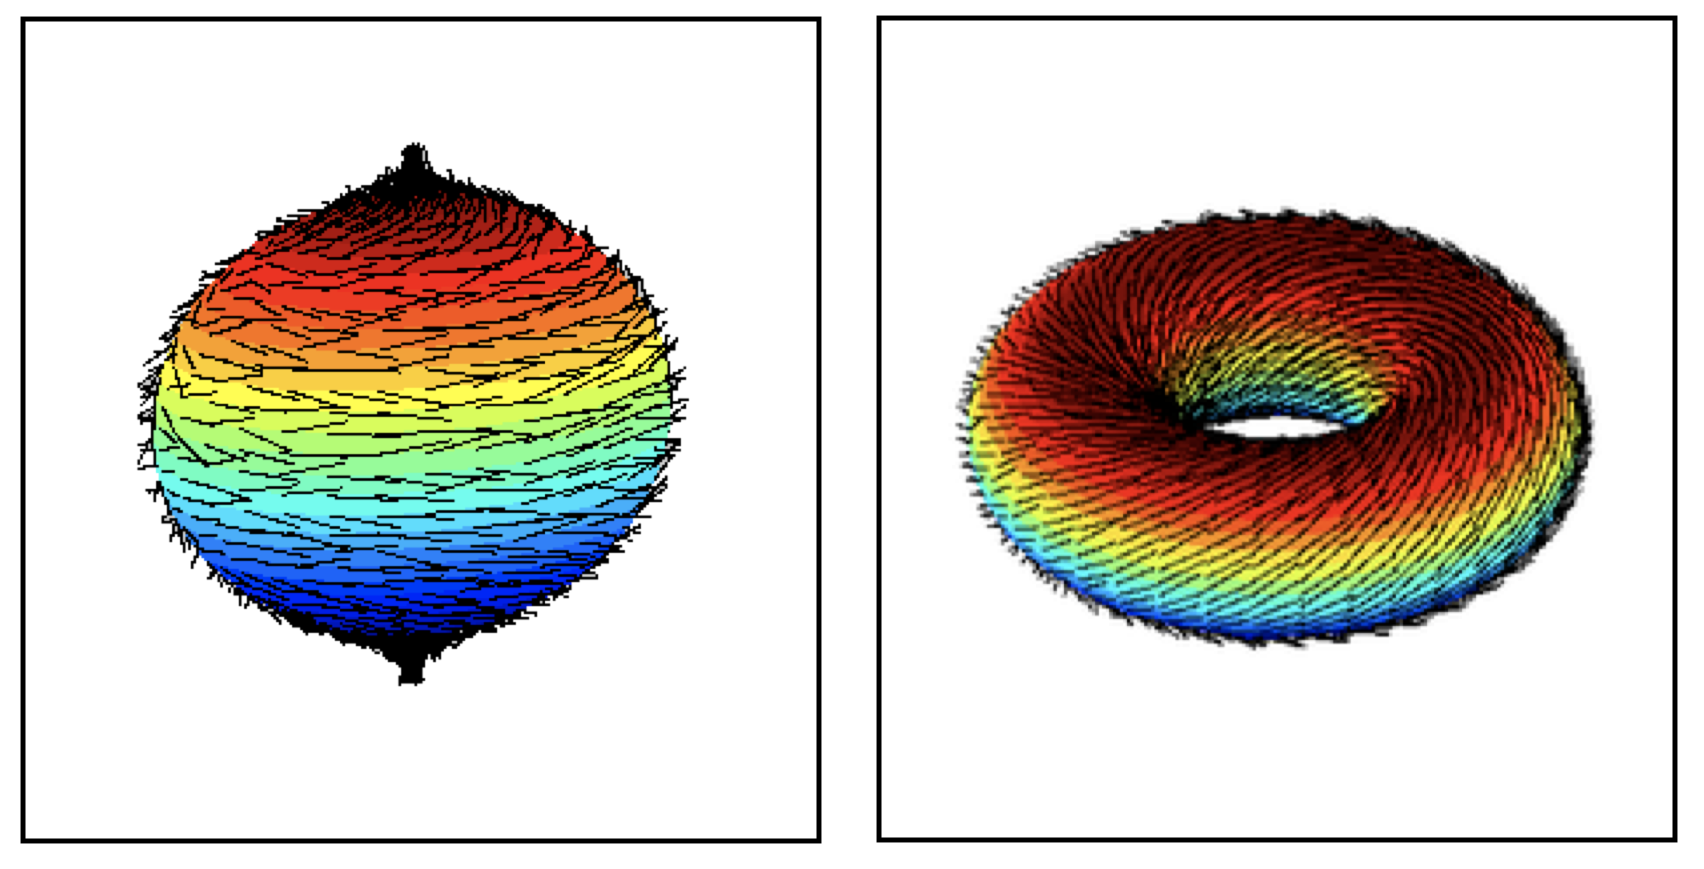
\includegraphics[scale=0.2]{Hairy-Ball-Diagram}
\caption{Assigning vector fields (spins) to a sphere, verses to a torus}
\label{fig:hairy-ball}
\end{center}
\end{figure}

We find it illustrative here to make an analogy with classical computing. Consider the following puzzle: Classical bits are stored in the magnetization of small regions on a hard disk. The magnetization of each atom is highly sensitive to thermal fluctuations. So why is it that classical computers seem so resistant to errors? The answer is that since all of the atoms are magnetized in the same direction, any one atom flipping will automatically be corrected back by the normalizing influence of the other atoms: magnets are naturally error resistant. It is exactly the same with these spin liquids that quantize together: Any one electron's spin decohering will immediately be corrected by the normalizing influence of all of its neighbors.

Before moving on to an in-depth treatment of the toric code, we offer a general description of the TQC process, in the style of the three points listed in the beginning of the introduction:

\begin{enumerate}
\item Information is stored in the ground states of topological quantum materials.
\item Ground states are acted on by braiding of quasiparticles, that is, by generating pairs of quasiparticles and knotting them in spacetime.
\item Measurements are performed by observing the topological properties of the resulting ground state.
\end{enumerate}

Here, \textit{ground state} refers to a state in the system with lowest possible energy. Note that in the previous description of spin liquids, all electrons having the same spin is a result of them being in the lowest energy state. An ``excited" electron with deviant spin will raise the energy of the system. These excited electrons are quasiparticles. In this way, quasiparticles can be interpreted as excitations of a topological quantum material. This motivates the fact that (topological) quantum computers must be exceptionally cold to function: Any extra energy will correspond to extra excitations, causing the computer to malfunction, since information is only stored in ground states.

The possibilities for topological quantum materials and TQC are extremely exciting, and we are eager to see where the field will go in the coming years.

\section{The Toric Code}
\label{The Toric Code}

Consider a torus. We will be imagining the torus as a whole as being a quantum system, corresponding physically to the quantum system one would observe when the torus is in the $\ZZ_2$ spin liquid topological quantum phase of matter. The \textit{code space} of the torus is the space of states on which we will be building our quantum computer, i.e., those states we will be using to store quantum information. In general Topological Quantum Computing (TQC) fashion, the code space of the toric code will be its ground states.

Our mathematical priorities are thus as follows: To define the quantum system, and to define a Hamiltonian operator on it. A Hamiltonian is an operator corresponding to the total energy of a quantum system. Namely, the eigenvalue of an eigenstate of the Hamiltonian corresponds to the total energy of that state. The code space will thus be the lowest eigenspace of the Hamiltonian.

\begin{figure}
\begin{center}
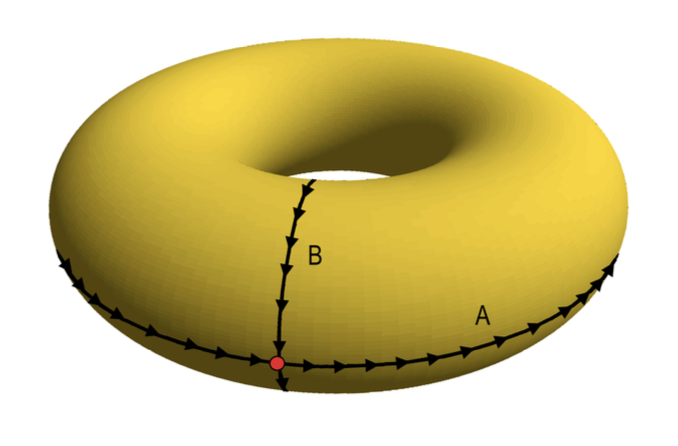
\includegraphics[scale=0.3]{torus}
\caption{Celluation of the torus, obtained by gluing opposite sides together.}
\label{fig:torus}
\end{center}
\end{figure}

Working with a continuous torus and the corresponding infinite dimensional vector spaces is cumbersome and unnecessary. Instead, we celluate the torus into an $n$ by $n$ square lattice with opposing sides identified, as in Figure \ref{fig:torus}. We will work with the understanding that the real physical system is the limit as $n\to\infty$. We define the quantum system associated with the $n$ by $n$ celluated torus to be the vector space

$$\Ncal=\bigotimes_{\substack{\text{edges of}\\\text{torus}}}\CC^2,$$

obtained by ``putting a qubit\footnote{A qubit is the quantum-computing term for ``two dimensional quantum system", i.e., $\CC^2$.}
on every edge". Here and throughout, \textit{vertices}, \textit{edges}, and \textit{faces}, when used as indexing sets, will refer to the set of \textit{vertices}, \textit{edges}, and \textit{faces} of our celluated torus. We will choose a canonical basis $\left\{\0,\1\right\}$ for $\CC^2$, reflecting our information theoretic intentions. To more forward with defining the Hamiltonian, we introduce the Pauli matrices

$$
\sigma_X=
\begin{pmatrix}
0 & 1\\
1 & 0
\end{pmatrix},\,\,
\sigma_Y=
\begin{pmatrix}
0 & -i\\
i & 0
\end{pmatrix},\,\,
\sigma_Z=
\begin{pmatrix}
-1 & 0\\
0 & 1
\end{pmatrix}.
$$

The Hamiltonian is defined by

$$H=-\sum_{\text{vertices } v}A_v-\sum_{\text{faces } p}B_p,$$

where

$$A_v=\bigotimes_{\substack{\text{edges}\\ \text{touching }v}}\sigma_Z,\,\, B_p=\bigotimes_{\substack{\text{edges}\\ \text{touching }p}}\sigma_X.$$

All of the power of the toric code comes from this highly non-obvious choice of Hamiltonian. The physical interpretation for this choice of Hamiltonian comes from gauge theory. Namely, the $U(1)$ Lattice Gauge Theory has two fields: The Compact Gauge Field and the Electric Field. Exponentiating the Compact Gauge Field we get the $\sigma_X$ operators, and exponentiating the Electric Field we get the $\sigma_Z$ operators. Thus, the $A_v$ contribute a ``Gauss' Law" term, and the $B_p$ contribute a ``Magnetic Field" term to the Hamiltonian \cite{oh2022rank}. While potentially physically illuminating, this discussion of gauge theory will have no influence on the rest of the mathematics presented in this manuscript, and does not need to be understood to appreciate the toric code.

Letting $I$ denote the identity matrix, the key facts about the $A_v$s and $B_p$s are summarized in the following proposition:

\begin{proposition}\label{AvBp}We have that

\begin{enumerate}[(i)]
\item $A_v^2=B_p^2=I$ for all $v,p$
\item All $A_v$s and $B_p$s have half eigenvalues $+1$ and half eigenvalues $-1$
\item All $A_v$s and $B_p$s commute
\item $\prod_{\text{vertices }v}A_v=I$ and $\prod_{\text{faces }p}B_p=I$
\end{enumerate}

\end{proposition}
\begin{proof}
$(i).$ Multiplying tensor product matrices corresponds to simply multiplying componentwise. Hence, this part  follows immediately from the relations $\sigma_X^2=\sigma_Z^2=I$.

$(ii).$ We define an isomorphism between the $+1$ eigenspace and $-1$ eigenspace of $A_v$. Namely, apply $\sigma_X$ to  an edge $e$ touching $v$. Since $\sigma_X\sigma_Z=-\sigma_Z\sigma_X$, the computation

$$A_v \left(\bigotimes_{\text{edge }e}\sigma_X\right)\ppsi = -A_v \left(\bigotimes_{\text{edge }e}\sigma_X\right)A_v\ppsi $$

show that a $+1$ eigenstate will be transformed into a $-1$ eigenstate, and a $-1$ eigenstate will be turned into $+1$ eigenstate. Thus, this defines an isomorphism between the desired eigenspaces. Applying $\sigma_Z$ instead of $\sigma_X$, we can define a similar isomorphism for $B_p$.

this will have the effect of turning a $+1$ eigenstate into a $-1$ eigenstate and vice-versa,

$(iii).$ All the $A_v$s commute with each other since $\sigma_Z$ commutes with itself, and all the $B_p$s commute with each other since $\sigma_X$ commutes with itself. What's left to check is that $A_vB_p=B_pA_v$. Notice that if $v$ is not touching the face $p$, none of the $\sigma_Z$s in the tensor product of $A_v$ will be in the same spots as any of the $\sigma_X$s as the tensor product for $B_p$. Hence, $A_v$ and $B_p$ commute in this case. If $v$ is touching $p$, then exactly two of the $\sigma_Z$s in the tensor product of $A_v$ will be in the same spots as $\sigma_X$s in the tensor product of $B_p$. Hence, pulling $B_v$ through $A_v$ corresponds to switching $\sigma_X$ and $\sigma_Z$. Since $\sigma_X\sigma_Z=-\sigma_Z\sigma_X$, this introduces an overall phase shift of $(-1)^2=1$. Hence, $A_vB_p=B_pA_v$ as desired!

$(iv).$ Applying $\prod_{\text{vertices } v}A_v$, is the same as applying $\sigma_Z$ to each vertex $2$ times, since each edge touches exactly $2$ vertices. Hence,

$$\prod_{\text{vertices } v}A_v=\bigotimes_{\text{edges}}\sigma^2_Z=\bigotimes_{\text{edges}}I=I.$$

Similarly, since every edge touches exactly $2$ faces, the fact that $\prod_{\text{faces } p}B_p=I$ follows from $\sigma^2_X=1$.
\end{proof}

Using the above facts about the $A_v$s and $B_p$s, we can describe the eigenspaces of $H$ well enough to compute their dimension:

\begin{proposition}\label{eigenspaces} All eigenvalues of $H$ are of the form $-2n^2+4q$, for an integer $q\leq n^2/2$. The $-2n^2+4q$ can be described as the space of states $\ppsi$ such that

$$\left|\left\{\left. v,p\right| A_v\ppsi =-1,\,\, B_p\ppsi=-1\right\}\right|=2q,$$

that is, the space of states with $2q$ excitations. There will always be an even number of $v$ such that $A_v\ppsi =-1$, as well as an even number of $p$ such that $B_p\ppsi=-1$. The dimension of of this eigenspace is

$$4\sum_{k=0}^{q}{n^2 \choose 2k} {n^2 \choose 2(q-k)}.$$

In particular, the code space of the toric code is 4 dimensional, and consists of those vectors $\ppsi$ such that $A_v\ppsi=B_p\ppsi=\ppsi$ for all $v,p$.
\end{proposition}
\begin{proof} To begin, we observe the following general fact from linear algebra. If $M$ and $N$ are commuting matrices and $\ppsi$ is an eigenvector for $N$ with eigenvalue $\lambda$, then

$$N(M\ppsi)=M(N\ppsi)=\lambda (M\ppsi).$$

Hence, $M$ respect the eigenspaces of $N$, and vice versa. This implies that the eigenspaces for $H$ will be simultaneous eigenspaces for all of the $A_v$s and $B_p$s, since all of the $A_v$s and $B_p$s commute by Proposition \ref{AvBp} (iii).

Suppose that $\ppsi$ is an eigenstate with

$$\left|\left\{\left. v,p\right| A_v\ppsi =-1,\,\, B_p\ppsi=-1\right\}\right|=q.$$

Then, we find that

\begin{align*}
H\ppsi&=(-\sum_{v}A_v-\sum_{p}B_p)\ppsi\\
&=\left(\sum_{\substack{v,p \\ -1\text{ eigenvalue}}}1-\sum_{\substack{v,p \\ 1\text{ eigenvalue}}}1\right)\ppsi\\
&=(q-(n^2-q))\\
&=-n^2+2q.
\end{align*}

Thus, to complete the initial description of the eigenstates, we must show that the number of $v$ such that $A_v\ppsi=-1$ and the number of $p$ such that $B_p\ppsi=-1$ is even. This follows from the computation that is this number where odd, then we would have by Proposition \ref{AvBp} (iv) that

$$\ppsi = \left(\prod_{v}A_v\right) \ppsi = -\ppsi,$$

which is a contradiction since we are supposing that $\ppsi\neq 0$. The exact same argument applies to the $B_p$. We now compute the dimensions of the eigenspaces. Let $D$ denote the dimension of the group space. We show that given any even sized sets $\bold{v}, \bold{p}$ of vertices and faces respectively, the space

$$\Ncal_{\bold{v},\bold{p}}=\{\left.\ppsi\right| \left(A_v\ppsi=-1\iff v\in \bold{v}\right),\,\, \left(B_p\ppsi=-1\iff p\in\bold{p}\right) \}$$

is $D$ dimensional. We proceed by induction on $|\bold{v}+\bold{p}|$. If $|\bold{v}+\bold{p}|=0$, then this is the definition of $D$. Without loss of generality, suppose $|\bold{v}|\geq 2$. If $|\bold{p}|\geq 2$, we apply the same arguement with verticies replaced by faces. Choose two verticies $v_0,v_1\in \bold{v}$. Choose a path $\gamma$ along the edges of the torus that connect $v_0$ and $v_1$. We show that $\bigotimes_{\text{edges in }\gamma}\sigma_X$ gives an isomorphism between $\Ncal_{\bold{v},\bold{p}}$ and $\Ncal_{\bold{v}-\{v_0,v_1\},\{p\}}$. Namely it is clear from $\sigma_X^2=\sigma_X$, so this map is its own inverse, so it is sufficient to show that the image is in the desired space. To prove this, we observe that $\bigotimes_{\text{edges in }\gamma}\sigma_X$ commutes with all the $B_p$s, and commutes with all of the $A_v$s at verticies that $\gamma$ passes through an even number of times. The only verticies that $\gamma$ passes through an odd number of times are its endpoints (by definition), and hence $A_v$ has exactly the effect of flipping the eigenvalues at $A_{v_0}$ and $A_{v_1}$. Thus, the image of a point in $\Ncal_{\bold{v},\bold{p}}$ is in $\Ncal_{\bold{v}-\{v_0,v_1\},\bold{p}}$, as desired.

Combining, we find that the $-2n^2+2q'$ eigenstate can be decomposed as direct sums of $\Ncal_{\bold{v},\bold{p}}$, where $\bold{v}$ and $\bold{p}$ range over even sized sets with $|\bold{v}+\bold{p}|=q'$. In particular, $q'=2q$ must be even. The dimension of this space is equal to $D$ times the number of way of choosing the sets $\bold{v}$ and $\bold{q}$, i.e.,

$$D\sum_{k=0}^{q}{n^2 \choose 2k}{n^2 \choose 2(q-k)}.$$

The total dimension of eigenspaces of $H$ can be computed as

\begin{align*}
D\sum_{q=0}^{2n^2}\sum_{k=0}^{q}{n^2 \choose 2k}{n^2 \choose 2(q-k)}&=D\left(\sum_{q=0}^{2n^2}{n^2 \choose 2k_0}\right)\\
&=D\cdot \left(2^{n^2-1}\right)^2=D\cdot 2^{2n^2-2}.
\end{align*}

The Hamiltonian is a symmetric matrix with real coefficients, since it is the tensor product of such matrices. It is a standard fact from linear algebra that such matrices can be diagonalized, and hence the total dimension $H$ is equal to the dimension of $\Ncal=\bigotimes_{\text{edges}}\CC^2$. Seeing as there are $2n^2$ edges this space is $2^{2n^2}$ dimensional, and hence we must have $D=2^2=4$.
\end{proof}

The fact that the code space is four dimensional can be motivated as follows. By Proposition \ref{AvBp} (ii), being in the $+1$ eigenspace for each $A_v$ and $B_p$ will impose a condition that decreases the dimension of your space by $1/2$. Since $\Ncal$ is $2^{2n^2}$ dimensional, imposing all $n^2$ of these conditions decreases the code space to $1$ dimension. However, the fact that $\prod_{\text{vertices }v}A_v=I$ and $\prod_{\text{faces }p}B_p=1$  from Proposition \ref{AvBp} (iv) shows that two of these conditions imposed were redundant, brining the code space dimension back up to $2^2=4$ dimensions.

To describe the generators of the codespace explicitly we will need to use the basics of homology theory with $\ZZ_2$ coefficients, where $\ZZ_2=\{0,1\}$ is the additive group modulo $2$. For those unfamiliar, a brief introduction is included in Appendix \ref{Homology}.

\begin{figure}
\begin{center}
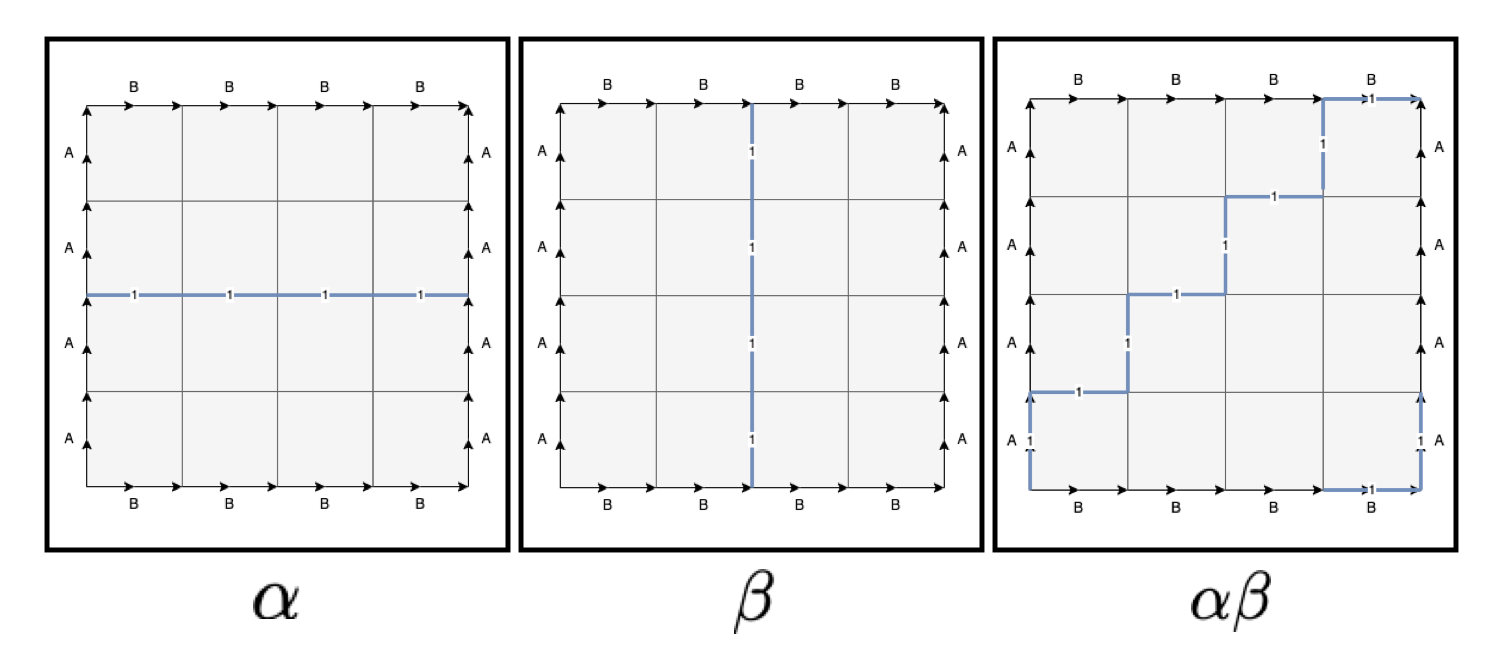
\includegraphics[scale=0.35]{homology-classes}
\caption{The three non-trivial homology classes of a torus}
\label{fig:homology}
\end{center}
\end{figure}


A pure state on $\Ncal$ is specified by a pure state on each qubit, namely, a choice of $\0$ and $\1$ for each edge. This is exactly the data to specify a $\ZZ_2$-chain. Given a $\ZZ_2$-chain $\gamma$, we write $\left|\gamma\right>$ for the associated pure state. Given any $\gamma,\gamma'$, we write $\gamma\sim \gamma'$ to mean that $\gamma$ and $\gamma'$ are homologous. The following elucidates the meaning of the codespace of the toric code:

\begin{proposition}\label{basis} Let $\bold{0},\alpha,\beta,$ and $\alpha\beta$ be the four $\ZZ_2$ homology classes on the torus, as in Figure \ref{fig:homology}. Choose $\bold{0}_0$, $\alpha_0$, $\beta_0$, and $(\alpha\beta)_0$ respectively to be representatives. Then, letting $\gamma$ run over all $\ZZ_2$-cycles, we have that

\begin{align*}
\nullclass &= \frac{1}{\sqrt{2^{n^2-1}}}\sum_{\gamma\sim \bold{0}_0}\left|\gamma\right>,\,\, \alphaclass=\frac{1}{\sqrt{2^{n^2-1}}}\sum_{\gamma\sim \alpha_0}\left|\gamma\right>,\\
\betaclass &= \frac{1}{\sqrt{2^{n^2-1}}}\sum_{\gamma\sim \beta_0}\left|\gamma\right>,\,\, \alphabetaclass=\frac{1}{\sqrt{2^{n^2-1}}}\sum_{\gamma\sim (\alpha\beta)_0}\left|\gamma\right>,
\end{align*}

are all normalized eigenstates of that Hamiltonian $H$, and serve as a canonical orthonormal basis of the codespace.
\end{proposition}
\begin{proof} Choose $\omega\in H_1(T;\ZZ_2)$. To show that $\left|\omega\right>$ is in the codespace, we observe that it is in the $+1$ eigenspace of every $A_v$ and $B_p$. Since $\sigma_Z$ sends $\0$ to $\0$ and $\1$ to $-\1$, $A_v$ has the effect of sending a pure state $\left|\gamma\right>$ to $\pm\left|\gamma\right>$, depending on whether $\gamma$ has an odd or even count of edges touching the vertex $v$. In particular, because $\gamma$ is running over cycles, we have that each $\left|\gamma\right>$ is in the $+1$ eigenspace of all the $A_v$, and hence the same applies to $\left|\omega\right>$.

For $B_p$s, we observe that applying $B_p$ to a pure state $\left|\gamma\right>$ has the effect of flipping all of the qubits around the face $p$. By definition of being $\ZZ_2$ homologous, $B_p$ maps the space of all cycles homologous to $\left|\omega\right>$ back into the space of all cycles homologous to $\left|\omega\right>$. In particular, $\left|\omega\right>$ is in the $+1$ eigenspace of $B_p$ for every $p$.

To show that $\left|\omega\right>$ is normalized, we observe that there are exactly that there are exactly $2^{n^2-1}$ cycles homologous to $\omega$. This is proved as follows. Starting with a fixed representative $\omega_0$ of $\omega$, cycles homologous to $\omega$ correspond to flipping qubits around the edges, i.e., applying $B_p$s at faces. Since there are $n^2$ faces, this gives $2^{n^2}$ cycles. This overcounts the space of cycles homologous to $\omega$ by a factor of $2$, since $\prod_{\text{faces }p}B_p=I$ by Proposition \ref{AvBp} (iv). The fact that the codespace is 4 dimensional says that this is the \textit{only} relation between the $B_p$s. Hence, there are $2^{n^2-1}$ cycles.

To show that these states are mutually orthogonal, we observe simply that no cycle can be homologous to two of the $\{\bold{0},\alpha,\beta,\alpha\beta\}$, hence $\left\{\nullclass,\alphaclass,\betaclass,\alphabetaclass\right\}$ have disjoint support, hence they are orthogonal.
\end{proof}

Letting $T$ denote the torus, the above shows that we can view the codespace of the toric code as a physical realization of the vector space $\CC[H_1(T;\ZZ_2)]$. Here, $\CC[A]$ for some set $A$ denotes the vector space generated by $A$, i.e., the unique complex vector space which has a basis given by $A$. Quantum physics gives the physical analogue of the abstract mathematical notation of an equivalence class, namely, an equivalence class is realized as the superposition over all possible representatives. This can be compared with the path integral formulation of quantum mechanics, where one integrates over all possible paths between two points.

We now give \textit{quasiparticle} interpretation of the toric code. A quasiparticle is an excitation in the toric code. Namely, given an eigenstate $\ppsi$, we say that there is a quasiparticle at a vertex $v$ if $A_v\ppsi=-\ppsi$, and get a face $p$ we say that there is a quasiparticle at $p$ if $B_p\ppsi=-\ppsi$.

Let $\ppsi$ be an eigenstate, and let $v_0,v_1$ be adjacent vertices connected by an edge $e$. Suppose that there is a quasiparticle at $v_0$, and that there is not a quasiparticle at $v_1$. Let $\left| \psi'\right>$ be the state obtained by applying $\sigma_X$ to the edge $e$. We observe that

$$A_{v_0}\left| \psi'\right> = A_{v_0}\left(\bigotimes_{\text{edge }e}\sigma_X\right)\ppsi=-A_{v_0}\ppsi=\ppsi,$$

$$A_{v_1}\left| \psi'\right> = A_{v_1}\left(\bigotimes_{\text{edge }e}\sigma_X\right)\ppsi=-A_{v_1}\ppsi=-\ppsi,$$

where we used the key fact that $\sigma_X\sigma_Z=-\sigma_Z\sigma_X$. Additionally, $A_{v}\left|\psi'\right>=A_{v}\ppsi$ for $v\neq v_0,v_1$, since applying $\sigma_X$ to $e$ only affects the verticies $v_0$ and $v_1$. We can interpret this computation as saying the following: Applying $\sigma_X$ has the effect of \textit{moving the quasiparticle along e}, from $v_0$ to $v_1$. Applying longer chains of $\sigma_X$s, we see in general that applying $\sigma_X$ corresponds to moving quasiparticles at verticies along the edges. If neither $v_0$ nor $v_1$ had quasiparticles, then again tensoring with $\sigma_X$ at $e$ would have the effect of flipping the eigenvalues at $v_0$ and $v_1$, i.e., the effect of \textit{creating quasiparticles at the endpoints of e}, at $v_0$ and $v_1$. If both $v_1$ and $v_1$ has quasiparticles, then tensoring with $\sigma_X$ at $e$ would have the effect of \textit{anhilating quasiparticles at the endpoints of e}.

In summary, the quasiparticles at edges are their own antiparticle. Creating particle/antiparticle pairs, moving the quasiparticles, and annihilating particle/antiparticle pairs all are mathematically realized by the simple operation of tensoring edges with $\sigma_X$.

Similarly, we can describe the quasiparticles sitting at faces, corresponding to faces with an excitation $B_p\ppsi=-\ppsi$. Tensoring with $\sigma_X$ has no effect on these quasiparticles, since tensoring with $\sigma_X$ at any edge commutes with all the $B_p$: $\sigma_X$ commutes with itself. However, it is now tensoring with $\sigma_Z$ that causes the motion of particles. Given faces $p_0,p_1$ with common edge $e$, tensoring with $\sigma_Z$ at $e$ has the effect of moving a quasiparticle from $p_0$ to $p_1$ if exactly one of the faces had a quasiparticle, has the effect of creating a particle/antiparticle pair if neither of the faces has quasiparticles, and has the effect of annihilating a particle/antiparticle pair if both faces have quasiparticles.

Summarizing, we find that the toric code naturally have two types of quasiparticles, an $X$-type that lives on vertices which moves by tensoring by $\sigma_X$, and a $Z$-type that lives in faces and moves by tensoring with $\sigma_Z$. This allows us to mathematically implement a topological quantum computer. Namely:

\begin{enumerate}
\item Quantum information is stored in the ground state of the toric code, i.e., the lowest eigenvalue eigenspace of the Hamiltonian.
\item Ground states are acted on by generating and manipulating quasiparticles, moving them around the torus, and annihilating them. Mathematically, this is realized by repeatedly tensoring with $\sigma_X$ and $\sigma_Z$ along edges, until one returns to a ground state.
\item Quantum information is measured by observing the ground state with respect to the canonical orthonormal basis of the codespace, given in Proposition \ref{basis}
\end{enumerate}


As an example, we implement the ``$\text{NOT}_\alpha$" gate, which flips the input state depending on whether it has an $\alpha$ component, namely

\begin{align*}
&\nullclass \mapsto \alphaclass,\,\,  \betaclass \mapsto \alphabetaclass \\
&\alphaclass \mapsto \nullclass,\,\, \alphabetaclass \mapsto \betaclass.
\end{align*}

\begin{figure}
\begin{center}
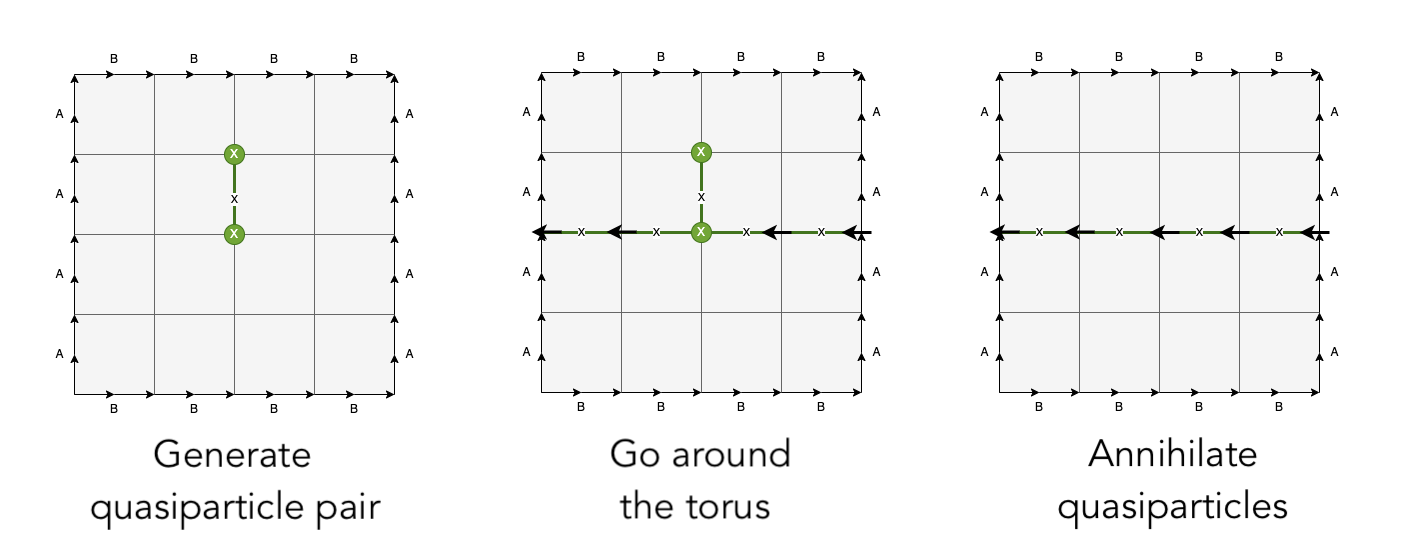
\includegraphics[scale=0.45]{not-alpha-gate}
\caption{Topological quantum process implementing the $\text{NOT}_{\alpha}$ gate}
\label{fig:not-alpha-gate}
\end{center}
\end{figure}

A diagram visualizing the process described in the following proposition is shown in Figure \ref{fig:not-alpha-gate}.

\begin{proposition} The following computation has the effect of performing the $\text{NOT}_{\alpha}$ gate. First, generate a particle/antiparticle pair of $X$-type particles. Then, move one of the particles around the torus via a path homologous to $\alpha$. Finally, fuse your two adjacent $X$-type particles together.
\end{proposition}
\begin{proof} Let $v_0$ and $v_1$ be adjacent vertices. Let $\alpha_0$ be a cycle homologous to $\alpha$ going from $v_1$ to itself. The process described in the statement of the proposition can be reworded as saying the following. First, we create a particle pair at $v_0$ and $v_1$, i.e., we tensor with $\sigma_X$ at the edge connecting $v_0$ and $v_1$. Then we move $v_1$ along $\alpha_0$, i.e., we tensor with $\sigma_X$ along the edges in $\alpha_0$. Then, we fuse the $X$-type quasiparticles at $v_0$ and $v_1$ back together, i.e., we tensor along the edge connecting $v_0$ and $v_1$ again. Since $\sigma_X^2=1$, this whole process can be described mathematically as

$$\bigotimes_{\text{edges in }\alpha_0}\sigma_X.$$

Seeing as $\sigma_X$s corresponds to flipping $\0$s to $\1$s in pure states, this process has the effect of flipping all of the qubits along $\alpha_0$. On the level of cycles, this means that we take $\left|\gamma\right>$ to $\left|\gamma+\alpha_0\right>$, where addition is in the group of cycles. Seeing as adding a cycle homologous to $\alpha$ to a cycle homologous to $\omega$ results in a cycle homologous to $\omega+\alpha$ we find thus that this process has the effect of sending $\left|\omega\right>$ to $\left|\omega+\alpha\right>$. Seeing as $\alpha+\alpha=0$ in $H_1(T;\ZZ_2)$, this process is exactly the $\text{NOT}_{\alpha}$ gate.
\end{proof}

Similarly, we can implement the $``(-1)_{\alpha}"$ gate, which flips the input state depending on whether it has an $\alpha$ component, namely

\begin{align*}
&\nullclass \mapsto \nullclass,\,\,  \betaclass \mapsto \betaclass \\
&\alphaclass \mapsto -\alphaclass,\,\, \alphabetaclass \mapsto -\alphabetaclass.
\end{align*}

\begin{proposition}\label{Xparticle} The following computation has the effect of performing the $\text{(-1)}_{\alpha}$ gate. First, generate a particle/antiparticle pair of $Z$-type particles. Then, move one of the particles around the torus via a path homologous to $\beta$. Finally, fuse your two adjacent $Z$-type particles together.
\end{proposition}
\begin{proof} Let $p_0$ and $p_1$ be adjacent faces. Let $\beta_0$ be a cycle homologous to $\beta$ going from $p_1$ to itself. Note that since $Z$-type particles live on faces, $\beta_0$ does not consist of a series of edges. Instead, it is a path going through the centers of faces. We take $\widehat{\beta}_0$ to be the set of edges that $\beta_0$ passes through. Tensoring with $\sigma_Z$ along $\widehat{\beta}_0$ corresponds to motion of a particle from $p_1$ along $\beta_0$ back to itself.

\begin{figure}
\begin{center}
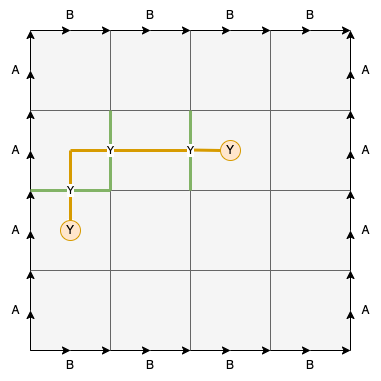
\includegraphics[scale=0.30]{dual-celluation}
\caption{Sample trajectory along dual celluation of torus}
\label{fig:dual-celluation}
\end{center}
\end{figure}

These cycles that go through faces of the torus are called \textit{dual cycles}, and are standard practice in the theory of homology. Namely, they are cycles in the dual celluation, as seen in Figure \ref{fig:dual-celluation}. Whereas the edges associated with a normal cycle satisfy the property `every vertex touches an even number of $1$s', the edges associated with a cycle in the dual celluation satisfy the dual condition `every face touches an even number of $1$s'.

As before, we find that the whole process can be described mathematically as

$$\bigotimes_{\text{edges in }\widehat{\beta}_0}\sigma_Z.$$

The matrix $\sigma_Z$ acts on pure states by sending $\0$ to itself, and $\1$ to $-\1$. Thus, this process has the effect of introducing a $-1$ global phase shift for every $1$ in states along $\widehat{\beta}_0$. Thus, when acting on a pure state $\gamma$, the definition of $\widehat{\beta}_0$ shows that this process has the effect of introduce a phase shift of $-1$ to the power of the number of intersection between $\gamma$ and $\widehat{\beta}_0$.

It is a well known fact that this signed intersection number ($-1$ to the power of the number of intersections) is an invariant in $\ZZ_2$ homology. To see this, observe that changing representatives of a homology class correspond to flipping qubits around a face. By the `dual cycle' condition, this flipped face will touch an even number of elements in the dual cycle. Hence, the intersection number will change by an even amount, leaving $-1$ to the power of that number invariant.

In particular, $\bold{0}$ doesn't intersect $\beta$, $\beta$ doesn't intersect $\beta$ (representatives can be chosen to be parallel), $\alpha$ intersects $\beta$ (horizontal loops and vertical loops meet at exactly one point), and $\alpha\beta$ intersects $\beta$. Thus, this process has the effect of adding a $-1$ phase shift to those states which include an `$\alpha$', as desired.
\end{proof}

Sadly for the toric codes, these are essentially the only gates that can be implemented. No matter how one moves around particles, there is not enough complexity in the system to generate interesting gates. We formalize this by writing out the \textit{group of gates} of the toric codes. We can think of quantum gates on a system as forming a group, where the group law is given by the composition of gates, and every element has an inverse since unitary matrices are invertible. For the toric codes, we have the following:

\begin{proposition}\label{Yparticle} There are exactly 8 possible computations in the toric codes. The group of gates is (non canonically) isomorphic to the Pauli group, i.e., the group whose objects are

$$\{\pm I, \pm iI, \pm \sigma_X, \pm i \sigma_X, \pm \sigma_Y, \pm i\sigma_Y, \pm \sigma_Z, \pm i \sigma_Z\}$$

and whose group operation is given by matrix multiplication. A minimal generating set is given by $\{\text{NOT}_{\alpha},\text{NOT}_{\beta},(-1)_{\alpha}\}$.
\end{proposition}
\begin{proof} To begin, we define $\text{NOT}_{\beta},\text{NOT}_{\alpha\beta},(-1)_{\beta},$ and $(-1)_{\alpha\beta}$ in complete analogy to how we define $\text{NOT}_{\alpha}$ and $(-1)_{\alpha}$. Namely, $\text{NOT}_{\beta}$ flips whether or not a state has a `$\beta$' in it, and $\text{NOT}_{\alpha\beta}$ flips whether or not a state has an `$\alpha\beta$' in it, i.e.,

\begin{align*}
&\nullclass \mapsto \alphabetaclass,\,\,  \betaclass \mapsto \alphaclass \\
&\alphaclass \mapsto \betaclass,\,\, \alphabetaclass \mapsto \nullclass.
\end{align*}

The relation $\sigma_X\sigma_Z=-\sigma_Z\sigma_X$ implies that we can switch the order of operations between first applying all our $\sigma_X$s and then applying all our $\sigma_Z$s, up to an operator-wise phase shift $-1$. Any process of creating and annihilating $X$-type quasiparticles can be modeled in sequence as repeatedly creating particles, moving them around a loop, then annihilating them. Following the proof of Proposition \ref{Xparticle}, this is the same as repeatedly applying $\text{NOT}_{\omega}$ gates, for homology classes $\omega$. Similarly, the processes on $Z$-type particles will be compositions of $(-1)_{\omega}$ gates.

Hence, we now have a full set of generators for our gate group: $\{\pm I, \text{NOT}_{\omega}, (-1)_{\omega}\}$, where $\omega$ runs over homology classes. The relations $\text{NOT}_{\alpha}\text{NOT}_{\beta}=\text{NOT}_{\alpha\beta}$ and $(-1)_{\alpha}(-1)_{\beta}=(-1)_{\alpha\beta}$ allow one to reduce the generating set further. The relations

$$\text{NOT}_{\alpha}(-1)_{\alpha}\text{NOT}_{\alpha}=(-1)_{\beta}$$

and

$$(-1)_{\alpha}\text{NOT}_{\alpha}(-1)_{\alpha}=-I$$

reduce the generating set to $\{\text{NOT}_{\alpha},\text{NOT}_{\beta},(-1)_{\alpha}\}$. Verifying simple relations gates, it is simple to see that the gate group is isomorphic to the Pauli group, as desired.


\end{proof}


Before moving on to the next section, we make a few final remarks about the behavior of quasiparticles on the toric codes. Namely, we observe the following. Consider the full vector space $\Ncal$, and adjacent two adjacent $X$-type and $Z$-type quasiparticles. Consider the simple braiding of these particles around each other, as in Figure \ref{fig:braiding}. A line going under another corresponds to the particle having passed through that space first, before the other particle. This braiding can be obtained by first performing a twist halfway around the circle by $X$, then a twist all the way around the circle by $Z$, then finally moving the second half of the circle by $X$. This process corresponds to a transformation $\Ncal\to \Ncal$ (i.e. tensoring with the appropriate $\sigma_X$s and $\sigma_Z$s). The observation is that this transformation is \textit{not} the identity on the codespace. Namely, since $\sigma_Z\sigma_X=-\sigma_X\sigma_Z$, this operation corresponds to a global phase shift of $-1$ on the system.

Thus, the braiding of $X$ type and $Z$ type particles corresponds to a phase shift of $-1$. This is in contrast to braiding two identical $X$ type or $Z$ type particles, which corresponds to the identity since $\sigma_X$ and $\sigma_Z$ commute with themselves. All particles in the standard model of physics are \textit{fermions}, which give a phase shift of $-1$ when you braid them with themselves, or \textit{bosons}, which act by the identity when you braid them with themselves. Seeing as $X$ type and $Z$ type particles in the toric code braid by the identity with themselves, one would expect them to be bosons. However, bosons always braid by the identity with each other and hence the $-1$ phase shift from braiding $X$ and $Z$ type particles should be impossible. The conclusion is that these really are \textit{quasi}particles, which behave much differently than particles in the standard model. Quasiparticles with simultaneously non-bosonic and non-fermionic braiding rules are known as \textit{anyons}. The name comes from the fact that they can have ``any " braiding rules, hence ``any"-on.  All interesting particles in topological quantum phases of matter will be anyons.

In the case of the toric code, the braiding will always be trivial or give a global phase shift (i.e. -1). We call anyons \textit{non-abelian} if they can braid in such a way to create transformations that are not phase shifts. To  create interesting quantum gates, these sort of non-phase shift braidings are what we need. The search for a topological quantum computer is essentially the search for experimentally-sound easy-to-braid non-abelian anyons.

$\newline\newline$

\large \textbf{Exercises}:\normalsize

\begin{enumerate}[\thesection .1.]
\item For edges $v$ and faces $p$, define

$$A_v'=\bigotimes_{\substack{\text{edges} \\ \text{touching }v}}\sigma_X,\,\, B_p'=\bigotimes_{\substack{\text{edges} \\ \text{touching }p}}\sigma_Z,$$

$$H'=-\sum_{\text{vertices }v}A_v'-\sum_{\text{faces }p}B_p'.$$

Let $M=\frac{1}{\sqrt{2}}
\begin{pmatrix}
1 & 1 \\
1 & -1
\end{pmatrix}$ be the Hadamard matrix. Using the relations

$$\sigma_X=M\sigma_ZM^{-1},\,\, \sigma_{Z}=M\sigma_X M^{-1},$$

show that $H$ and $H'$ are similar, in the sense that $H'=MHM^{-1}$. Use this to conclude that all basis independent properties of the toric code are formally symmetric by replacing $X$ with $Z$. In particular, the codespace (lowest eigenspace) of $H'$ is 4 dimensional, and the gate group of $H'$.


\item Show that eigenvectors of the Hamiltonian are equally likely to give $0$ or $1$ when measured at every qubit. This implies that the eigenvectors of the Hamiltonian are \textit{maximally entangled}, which is a more general phenomenon in TQC. (HINT: Prove this for ground states first, then lift to general eigenstates using an induction argument along the lines of the proof of Proposition \ref{eigenspaces})

\item Let $\Ncal_{n}$ denote the vector space associated to the $n$ by $n$ grid on the torus. Let

$$\tilde{H}_n=H_n+(2n^2)I,$$

so that the ground states have eigenvalue $0$. This is more physically realistic, since systems cannot have negative energy. When $n$ divides $m$, we have a natural map

$$\Ncal_{n}\hookrightarrow{}\Ncal_{m}$$

defined by [WORK: What is the correct definition?]. Show that this map is linear and injective, and hence that $\Ncal_{n}$ can be realized as a sub vector space of $\Ncal_{m}$. Show that $\tilde{H}_{m}$ restricted to $\Ncal_{n}$ is equal to $\tilde{H}_n$. Show that the map $\Ncal_{n}\hookrightarrow{}\Ncal_{m}$ is norm-preserving, in the sense that if $\left|\chi\right>,\left|\psi\right>$ are states on $\Ncal_{n}$, the inner product $\left<\chi | \psi \right>$ is independent of whether or not it was computed in $\Ncal_{n}$ or $\Ncal_{m}$. Define

$$\Ncal_{\infty}=\bigcup_{n=3}^{\infty}\Ncal_{n},$$

and define $\tilde{H}_{\infty}$ to be the operator on $\Ncal_{\infty}$ which acts on vectors in $\Ncal_{n}$ by $\tilde{H}_n$. Show that these are well defined objects, that $\Ncal_{\infty}$ is naturally a Hilbert space. It is in this sense that we can speak of a limiting continuous model formed by the discrete grid celluations\footnote{Note that objects in $\Ncal_{\infty}$ themselves aren't continuous paths; they are just discrete cycles in $\Ncal_n$ for some $n$. This is not an issue, since the \textit{simplicial approximation theorem} says that every continuous phenomenon can be modeled discreetly in a fine enough celluation.}.
\end{enumerate}

\section{Topological Quantum Field Theories}
\label{TQFTs}

\subsection{The general picture}
\label{The general picture}

Topological Quantum Computation (TQC) is physically based on topological quantum phases of matter. Topological Quantum Field Theories are the mathematical formalism of topological quantum phases of matter. Namely, every topological quantum phase of matter (physical object) has an associated Topological Quantum Field Theory (mathematical object) to describe it. To make this clearer, we recall classical phases of matter in a more mathematical way. Namely, a phase of matter is an assignment

$$
\begin{pmatrix}
\text{Collections of } \\
\text{particles}
\end{pmatrix}
\bigleadsto
\begin{pmatrix}
\text{Physical\,} \\ \text{systems}
\end{pmatrix},
$$

taking a set of particles to the way it would behave under the phase of matter. The ``gas" phase of matter will take a collection of particles and make the physical system of having them all bounce around each other really fast. The ``solid" phase of matter will take that same collection of particles and have them move less freely, forming a more crystalline structure. A quantum phase of matter should do the exact same thing, but now your physical system is replaced by a quantum system. Namely, a quantum phase of matter is an assignment

$$
\begin{pmatrix}
\text{Collections of } \\
\text{particles}
\end{pmatrix}
\bigleadsto
\begin{pmatrix}
\text{Quantum\,} \\ \text{systems}
\end{pmatrix}.
$$

Topological quantum phases of matter arise from the understanding that the topology of a shape (i.e. the physical invariants of the shape invariant under deformation) will affect the quantum system arising from inducing that shape with a given phase of matter. For example, consider the ``$\ZZ_2$ spin liquid" topological quantum phase of matter described in the introduction. When this phase of matter is induced by a torus, the resulting quantum system will be the four dimensional codespace of the toric code (Proposition \ref{eigenspaces}). If the $\ZZ_2$ spin liquid is induced on the torus with two holes (see Figure \ref{fig:genus-two}), the ground space will instead be sixteen dimensional. Thus, a topological quantum phase of matter is an assignment

\begin{figure}
\begin{center}
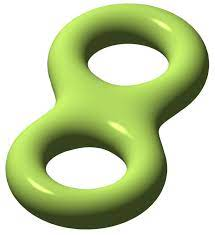
\includegraphics[scale=0.25]{genus-two}
\caption{The two holed torus (surface of genus of 2)}
\label{fig:genus-two}
\end{center}
\end{figure}

$$
\begin{pmatrix}
\text{Topological } \\
\text{spaces}
\end{pmatrix}
\bigleadsto
\begin{pmatrix}
\text{Quantum\,} \\ \text{systems}
\end{pmatrix}.
$$

All of the interesting quantum systems are in two dimensional spaces. This can be seen as follows. TQC is performed by braiding quasiparticles through spacetime. When space is two dimensional, spacetime is three dimensional. When space is three dimensional, spacetime is four dimensional. It is a theorem that there are no knots in four dimensions: The extra dimension gives the knot room to move around and untangle. Thus, to have nontrivial knots, space must be two dimensional. A two dimensional space is called a \textit{surface}. The surfaces we are interested in are those two dimensional spaces which can be embedded into three dimensional space, i.e., those surfaces which can be realized physically in our three dimensional world. Note that there are some weird surfaces which can not be embedded into three dimensional space, such as the Klein bottle (shown in Figure  \ref{fig:klein-bottle}). While the `true' surface does not intersect itself, any way of placing it in three dimensions will self intersect. One needs an extra dimension to avoid this intersection.

\begin{figure}
\begin{center}
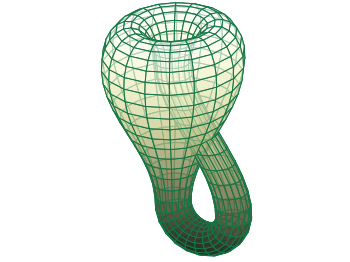
\includegraphics[scale=0.25]{klein-bottle}
\caption{A Klein bottle, attempting to be embedded in 3d space}
\label{fig:klein-bottle}
\end{center}
\end{figure}

This condition on embeddability into three dimensional space makes our study of surfaces much simpler. Namely we have the following well-known theorem from topology:

\begin{theorem} Consider a surface that

\begin{enumerate}
\item Is finite in area (for example, an infinitely stretched flat plane would not count)
\item Has no boundary (for example, a unit disk would not count, since its boundary is the circle)
\item  Can be embedded into three dimensional space.
\end{enumerate}

Then, this surface must be a collection of $g$-holed torii, for some integers $g\geq 0$.
\end{theorem}

Thus, going forward the word `surface' will simply refer to a collection of $g$-holed torii. A connected surface is one which can not be decomposed as the union of two other smaller surfaces. Every connected surface will be the $g$-holed torus for some $g\geq0$, and more general surfaces can all be uniquely written as a union of connected surfaces. A two dimensional topological quantum phase of matter is thus an assignment

$$
\begin{pmatrix}
\text{Surfaces} \\
\text{in space}
\end{pmatrix}
\bigleadsto
\begin{pmatrix}
\text{Quantum\,} \\ \text{systems}
\end{pmatrix}.
$$

Mathematically, a quantum system is a complex vector space. Hence, a topological quantum phase of matter is an assignment

$$S \,\mathlarger{\leadsto}\,V(S),$$

where $S$ is a surface and $V(S)$ is a finite dimensional vector space over the complex numbers. This mathematical formalism is known as Topological Quantum Field Theory. Namely, the assignment $S \,\mathlarger{\leadsto}\,V(S)$ \textit{is} a Topological Quantum Field Theory. To ease terminology, we will from now on use the acronym TQFT.

Not every assignment of surfaces to vector spaces will be a TQFT. Namely, many will be `un physical', meaning that they never could have come from topological phases of matter. For example, the axioms of quantum mechanics say that putting two quantum systems together should correspond to the tensor product of those systems. Formally, we should have

$$V\left(S_0\sqcup S_1\right)=V(S_0)\otimes V(S_1).$$

Here, $\sqcup$ denotes the disjoint union. The disjoint union is the same as a union, but it specifies that the union should be taken in a way such that $S_0$ and $S_1$ do not intersect (i.e. that they are disjoint). The disjoint union can be intuitively read as simply putting two spaces next to each other.

Additionally, by the axioms of quantum mechanics, transformations of a surface through spacetime should correspond to linear maps on quantum systems. We think mathematically about what a trajectory through spacetime looks like. In the one dimensional case, suppose we have two particles $a$ and $b$. A trajectory through spacetime from $a$ to $b$ is a path $e$ connecting $a$ and $b$. Thinking deeply, one observes that the condition of ``connecting" $a$ and $b$ can be mathematically stated as $\partial e= a \sqcup b$, where $\partial e$ denotes the boundary of $e$. This is shown in Figure \ref{fig:bordism}.

\begin{figure}
\begin{center}
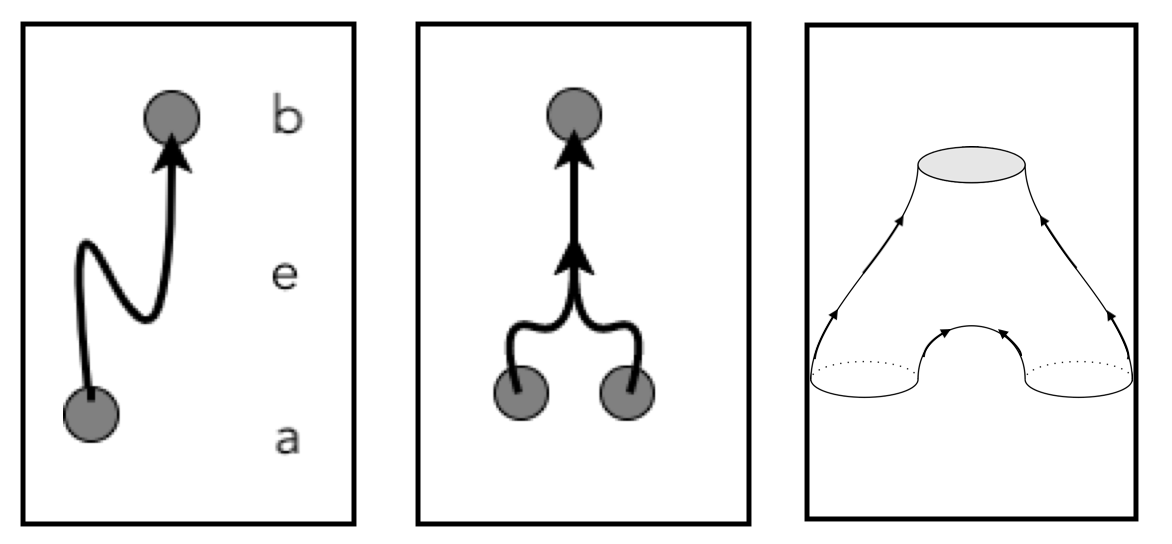
\includegraphics[scale=0.40]{cobordism}
\caption{First box - A path in spacetime from $a$ to $b$ by $e$, i.e., a path $e$ with $\partial e= a \sqcup b$. Second box - The fusion of two particles in spacetime. Third box - the fusion of two circles in spacetime, known informally as a ``Pair of Pants".}
\label{fig:bordism}
\end{center}
\end{figure}

We observe however an ambiguity: Time has direction, but our edge a-priori does not. Hence, it is impossible to distinguish a path from $a$ to $b$ and a path from $b$ to $a$. For this reason we have to introduce the concept of \textit{orientation}. An oriented path is a path with a choice of direction. This can be visualized by putting a consistent set of arrows on the path. The points at the back end of the arrow correspond to the particles at the start of the process, and the points at the front end of the arrow correspond to the particles at the end of the process. Note that the paths can join and split, as seen in the second box of Figure  \ref{fig:bordism}. This corresponds to the fusion and annihilation of particles.

Working one dimension higher, we can imagine the trajectory of circles of particles - loops - through spacetime. The merging of two circles will look exactly like it did before, except that now instead of tracing a path through spacetime it will trace a surface with boundary. The boundary components correspond exactly to the particles at the start and end of the process, as seen in the third box of Figure \ref{fig:bordism}.

We now try to generalize this picture to the case of surfaces. Remember, our goal is to mathematically describe a trajectory of surfaces through spacetime, which will be key to our theory since these will correspond to linear transformations on quantum systems. The key insight is as follows. Given two sets of $A$ and $B$ (still representing particles), we saw a trajectory through spacetime was a path $E$ such that $\partial E=A\sqcup B$. Given two collections of circles $A$ and $B$, we saw a trajectory through spacetime was a surface $E$ such that $\partial E=A\sqcup B$. Given two surfaces $S_0$ and $S_1$ (with no boundary, as usual), a trajectory through spacetime should be a three dimensional object $X$ whose boundary is $\partial X= S_0\sqcup S_1$.

Defining what we mean exactly by three dimensional object is very technical. Namely, these objects should be $3$-manifolds, in the same way that a surface is a $2$-manifold, a path is a $1$-manifold, and a set of points is a $0$-manifold. An introduction to the theory of manifolds can be found in Spivak's textbook \cite{spivak2018calculus}. We leave the notion vague. One can think of 3-manifolds as being filled in surfaces. For instance, the torus is a surface ($2$-manifold), but the filled in solid torus is a $3$-manifold. Let $X$ be the solid torus with a smaller solid torus removed from inside it. Then the boundary $\partial X$ will be equal to the disjoint union of the outside torus and the smaller inside torus. We can see that $X$ forms a trajectory through spacetime, as the bigger torus contracts onto the smaller one. There is still one ambiguity. How do we know that $X$ is a contraction big to small? Instead, it could have been an expansion small to big. To fix this issue we will again have to speak of oriented $3$-manifolds. Oriented manifolds are (loosely) manifolds with a coherent system of arrows giving direction at every point. For example, a series of arrows in $X$ all pointing from the big outside torus toward the smaller inside torus is an orientation.

We introduce a piece of notation. When $\partial X = S_0 \sqcup S_1$ is the disjoint union of two surfaces, one of those surfaces (say, $S_0$) will always be the stuff going in, and one of those surfaces (say, $S_1$) will always be the stuff going out. We call this a \textit{bordism}\footnote{Sometimes called a cobordism; the difference is immaterial.} from $S_0$ to $S_1$. Namely, a bordism from a surface $S_0$ to a surface $S_1$ is an oriented $3$-manifold $X$ such that $\partial X = S_0\sqcup S_1$, where all of the arrows in the orientation of $X$ are pointing away from $S_0$ and towards $S_1$ . With this out of the way, we can formally define a TQFT:

\begin{definition}[$(2+1)$-TQFT] A $(2+1)$ Topological Quantum Field Theory (TQFT) is the following data.
\begin{enumerate}
\item A choice of finite dimensional complex vector space $V(S)$ for every surface $S$.
\item A choice of linear transformation $Z(X): S_0\xrightarrow{} S_1$ for every bordism $X$ from $S_0$ to $S_1$.
\end{enumerate}
Additionally, a $(2+1)$-TQFT is required to satisfy the following properties:
\begin{enumerate}

\item (Union = tensor product). $V(S_0\sqcup S_1)=V(S_0)\otimes V(S_1)$. Here, $S_0$ and $S_1$ are any two surfaces.

\item (Do nothing = identity) $Z(S\times [0,1])=\text{id}_{V(S)}$. Here, $S\times [0,1]$ is the Cartesian product of $S$ with the interval, treated as a bordism from $S$ to itself. Concretely $\partial (S\times [0,1])=S\times\{0\}\sqcup S\times\{1\}$, and we identify $S\times \{0\}$ and $S\times\{1\}$ both with $S$.

\item (Composing bordisms = composing maps). $Z(X_1\cup X_0)=Z(X_1)\circ Z(X_0)$. Here, $X_0$ is a bordism from two surfaces $S_0$ and $S_1$ and $X_1$ is a bordism from surfaces $S_1$ to $S_2$. One easily verifies that their union $X_1\cup X_0$ is a bordism between $S_0$ and $S_2$, whose induced map we can compare with the composition of the induced maps of $X_0$ and $X_1$.

\item (Swap spaces = swap tensor factors) $Z(X)(v_0\otimes v_1)=v_1\otimes v_0$ for all $v_0\in V(S_0)$, $v_1\in V(S_1)$. Here, $X$ is the bordism from $S_0\sqcup S_1$ to $S_1\sqcup S_0$ defined by taking $S_0,S_1$ and moving them around each other. 
\end{enumerate}

\raggedleft\qedsymbol{}

\end{definition}

We offer a few remarks. The term ``$(2+1)$" refers to the fact that there are two space dimensions, plus one time dimension. More generally, an  $(n+1)$-TQFT is an assignment of $n$-manifolds to vector spaces, and of $(n+1)$-manifolds to linear transformations. We also remark on the structure of the definition. We first defined a few assignments of objects of one type to objects of another type, and then we defined a laundry list of properties that those assignments should satisfy. This is extremely standard practice in higher mathematics. The abstraction of this practice is known as Category Theory. The assignments of one type of object to another type of object are known as functors, and the properties to satisfy are known as axioms. The category theory definition of a TQFT is ``a symmetric monoidal functor from the category of bordisms to the category of vector spaces"\footnote{symmetric=axiom 4, monoidal=axiom 1, functor=axiom 3, bordsism category=axiom 2}. For those unfamiliar with category theory, a short introduction is found in Appendix \ref{Categories}. While we will not be using any categories in this section, a familiarity of the subject is required for the following section on Modular Tensor Categories.

Often, TQFTs will be defined in terms of celluations. A celluation is a way of splitting up a space into vertices, edges, and faces. The utility of celluations is that they turn continuous objects into discrete ones, which allows for simple computations - this was the entire point of modeling the torus as an $n$ by $n$ grid in Section \ref{The Toric Code}. The difficult part is often showing that the object you defined is independent of the choice of celluation. For the toric code, this was Exercise \ref{The Toric Code}.3. In general, one resorts to the following theorem:

\begin{theorem}[Pachner, \cite{pachner1991pl}, \cite{lickorish1999simplicial}]\label{Pachner} Let $(X,\Delta_X)$ and $(X,\Delta'_X)$ be two manifolds with triangulations (i.e. celluations in which every face has three edges). There exists a finite sequence of so-called Pachner moves relating $\Delta_X$ to $\Delta'_X$. In two dimensions (i.e. when $X$ is a surface) and three dimensions, the full list of Pachner moves is given in Figure \ref{fig:all-moves}. The naming convention is that the ``$a$-$b$" move is the move that takes $a$ cells to $b$ cells.
\end{theorem}

\begin{figure}
\begin{center}
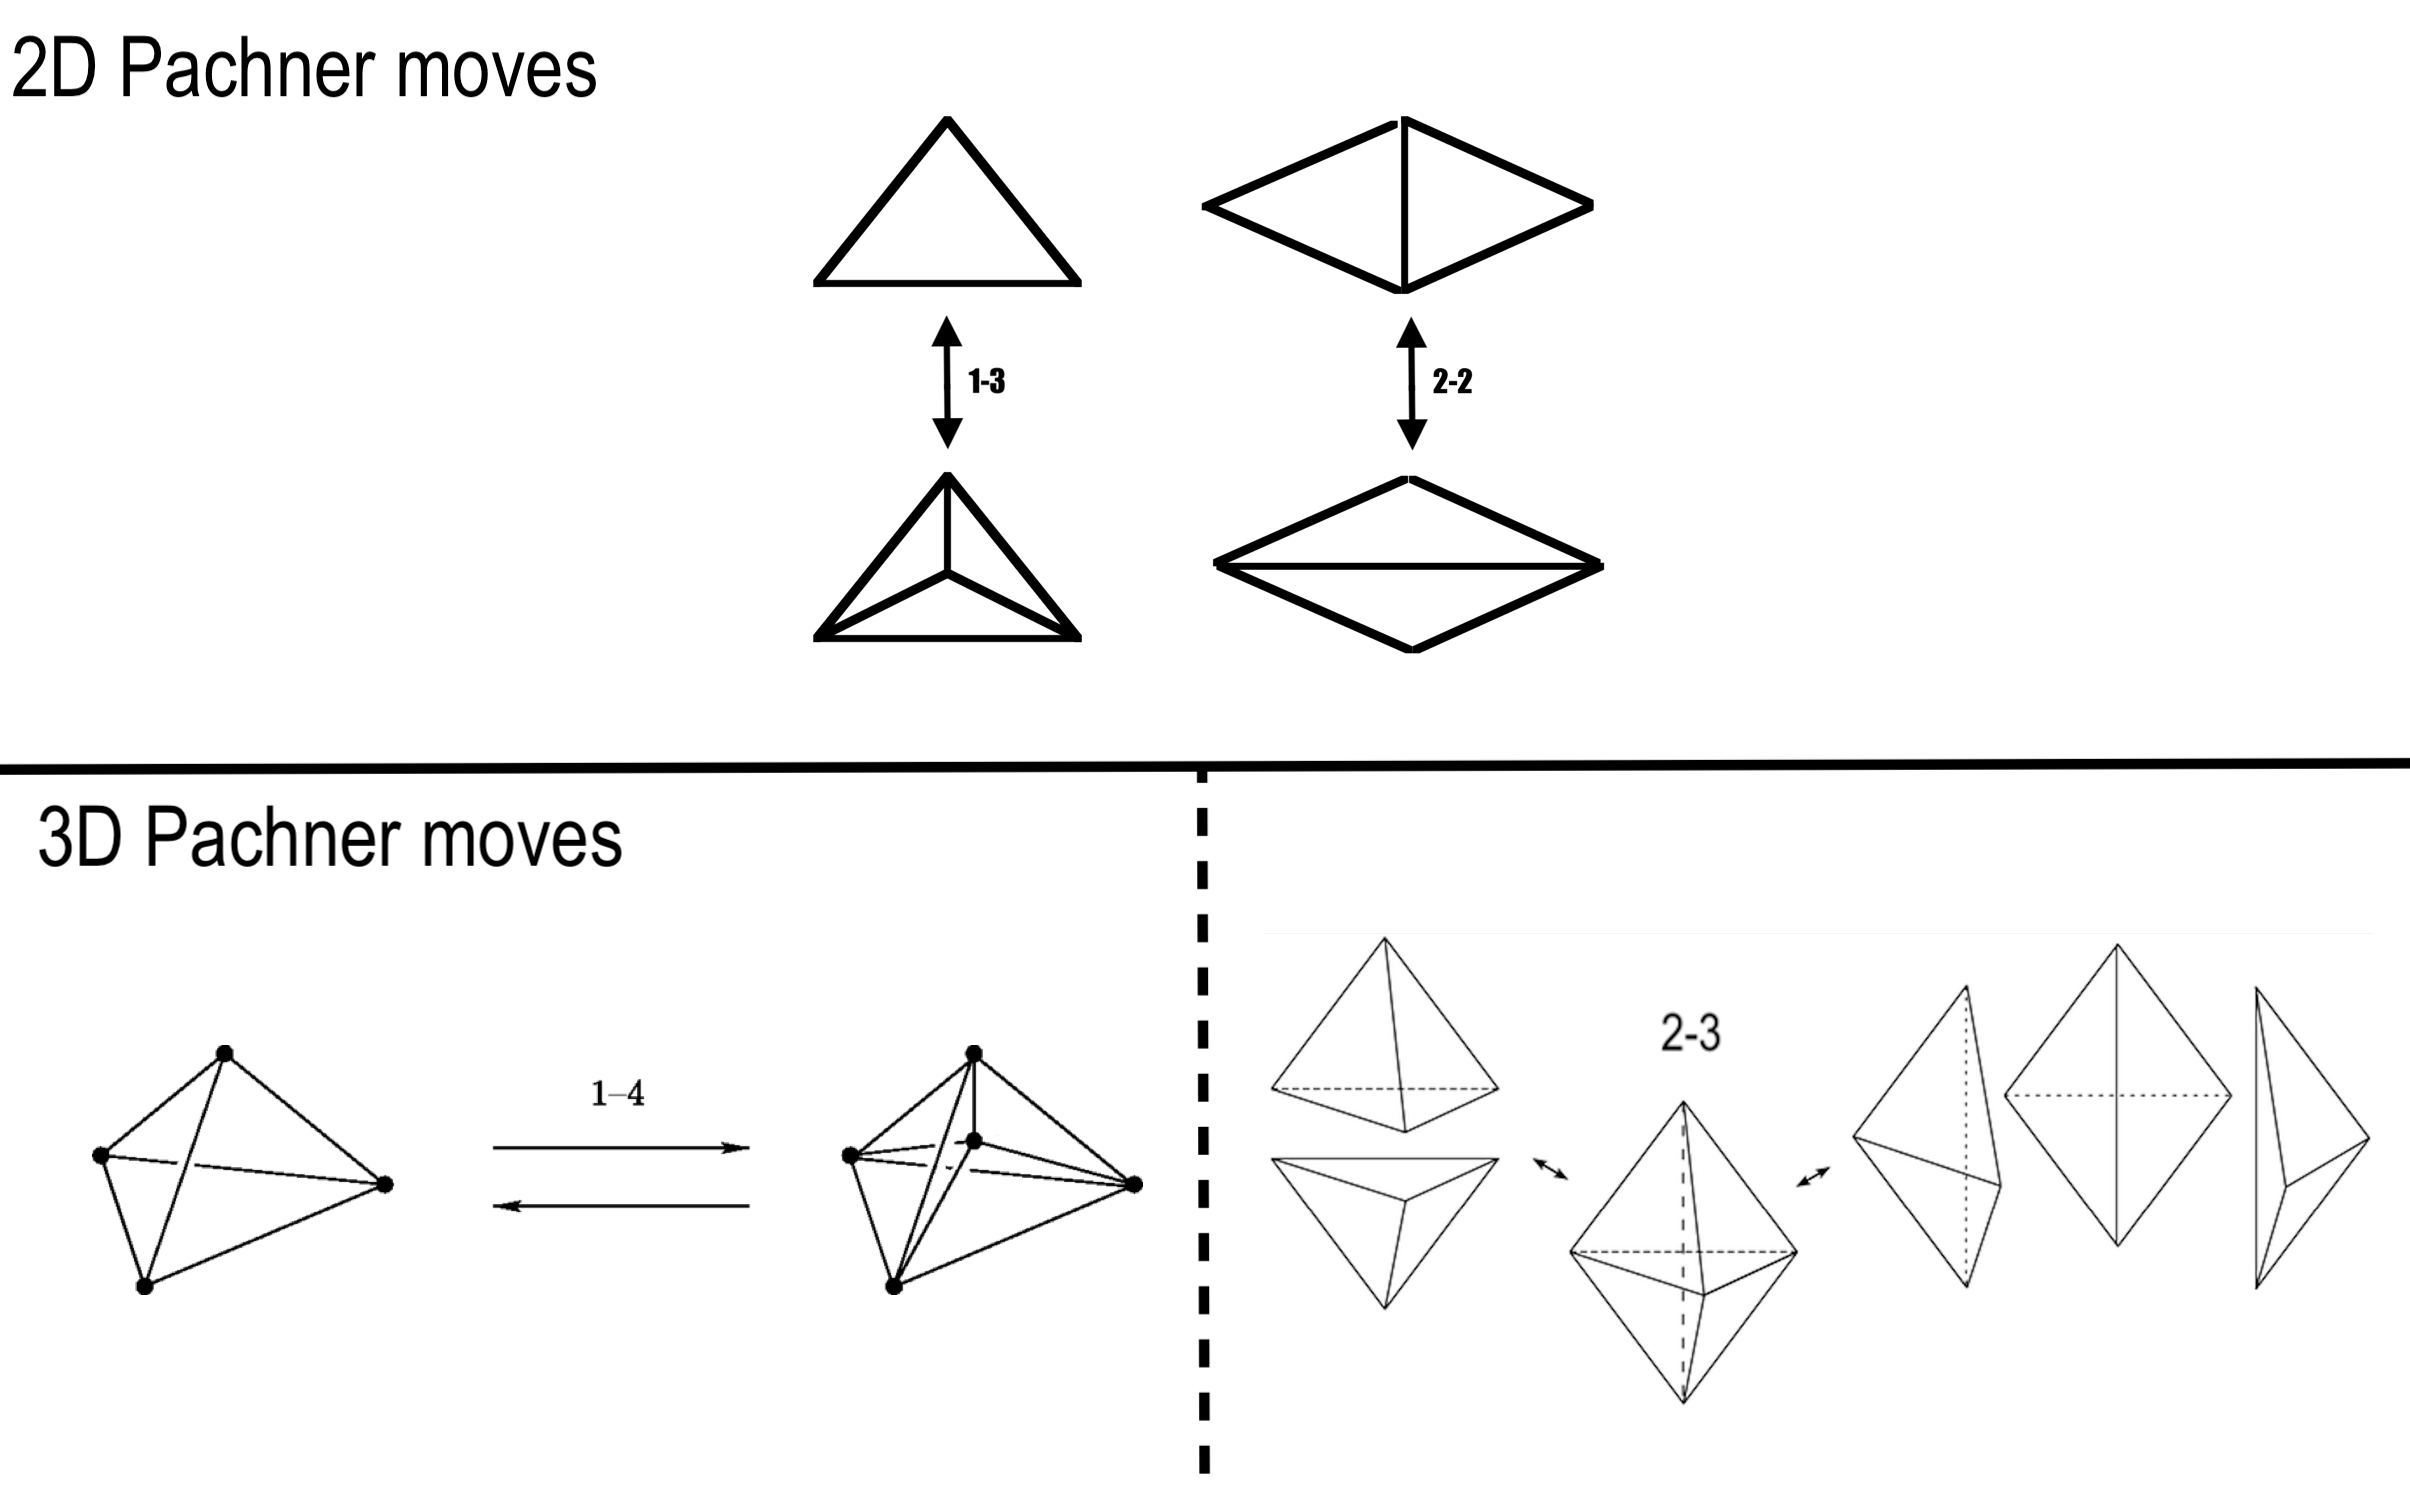
\includegraphics[scale=0.2]{all-moves}
\caption{The Pachner moves.}
\label{fig:all-moves}
\end{center}
\end{figure}


This massively facilitates the verification of whether or not a definition is independent of celluation. Namely, first you show that the definition is invariant under adding/removing edges (allowing you to turn the celluation into a triangulation), and then you check that the definition is invariant under applying the Pachner moves. Typically, this verification is entirely elementary and does not require any great show of cleverness. As such, our standard practice for  Subsection \ref{DW TQFT} will be to state theorems, reduce the problem to the verification of invariance under Pachner moves, and assign the rest as an exercise to the reader.

\subsection{The $\ZZ_2$ Dijkgraaf-Witten TQFT}
\label{DW TQFT}

We now define the Topological Quantum Field Theory (TQFT) associated with the toric code, and describe how TQC can be performed in this framework. We could also call it the ``$\ZZ_2$ spin liquid TQFT", since it is the mathematical realization of the $\ZZ_2$ spin liquid topological quantum phase of matter. The original reference for this subject is \cite{dijkgraaf1990topological}, but our presentation follows more closely \cite{qiu2021representations}.

As with the definition of the toric codes in Section \ref{The Toric Code}, the definition of the $\ZZ_2$ Dijkgraaf-Witten TQFT is in the language of $\ZZ_2$ homology. Seeing as our definition of homology requires a celluation we first define $\tilde{V}(S,\Delta)$, where $S$ is a surface and $\Delta_S$ is a celluation of $S$. That is, $\Delta_S$ is a representation of $S$ as a collection of vertices, edges, and faces, with some edges and vertices identified. For example, $S=T$ could be the torus, and $\Delta$ could be the $n$ by $n$ lattice with opposite edges identified. For every surface $S$ and celluation $\Delta_S$, we define

$$\tilde{V}(S,\Delta_S)=\CC\left[C^{1}(\Delta_S;\ZZ_2)\right].$$

Here $C^1(\Delta_S;\ZZ_2)$ denotes the group $\ZZ_2$ cocycles on the celluation $\Delta_S$, and $\CC[-]$ is notation for ``complex vector space generated by", i.e., $\tilde{V}(S)$ is the unique complex vector space having $C^1(\Delta_S;\ZZ_2)$ as a basis. A $\ZZ_2$ cocycle is an assignment of $0$s and $1$s to every edge, such that every face touches an even number of $1$-labeled edges.

Notice that a $\ZZ_2$ cocycle is the same thing as a $\ZZ_2$ cycle in the dual celluation, as discussed in the proof of Proposition \ref{Xparticle}. That is, every $\ZZ_2$ cocycle on $S$ specifies a cycle on $S$, by drawing lines between the centers of two faces whenever the edge connecting them is labeled by a $1$. This process of identifying cocycles on $\Delta_S$ and cycle in the dual celluation is known as Poincaré Duality. It is important to note that in higher dimensions the process breaks down, because generically loops will fail to intersect in three dimensions (they can just be shifted past each other). Thus, when discussing 3-manifold bordisms there is a real distinction between cycles and cocycles.

The reason we call this $\tilde{V}$ instead of $V$ is that it depends on the choice of celluation $\Delta_S$, and we want $V(S)$ to only depend on $S$. The invariant subspace $V(S)$ is defined like so:

$$V(S)=\CC[H^1(S;\ZZ_2)],$$

where $H^1(S;\ZZ_2)$ is the cohomology of $S$. Cohomology is defined by

$$H^1(S;\ZZ_2)=C^1(S;\ZZ_2)/Z^1(S;\ZZ_2),$$

where $Z^1(S;\ZZ_2)$ is the subgroup of $C^1(S;\ZZ_2)$ generated by the cocycles consisting of $1$s at every edge touching a vertex. Assigning $1$s and $0$s this way really does give a cocycle: Every face has either $0$ or $2$ edges in its boundary that touch a given vertex, and both $0$ and $2$ are even numbers. It is a standard fact that the cohomology of a space does not depend on the choice of celluation.

To view $V(S)$ and a subspace of $\tilde{V}(S,\Delta_S)$, we define a linear injection

\begin{align*}
V(S)&\hookrightarrow \tilde{V}(S,\Delta_S).\\
\left|\alpha\right>&\mapsto \frac{1}{\sqrt{|Z^1(S;\ZZ_2)|}}\sum_{\gamma\sim \alpha}\left|\gamma\right>
\end{align*}

Here, $\alpha$ is a cohomology class (an element of $H^1(S;\ZZ_2)$), $\left|\alpha\right>$ is the corresponding vector in $V(S)$, $|Z^1(S;\ZZ_2)|$ denotes the number of elements in $Z^1(S;\ZZ_2)$, and $\sim$ denotes the equivalence relation of being cohomologous. That is, two cocycles are cohomologous if they give the same element in $H^1(S;\ZZ_2)$. This map can be summarized by saying that a cohomology class sends to the equal superposition of all of its representatives. The normalizing factor $|Z^1(S;\ZZ_2)|^{-1/2}$ is introduced to make sure that the norm is preserved.

We now define the action of bordisms. Let $(S_0,\Delta_{S_0})$ and $(S_1,\Delta_{S_1})$ be two surfaces with celluations. Let $X$ be a bordism from $S_0$ to $S_1$. Let $\Delta_X$ be a celluation on $X$ compatible with the celluations on $S_0$ and $S_1$. By compatible we mean that if we restrict $\Delta_X$ to $\partial X$ then we will recover the celluations $\Delta_{S_0}$ and $\Delta_{S_1}$. This restriction process can be described visually as dropping all verticies, edges, and faces, from $\Delta_X$ that aren't part of $\partial X=S_0\sqcup S_1$. We call a pair of cocycles $(\omega_{S_0},\omega_{S_1})$ extendable if there is a cocycle in $\omega_X\in C^1(X,\Delta_X)$ which gives $\omega_{S_0}$ when restricted to $S_0$ and $\omega_{S_1}$ when restricted to $S_1$. Let $N_X$ be the number of cocycles in $C^1(S_1;\ZZ_2)$ with which the $0$ cocycle on $S_0$ can be extended. We define

$$\tilde{Z}(X,\Delta_X)=\frac{1}{N_X}\begin{pmatrix}
$1$\text{ if }(\omega_{S_0},\omega_{S_1})\text{ extendable}\\
$0$\text{ otherwise }
\end{pmatrix}_{\substack{\omega_{S_0}\in C^1(S_0;\ZZ_2) \\ \omega_{S_1}\in C^1(S_1;\ZZ_2)}}.$$

We now elaborate on the meaning of this expression. Linear algebra tells us that to specify a linear transformation between two spaces, all we need to do is specify the entries of a matrix. The entries of a matrix are labeled by basis vectors. Namely, the matrix entries of a map from $\CC[C^1(S_0;\ZZ_2)]$ to $\CC[C^1(S_1;\ZZ_2)]$ are labeled by ordered pairs of basis vectors $(\left|\omega_{S_0}\right>,\left|\omega_{S_1}\right>)$, where $\omega_{S_0}\in C^1(S_0;\ZZ_2)$ and $\omega_{S_1}\in C^1(S_1;\ZZ_2)$. The $(\left|\omega_{S_0}\right>,\left|\omega_{S_1}\right>)$ entry in $\tilde{Z}(X;\Delta_X)$ is equal to $1$ if $(\omega_{S_0},\omega_{S_1})$ is extendable, and $0$ otherwise.

The intuition for $\tilde{Z}(X,\Delta_X)$ comes from the path integral formulation of quantum mechanics. When not being observed, a system will transform along an equal superposition of all possible trajectories. There is a spacetime trajectory sending a state (cocycle) $\left|\omega_{S_0}\right>$ to a state (cocycle) $\left|\omega_{S_1}\right>$ exactly when $(\omega_{S_0},\omega_{S_1})$ can be extended. The map $\tilde{Z}(X,\Delta_X)$ can be described as the transformation that takes a state to the equal superposition of all possible states it could go to.

Our goal is to show that $\tilde{Z}(X,\Delta_{X})$ restricts to a map $V(S_0)\xrightarrow{}V(S_1)$, and that this restriction is independent of our choice of $\Delta_{S_0}, \Delta_{S_1}$ and $\Delta_{X}$. Once this has been done we can define $Z(X)$ to be this common restriction. All that will be left to do then is to show that our assignments $V(S)$ and $Z(X)$ satisfy the axioms of a $(2+1)$-TQFT. We work on this overarching plan over the course of a few propositions.

\begin{proposition}\label{Celluation independent}
Let $(S_0,\Delta_{S_0})$ and $\left(S_1,\Delta_{S_1}\right)$ be surfaces with celluations, $X$ a bordism from $S_0$ to $S_1$, and $\Delta_X$ a celluation of $X$ compatible with the celluations on $S_0$ and $S_1$. Then, the map $\tilde{Z}(X,\Delta_X): \tilde{V}(S_0,\Delta_{S_0})\xrightarrow{}\tilde{V}(S_1,\Delta_{S_1})$ is independent of the choice of celluation $\Delta_X$. Hence, we can properly omit $\Delta_X$ from our notation, and speak of a well defined map $\tilde{Z}(X)$.
\end{proposition}
\begin{proof} We need to show that if $\Delta_X$ and $\Delta'_X$ are two different choices of celluations on $X$ compatible with $\Delta_{S_0}$ and $\Delta_{S_1}$, then then $\tilde{Z}(X,\Delta_X)=\tilde{Z}(X,\Delta'_X)$. That is, $(\omega_{S_0},\omega_{S_1})$ are extendable in $\Delta_X$ if and if they are extendable in $\Delta_X'$. By Theorem \ref{Pachner}, all we have to do is show that the property of $(\omega_{S_0},\omega_{S_1})$ being extendable is invariant first under the operation of adding/removing edges (to turn the celluation into a triangulation), and secondly invaraint under the process of applying Pachner moves. Drawing out the diagrams, these are straightforward computations. We leave the verification of the proof as an exercise to the reader (Exercise \ref{TQFTs}.1).
\end{proof}

\begin{lemma}\label{independence} Let $(S_0,\Delta_{S_0})$, $(S_1,\Delta_{S_1})$, $(S_1,\Delta_{S_2})$ be surfaces with celluations, let $X_0$ be a bordism from $S_0$ to $S_1$, and let $X_1$ be a bordism from $S_1$ to $S_2$.

\begin{enumerate}[(i)]
\item $|\left\{\omega_{S_1}\in C^1(\Delta_{S_1};\ZZ_2) \st (\omega_{S_0},\omega_{S_1}) \text{ extendable}\right\}|$ is independent of choice of $\omega_{S_0}$
\item $|\left\{\omega_{S_1}\in C^1(\Delta_{S_1};\ZZ_2)\st (\omega_{S_0},\omega_{S_1})\,\, \& \,\,(\omega_{S_1},\omega_{S_2})\text{ extendable}\right\}|$ is independent of choice of $\omega_{S_0}$, $\omega_{S_2}$, so long as $(\omega_{S_0},\omega_{S_2})$ is extendable
\end{enumerate}
\end{lemma}
\begin{proof} We prove $(i)$, and leave $(ii)$ as an exercise (Exercise $\thesection.2$) since the proof is identical. Let $\omega_{S_1}$ and $\omega_{S_1}$ be such that $(\omega_{S_0},\omega_{S_1})$ and $(\omega_{S_0},\omega'_{S_1})$ are extendable. Then, adding extensions of these pairs together edgewise we get that $(\omega_{S_0}+\omega_{S_0},\omega_{S_1}+\omega'_{S_1})$ is extendable. Since $\omega_{S_0}+\omega_{S_0}=0$, we find that there is a $1$-to-$1$ bijection between $\omega_{S_1}$ such that $(0,\omega_{S_1})$ is extendable and $\omega_{S_1}$ such that $(\omega_{S_0},\omega_{S_1})$ is extendable, sending $\omega_{S_1}$ to $\omega_{S_0}+\omega_{S_1}$ Thus, these sets have the same cardinality, and we conclude $(i)$.
\end{proof}

\begin{proposition}\label{composition} Letting $X_0,X_1$ be as in Lemma \ref{independence}, the composition law

$$Z(X_1\cup X_0)=Z(X_1)\circ Z(X_0)$$

holds.
\end{proposition}
\begin{proof} Expanding by matrix multiplication, we find by the definition of $Z(X)$ that the coefficient of $(\omega_{S_0},\omega_{S_2})$ in $Z(X_1)\circ Z(X_0)$ is

$$\frac{1}{N_{X_0}N_{X_1}}\sum_{\omega_{S_1}}
\begin{pmatrix}
$1$\text{ if }(\omega_{S_0},\omega_{S_1})\text{ extendable}\\
$0$\text{ otherwise }
\end{pmatrix}
\begin{pmatrix}
$1$\text{ if }(\omega_{S_1},\omega_{S_2})\text{ extendable}\\
$0$\text{ otherwise }
\end{pmatrix}.$$

The coefficient of $(\omega_{S_0},\omega_{S_2})$ in $Z(X_1\cup X_0)$ is $N^{-1}_{X_1\cup X_0}$ if $(\omega_{S_0},\omega_{S_2})$ extendable, and $0$ otherwise. Multiplying through, we find the equality we are trying to prove is

$$N_{X_0\cup X_1} |\left\{\omega_{S_1}\st (\omega_{S_0},\omega_{S_1})\,\, \& \,\,(\omega_{S_1},\omega_{S_2})\text{ extendable}\right\}|=N_{X_0} N_{X_1}.$$

Fix $\omega_{S_0}$. We claim that both sides of the above expression are equal to the number of pairs $(\omega_{S_1},\omega_{S_2})$ such that $(\omega_{S_0},\omega_{S_1})$ and $(\omega_{S_1},\omega_{S_2})$ are simultaneously extendable. The left hand side computes this value by first counting the number of ways of choosing $\omega_{S_2}$ (i.e. $N_{X_0\cup X_1}$), and the by counting the number of ways of filling in $\omega_{S_1}$. The right hand side computes this value by first counting the number of ways of choosing $\omega_{S_1}$ (i.e. $N_{X_0}$) and then counting the number of ways of choosing $\omega_{S_2}$ (i.e. $N_{X_1}$). Note the implicit use of Lemma \ref{independence}, saying that all of these values are equal. This completes the proof.

\end{proof}

The next proposition has a strong physical meaning, and can be seen as motivation for the fact that $V(S)$ is a ground state space. Namely, let $(S,\Delta_S)$ be a surface with celluation and let $S\times [0,1]$ be the product of $S$ with the real interval of numbers between $0$ and $1$. That is, elements of $S\times [0,1]$ are pairs $(s,t)$ where $s\in S$ and $t\in [0,1]$. This is a $3$-manifold, and gives a bordism from $S$ to itself. Namely, $\partial (S\times [0,1])$ is built of the two components $S\times \{0\}$ and $S\times \{1\}$. The orientation on $S\times [0,1]$ is induced by the orienation on $[0,1]$. This can viewed as the identity bordism: $S$ is doing nothing as time increases from $0$ to $1$. The boundary components correspond to the placement of $S$ at time $0$ and $S$ at time $1$. When time passes on a system, we expect it to ambiently decrease in energy. Thus,  physically $Z(S\times [0,1])$ should act by the identity on ground states, and send higher energy states down to the ground state. This is exactly the statement that $Z(S\times [0,1])$ should be a projection from the full state space to the ground state space. The following proposition in this lens thus says that $V(S)$ are exactly the ground space:

\begin{proposition}\label{Z formula} Let $(S,\Delta_S)$ be a surface with celluation. Viewing $S\times [0,1]$ as a bordism from $S$ to itself, we have that $\tilde{Z}(S\times [0,1])$ is a projection from $\tilde{V}(S,\Delta_S)$ to $V(S)$. Namely, the image of $\tilde{Z}(S\times [0,1])$ is $V(S)$, and $\tilde{Z}(S\times [0,1])$ acts by the identity on $V(S)$. Explicitly, $\tilde{Z}(S\times [0,1])$ is given by the map

$$\left| \omega\right>\mapsto \frac{1}{|Z^1(\Delta_{S};\ZZ_2)|}\sum_{\gamma \sim \omega}\left|\gamma\right>.$$

\end{proposition}
\begin{proof} Let $\omega_{S}$, $\omega'_{S}$ be two cocycles on $\Delta_{S}$. We show that $(\omega_{S},\omega_{S}')$ is extendable if and only if $\omega_{S}$ and $\omega_{S}'$ are cohomologous. Consider the celluation $\Delta_{S\times [0,1]}$ obtained by adding an edge connecting each vertex in $S\times\{0\}$ to the corresponding vertex in $S\times \{1\}$.

\begin{figure}
\begin{center}
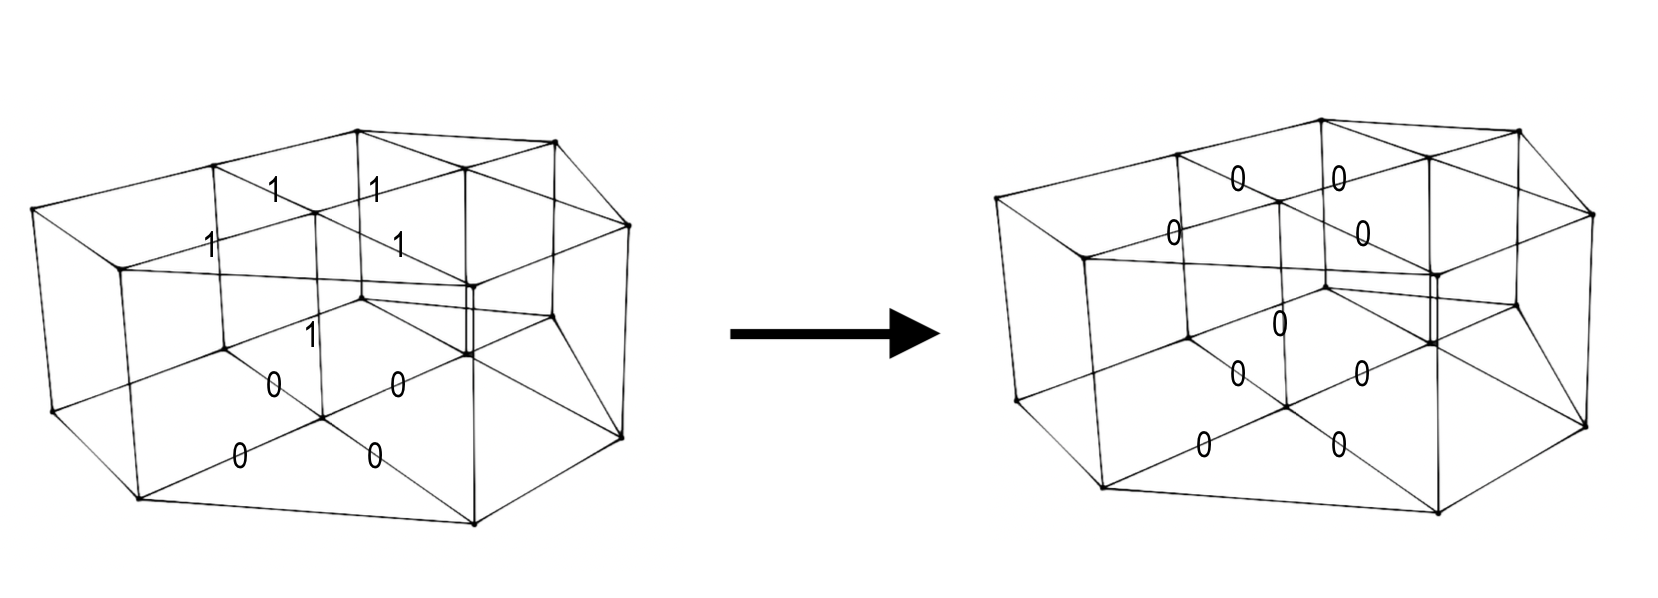
\includegraphics[scale=0.3]{cohomologous}
\caption{Removing the 1s from the central edges in $S\times [0,1]$}
\label{fig:cohomologous}
\end{center}
\end{figure}

We proceed by induction on the number of central edges in $S\times [0,1]$ (i.e. edges of $S\times [0,1]$ not in the boundary) which are assigned the value $1$ in the extension $\omega_X$ of $(\omega_{S},\omega_{S}')$. If there are no such edges, then clearly we must have $\omega_{S}=\omega_{S}'$, and so our proof is complete. Suppose there is a nonzero amount of such edges. Choose a central edge $e$ assigned $1$ in $\omega_X$. Let $\omega'_X$ the the cocycle obtained by flipping $e$ to as $0$, as well as flipping all of the edges touching $e$ in $S\times\{1\}$. $\omega'_X$ satisfies the cocycle condition since faces in the center touching $e$ will also touch exatly one of the edges flipped in $S\times \{1\}$, and hence the sum $1$s around the edges of those faces will change an even amount. By our inductive hypothesis, we conclude that $\omega_{S}'$ and $\omega_{S}$ are cohomologous. This process is demonstrated in Figure \ref{fig:cohomologous}.

The number of ways $N_{S\times [0,1]}$ of extending the $0$ cocycle is thus equal to the number of cocycles cohomologous to $0$, which is by definition $|Z^1(\Delta_S;\ZZ_2)|$. Thus, the stated formula is correct. It is straightforward to see that the rest of the proposition follows immediately from this formula.
\end{proof}

This allows us to prove the full independence of our theory from choice of celluation:

\begin{proposition}\label{S0S1 independence} Let $(S_0,\Delta_{S_0})$ and $\left(S_1,\Delta_{S_1}\right)$ be surfaces with celluations, and let $X$ be a bordism from $S_0$ to $S_1$. The image of $\tilde{Z}(X)$ is contained in $V(S_1)$. In particular, $\tilde{Z}$ restricts to a map $V(S_0)\xrightarrow{}V(S_1)$. This map is independent of our choice of $\Delta_{S_0}$ and $\Delta_{S_1}$. We define $Z(X): V(S_0)\xrightarrow{}V(S_1)$ to be this common restriction.
\end{proposition}
\begin{proof} To begin, we observe that if $(\omega_{S_0},\omega_{S_1})$ is extendable, then so is $(\omega'_{S_0},\omega_{S_1})$ for any $\omega'_{S_0}$ homologous to $\omega_{S_0}$. This follows by precomposing $X$ with $S_0\times [0,1]$, which does not change $X$, first extending $(\omega'_{S_0},\omega_{S_0})$ by Proposition \ref{Z formula}, and then extending $(\omega_{S_0},\omega_{S_1})$.

Thus, the equal superposition $\left|\omega_{S_0}\right>$ of every cocycle homologous to $\omega_{S_0}$ will map  under $\tilde{Z}(X,\Delta_X)$ to a sum of equal superpositions of cohomologous classes in $H^1(S_1;\ZZ_2)$, i.e., an element of $V(S_1)$. What is left to check is whether or not a cohomology class in $S_0$ can be lifted to a cohomology class in $S_1$ is independent of the choices of celluations.

To prove this, we consider the identity bordism $S\times [0,1]$ with $S\times \{0\}$ given a celluation $\Delta_{S}$ and $S\times \{1\}$ given a celluation $\Delta'_S$. We show that a cocycle in $C^1(\Delta_{S};\ZZ_2)$ can be lifted to a class in $C^1(\Delta'_{S};\ZZ_2)$ if and only if they are homologous. Applying this with $S=S_0$ and precomposing with $S_0\times [0,1]$ gives the desired independence of choice of celluation on $S_0$, and applying this with $S=S_1$ and postcomposing with $S_1\times [0,1]$ gives the desired independence of choice of celluation on $S_1$.

The above claim again follows from applying induction with respect to the moves in Theorem \ref{Pachner}, and thus is left as an exercise (Exercise $\thesection.3$).
\end{proof}

The main result of our section is as follows:

\begin{theorem} The assignments $S\mapsto V(S)$ and $X\mapsto Z(X)$ give a Topological Quantum Field Theory, called the $\ZZ_2$ Dijkgraaf-Witten TQFT.
\end{theorem}
\begin{proof} We check that our choices of $V(S)$ and $Z(X)$ satisfy the four axioms.

\begin{enumerate}
\item Specifying a cohomology class on $S_0\sqcup S_1$ amounts to specifying a cohomology class on $S_0$, and a cohomology class on $S_1$. In other words, we have a natural equality

$$H^1(S_0\sqcup S_1;\ZZ_2)=H^1(S_0;\ZZ_2)\times H^1(S_1;\ZZ_2).$$

Additionally, for any sets $A$ and $B$ we have $\CC[A\times B]=\CC[A]\otimes \CC[B]$, where we identity $[(a,b)]$ with $[a]\otimes [b]$, $a\in A$, $b\in B$. Thus,

\begin{align*}
V(S_0\sqcup S_1)&=\CC\left[H^1(S_0\sqcup S_1;\ZZ_2)\right]\\
&=\CC\left[H^1(S_0;\ZZ_2)\times H^1(S_1;\ZZ_2)\right]\\
&=\CC\left[H^1(S_1;\ZZ_2)\right]\otimes \CC\left[ H^1(S_1;\ZZ_2)\right]\\
&=V(S_0)\otimes V(S_1).
\end{align*}

\item This follows immediately from Proposition \ref{Z formula}.
\item This follows immediately from Proposition \ref{composition}.
\item The bordism $X$ has the effect of swapping $S_0$ and $S_1$, hence sends $H^1(S_0;\ZZ_2)\times H^1(S_1;\ZZ_2)$ to $H^1(S_1;\ZZ_2)\times H^1(S_0;\ZZ_2)$, sending $(\omega_{S_0},\omega_{S_1})$ to $(\omega_{S_1},\omega_{S_0})$. Tracing through the series of equalities in part 1, we get the desired result.
\end{enumerate}
\end{proof}

Seeing that the $\ZZ_2$ Dijkgraaf-Witten TQFT applied to the torus yields the toric code as defined in Section \ref{The Toric Code} is simple. The only difficulty comes from the fact that as defined, the toric code is generated by homology classes and the $\ZZ_2$ Dijkgraaf-Witten TQFT is generated by cohomology classes. However, as mentioned before, there is a duality between homology classes and cohomology classes which arises from considering the dual celluation, and so this discrepancy is really not an issue. We decided to work with homology in Section \ref{The Toric Code} for pedagogical reasons: homology is more intuitive than cohomology. However, for 3-manifolds there is a discrepancy between homology and cohomology, which is why the $\ZZ_2$ Dijkgraaf-Witten TQFT has to use the less intuitive concept.

In general, there is no Hamiltonian in TQFTs. The lowest energy states are those which will naturally occur after time passes, namely, those in the image of the ``do nothing" bordism $\tilde{Z}(X)$. It is for this reason that even though ground states are complicated maximally entangled objects (Exercise \ref{The Toric Code}.2) they are easy to make in the lab. All one has to do is make a cold enough system and allow it to relax. As time passes, it will naturally go into a ground state. In some quantum systems, these relaxed states are already interesting enough that it would take a long time to simulate the process on a classical computer. This gives a sort of quantum computer, known as an Adiabatic quantum computation. It is interesting to note that the original definition of the toric code did not include a Hamiltonian, and this was only introduced later to facilitate the study \cite{kitaev1997quantum}. A more general study of TQFTs with Hamiltonians was conducted by Levin-Wen \cite{levin2005string}, but is still not the norm.

In the TQFT language it is hard to see what anyons and quantum computations correspond to. How do I do braiding in a TQFT? How do I see how many particle types there are? The intriguing fact is that this information is present, but hidden. Namely, one has to pass to a \textit{1-extended TQFT} to engage with anyons explicitly. This extension allows us to define $V(S)$ whenever $S$ is a surface with punctures. These punctures correspond to anyons, and moving the punctures around each other corresponds to braiding. Not every TQFT can be 1-extended, but those that can (like the $\ZZ_2$ Dijkgraaf-Witten theory) keep that anyon information in their structure. A more complete introduction to TQC would have defined $1$-extensions, but we omitted the topic for clarity. All of this is in marked contrast to Modular Tensor Categories, where anyons are placed front and center of the theory.

$\newline\newline$

\large \textbf{Exercises}:\normalsize

\begin{enumerate}[\thesection .1.]
\item Complete the proof of Proposition \ref{Celluation independent}.

\item Complete the proof of Lemma \ref{independence}.

\item Complete the proof of Proposition \ref{S0S1 independence}.
\end{enumerate}

\section{Modular Tensor Categories}
\label{Modular Tensor Categories}

\subsection{Anyon models}
\label{Anyon model}

To describe Topological Quantum Computation (TQC), one has to describe topological quantum phases of matter. Topological Quantum Field Theories (TQFTs) are the most immediate way of doing this, as described in Section \ref{The Toric Code}. However, there are a few problems with this method:

\begin{enumerate}
\item There is a large amount of data that needs to be specified to define a TQFT. Namely, one needs to keep track of what vector spaces are assigned to every surface, and what morphisms are assigned to every bordism. As was seen in subsection \ref{DW TQFT}, this can make defining TQFTs very difficult, and can lead to the verification of even basic axioms being difficult.
\item It is hard to deal directly with anyons (quasiparticles), which can make describing TQC (the braiding of anyons) very difficult. This is resolved in part by the consideration of \textit{extended} TQFTs, where we allow punctures in surfaces to represent anyons, but this results in even more data to carry around.
\end{enumerate}

To summaraize, what we want is a mathematical desciption of topological quantum phases of matter that puts anyons and their motions/behaviors front and center. This is what Modular Tensor Categories give us. The objects and morphisms of a Modular Tensor Category (MTC) are thought of abstractly as

$$
\begin{pmatrix}
\bold{objects:}\text{ finite collections of anyons} \\
\bold{morphisms:}\text{ motions/behaviors of anyons}
\end{pmatrix}.
$$

For those needing a refresher on Category Theory, Appendix \ref{Categories} contains the neccecary prerequisites. For this subsection, however, no knowledge of categories will be needed. This is becasue MTCs also have an elementary description as a finite collection of numbers representing physical properties of anyons.

It should not be seen as too surprising that topological quantum phases of matter can be described with a finite set of numbers. At the end of the day, when measuring physical phenomina all one will get is a number - wavelength, spin, energy etc... Thus, any practical physical theory should be able to be boiled down to a collection of numbers.

The most fundamental operation on anyons is \textit{fusion}, which we have up to now seldom discussed. The reason for this is that the elementary description of the toric code given in Section \ref{The Toric Code} works perfectly well without introducting fusion, so the notion was ommited for clarity. We now revisit the picture of Section \ref{The Toric Code}, with our eyes towards fusion. Fusion is the process in which two elementary particles collide, and output other types of particles. 

In the context of the toric code, we have discussed two types of quasiparticles: $X$-type and $Z$-type. When they fuse together, we get a third $Y$-type particle. Seeing as $X$-type particles move along edges and $Z$-type particles move along faces, we observe that the intersection of the trajectory of an $X$-type particle and a $Z$-type particle must occur at the center of an edge. Moving the $X$-type particle along that edge corresponds to tensoring that edge with $\sigma_{X}$, and moving the $Z$-type particle corresponds to tensoring with $\sigma_{Z}$. Hence, creating two pairs of $X$ and $Z$ type particles and fusing them together corresponds to tensoring with $\sigma_X\sigma_Z$. Seeing as $\sigma_X\sigma_Z=i\sigma_Y$, we call these new particles $Y$-type particles.

Visualizing $Y$-type particles is cumbersome - hence the desire to stick with simply writing $X$ and $Z$ particles and to ignore the fact that they can fuse into a $Y$. One practice could be to place the $Y$ type particle halfway betwen the $X$ and $Z$ type particles that fused to make it. Tensoring with $i\sigma_Y$ will move the particle in a stange fashion, keeping it halfway between faces and edges, as seen in Figure \ref{fig:Y-type}.

\begin{figure}
\begin{center}
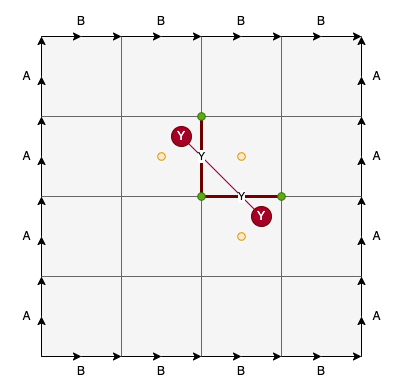
\includegraphics[scale=0.30]{Y-type}
\caption{Movement of $Y$-type particles in toric code}
\label{fig:Y-type}
\end{center}
\end{figure}

To write out the full set of fusion rules for the toric code, we need one last particle type. Namely, the ``do-nothing" particle that one gets when fusing a particle with its own antiparticle. While physically trivial, this particle is neccecary to make our mathematical descriptions. Seeing as the do-nothing particle moves by doing nothing, we call it the $I$-type particle since it moves by tensoring with $I$. We denote $a\otimes b$ for the fusion of two particles $a$ and $b$. It will become clear in the category theoretic notation why the tensor product symbol is used. The fusion rules are given as a table below:

\begin{center}
\begin{tabular}{c |c |c |c |c} 
  & $I$ & $X$ & $Y$ & $Z$ \\ [0.5ex] 
 \hline
 $I$ & $I$ & $X$ & $Y$ & $Z$ \\ 
 \hline
 $X$ & $X$ & $I$ & $Z$ & $Y$ \\
 \hline
 $Y$ & $Y$ & $-Z$ & $I$ & $X$ \\
 \hline
 $Z$ & $Z$ & $-Y$ & $-X$ & $I$
\end{tabular}
\end{center}

We make a few observations. The fact that $X$ fused with $Z$ is $Y$ is by definition. The fact that $Z$ and $X$ fuse to $-Y$ comes from the fact that fusing the opposite direction means applying $\sigma_Z\sigma_X$ to the edge instead of $\sigma_X\sigma_Z$. Seeing as $\sigma_X$ and $\sigma_Z$ anticommute, this gives a $-1$ sign. All of the other boxes in the table can be checked similarly. For example, $Z\otimes Y=-X$ becasue $\sigma_Z(i\sigma_Y)=-\sigma_X$. We observe that fusion essentially gives a group law on the space of anyon types. However, this is not exactly the case: Sometimes the output is positive, and sometimes the output is negative.

In general, fusion will have the following structure. We let $\LL$ be a finite set, which we think of as being the possible anyon types. For any $a,b\in \LL$, we will have the formal equality

$$a\otimes b=\sum_{c\in \LL}N_{c}^{a,b}c.$$

This formula intuitively says that when $a$ and $b$ are fused this will result in a collection of particles, constisting of $N_c^{a,b}$ copies of $c$ for each $c\in \LL$. This can be thought of as the generalization of a finite group, where now the group law is allowed to output formal linear combinations of elements in the group. These generalizations of groups are called \textit{fusion systems}. Those fusion systems which satisfy a generalization of commutivity are called \textit{braided fusion systems}, and correspond to braided fusion categories. Modular Tensor Categories are braided fusion categories which satisfy a certain non-degeneracy and symmetry condition. In this way, one can think of MTCs as being vast ``non-degenerate" generalizations of finite abelian groups. We now formally state the definition of fusion system:


\begin{definition}[Fusion system] A fusion system is the following data.

\begin{enumerate}
\item (Anyon types) A finite set $\LL$.
\item (Fusion coefficients) Integers $N_{c}^{a,b}\in\{0,1\}$ for all $a,b,c\in \LL$.
\end{enumerate}

Additionally, a fusion system is required to satisfy the following properties:

\begin{enumerate}
\item (Identity/Do-nothing) There is a unique element $1\in \LL$ such that

$$1\otimes a=a\otimes 1=a$$

for all $a\in \LL$. In other words,

$$N^{a,1}_{b}=N^{1,a}_{b}=\begin{cases}1 & a=b \\ 0 & \text{otherwise}\end{cases}$$

for all $a,b\in \LL$.

\item (Inverse/anti-particle) There is a unique element $a^*\in \LL$ such that

$$a\otimes a^*=1\oplus [\text{other terms}],$$

for all $a\in \LL$. For all  $b\neq a^*$, $a\otimes b$ has no $1$ term. In other words,

$$N^{a,b}_{1}=N^{b,a}_{1}=\begin{cases} 1 & b=a^* \\ 0 & \text{otherwise}\end{cases}$$

for all $a, b\in \LL$.

\item (Associativity) We have

$$(a\otimes b)\otimes c=a\otimes (b\otimes c)$$

for all $a,b,c\in \LL$. In other words, for all $a,b,c,d\in \LL$ we have that

$$\sum_{e\in \LL}N_e^{a,b}N_{d}^{e,c}=\sum_{e\in \LL}N_{e}^{b,c}N_d^{a,e}.$$
\end{enumerate}

\raggedleft\qedsymbol{}
\end{definition}

Observe that in the above definition we required that $N_c^{a,b}$ always be $0$ or $1$. That is, when two particles are fused they will not create multiple copies of the same particle. This condition is not strictly neccecary, but we included it here as it greatly simplifies the theory. Many authors do not put this stipulation, and refer to examples with $N_c^{a,b}$ always equal to $0$ or $1$ as multiplicity free. 

The next piece of the puzzle is based on one of the key ideas from category theory: Equal versus isomorphic. Given quasiparticles $a,b,c$ fusing via $(a\otimes b)\otimes c$ or $a\otimes (b\otimes c)$ will result in the same particles. However, just because the particles present are the same does not mean that the quantum systems are the same. A huge theme in Section \ref{The Toric Code} is that changing order in processes like braiding might result in the same particles, but different states. Namely, different states in the same eigenspace. The processes $(a\otimes b)\otimes c$ and $a\otimes(b\otimes c)$ need only be equal up to an invertable linear transformation, i.e., isomorphism. We will define a $6j$ fusion system to be a fusion system in which we have chosen isomorphisms between all $(a\otimes b)\otimes c$ and $a\otimes (b\otimes c)$.

The visualization of this is best suited to a graphical language. As we will see next section, it is really best suited to a category-theoretic graphical language. The idea behind the graphical language is to make rigorous the sorts of diagrams that one will obviously draw when explaining the subject, as to clarify often messy conditions one will impose on objects. The general policy for these diagrams is as follows.

\begin{enumerate}
\item The diagrams are to be read from top to bottom.
\item Strands correspond to anyons.
\item Operations on strands correspond to operations on anyons.
\end{enumerate}

\begin{figure}
\begin{center}
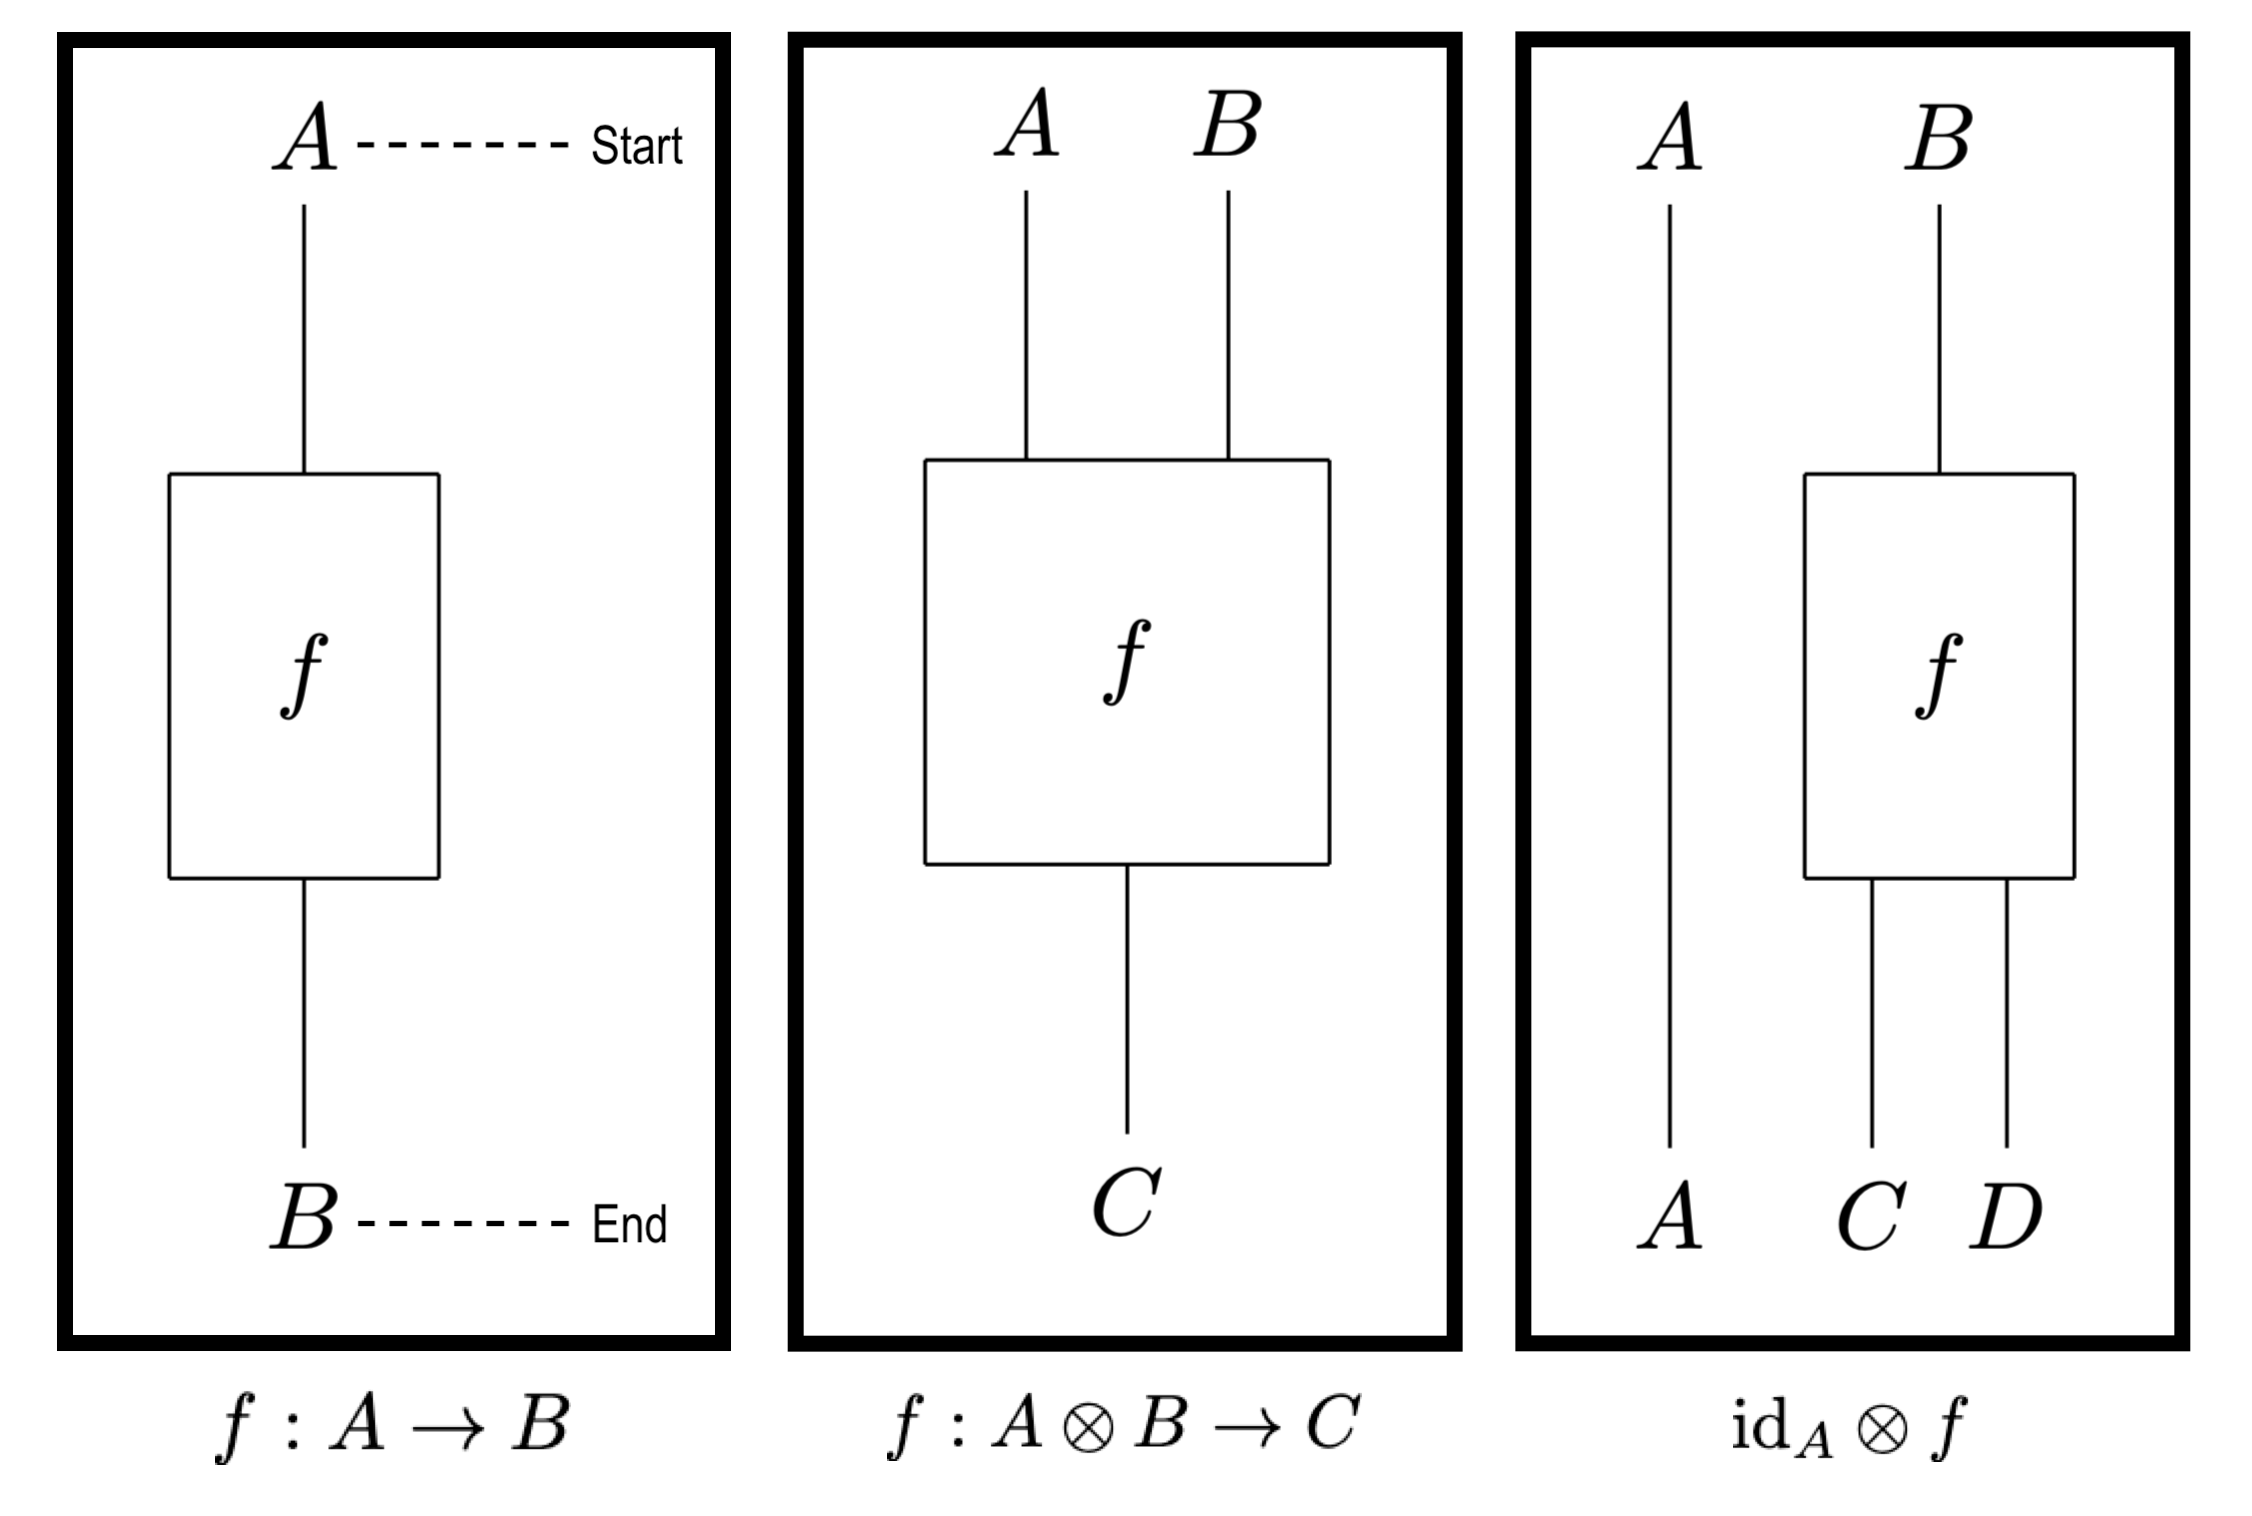
\includegraphics[scale=0.2]{graphical-language}
\caption{Examples of the quantum algebraic graphical language}
\label{fig:graphical-language}
\end{center}
\end{figure}

Some examples can be found in Figure \ref{fig:graphical-language}. Some special functions are encoced via special graphical diagrams. For example, suppose we choose a distinguished function $a\otimes b\to c$ to represent $a\otimes b$ fusing into $c$. In general the choice is mostly arbitrary, and changing our choices of such functions is \textit{gauge symmetry}, as will be formally defined later. Our informal notion of function will be put in firmer footing in Subsection \ref{Category viewpoint} when we use category theory. We graphically write our distinuished function $a\otimes b\to c$ as

\begin{equation*}
  \tikzfig{simple-cotriangle}
\end{equation*}

Consider a function $(a\otimes b)\otimes c \to d$. This can be decomposed as taking a function $a\otimes b\to n$, then $n\otimes c\to d$, i.e., as

$$(a\otimes b)\otimes c\to n\otimes c\to d.$$

Similarly, functions $a\otimes (b\otimes c)\to d$ can decomposed by taking functions $b\otimes c\to m$ and $a\otimes m\to d$. These two processes can be represented in terms of each other by a linear combination. In the graphical language, this is expressed as

\begin{equation*}
  \tikzfig{6j-tree}
\end{equation*}

These values $F^{a,b,c}_{d;n,m}\in \CC$ are known as $6j$ symbols. They clearly depend on the choice of functions ($a\otimes b\to n$ and such). Understanding the real intuition behind these $6j$ symbols without any handwaiving will have to wait until next section. However, for our purposes, this is really not neccecary: These can be treated simply as complex numbers, with as much or as little intuition behind them as one desires. All that is required is that they satisfy some axioms, as in the following definition:

\begin{definition}[$6j$ Fusion system] A $6j$ fusion system is the following data.

\begin{enumerate}
\item A fusion system $(\LL, N_{\--}^{\--,\--})$
\item Complex numbers $F^{a,b,c}_{d;n,m}$ for all $a,b,c,d,n,m\in \LL$.
\end{enumerate}

Additionally, a $6j$ fusion system is required to satisfy the following properties:

\begin{enumerate}

\item (Admissibility) We call a triple $(a,b,c)\in \LL^3$ admissible if $N^{a,b}_c\neq 0$. We call a sextuple $(a,b,c,d,n,m)\in \LL^6$ admissible if $(a,b,m)$, $(m,c,d)$, and $(b,c,n)$ are all admissible. We write $F^{a,b,c}_{d}$ to be the matrix whose coefficients are $F^{a,b,c}_{d;n,m}$, where $n,m$ run over pairs making $(a,b,c,d,n,m)$ admissible. We have that
\begin{itemize}
\item $F^{a,b,c}_{d;n,m}=0$ if $(a,b,c,d,n,m)$ is not admissible
\item $F^{a,b,c}_{d}$ is invertible
\end{itemize}

for all $a,b,c,d,n,m$.

\item (Associativity trivial on two inputs) $F^{a,b,c}_{d}$ is the identity matrix, whenever one of $a$, $b$, or $c$ is $1$.

\item (Pentagon) For all $a,b,c,d,e,f,p,q,m\in\LL$,

$$\sum_{n\in \LL}F^{b,c,d}_{q;p,n}F^{a,n,d}_{f;q,e}F^{a,b,c}_{e;n,m}=F^{a,b,p}_{f; q,m}F^{m,c,d}_{f;p,e}.$$

\item (Time reversal symmetry) $\left[\left(F^{a^*,a,a^*}_{a^*}\right)^{-1}\right]_{1,1}=\left[F^{a,a^*,a}_{a}\right]_{1,1}$, where $\left[\cdot\right]_{n,m}$ denotes the $[n,m]$th entry of a matrix.
\end{enumerate}
\raggedleft\qedsymbol{}
\end{definition}

Seeing as these axioms are more complicated, we explain them all in detail. Admissibility of the triple $(a,b,c)$ says that when $N^{a,b}_{c}\neq 0$, which is equivilant to saying that when $a$ and $b$ fuse, a $c$ particle is created. In the language of functions, this is saying that there is a nonzero map $a\otimes b\to c$, i.e., a nonzero physical process taking as input $a\otimes b$ and outputting $c$.  Thus, when we think about decomposing $a\otimes b\otimes c$ as maps $a\otimes b\to n$, $m\otimes c\to d$, and $b\otimes c\to n$, it makes sense that if any of these pairs is not admissible then $F^{a,b,c}_{d;n,m}=0$. One of those tripes being nonadmissible would mean that one of the functions in one of the compositions $a\otimes b\otimes c\to d$ is $0$, and hence the function itself is zero, and hence will contribute nothing to the change of basis. Similarly, the matrix $F^{a,b,c}_{d}$ should give an equivilance between functions $(a\otimes b)\otimes c \to d$ and functions $a\otimes (b\otimes c)\to d$. Equvilance means isomorphism, which means that $F^{a,b,c}_{d}$ should be invertible.

If one of $a,b,c$ is $1$, then $F^{a,b,c}_{d}$ should surely be the identity. Imagine, for instance, $c=1$. Then, we will be relating $(a\otimes b)\otimes 1$ and $a \otimes (b\otimes 1)$. Tensoring with $1$ should not only leave you isomorphic with where you started, but it should really leave you equal. That is, we should be able to suppress $\otimes 1$ from notation and things should still work. Upon removing the $\otimes 1$, we find that we are relating $a\otimes b$ and $a\otimes b$, two equal objects, and hence the transformation $F^{a,b,c}_{d}$ should be the identity.

The pentagon identity is exactly the sort of identity for which graphical language is useful. As stated, it is quite non-obvious to decipher meaning from the expression. It becomes the statement that applying associativity in two diffent ways is identical. In graphical language, it becomes the fact that going either way around the 5-term diagram in Figure \ref{fig:pentagon} gives the same answer (hence the name pentagon). All of terms in the pentagon are maps $a \otimes b\otimes c\otimes d \to e$. Each of the arrows corresponds to applying the approproate $F$-matrix.



\begin{figure}
\begin{center}
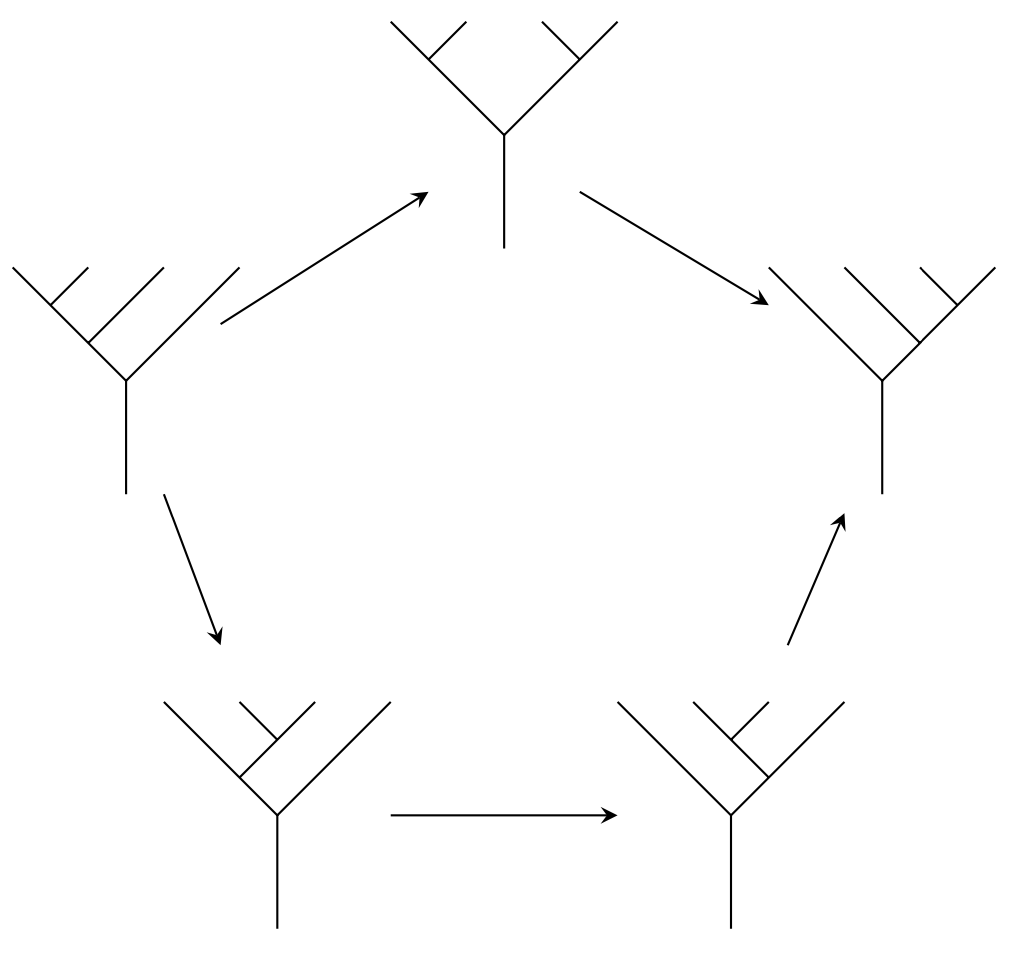
\includegraphics[scale=0.28]{pentagon}
\caption{The pentaon axiom for $6j$ symbols}
\label{fig:pentagon}
\end{center}
\end{figure}


[WORK: Explain time reversal symmetry]

A natural question about the definition of $6j$ symbols could be as follows: The goal was to define an isomorphism $a\otimes (b\otimes c)$ to $(a\otimes b)\otimes c$. Instead, one defined how morphisms $a\otimes (b\otimes c)\to d$
 and $(a\otimes b)\otimes c\to d$ relate for every $d$. While this does indeed give some connection between $a\otimes (b\otimes c)$ and $(a\otimes b)\otimes c$, it is not immediately clear that tells us the two objects are isomorphic or, if so, what that isomorphism would be. While seemingly counterintuitive, this switch from studying objects to studying the functions between objects is extremely fruitful. This forms the heart of the Yoneda lemma, the most important result in category theory: Objects should be understood by their relationship with each other. According to Ravi Vakil:

\begin{quote}
You work at a particle accelerator. You want to understand some particle. All you can do are throw other particles at it and see what happens. If you understand how your mystery particle responds to all possible test particles at all possible test energies, then you know everything there is to know about your mystery particle - Ravi Vakil\footnote{This quote is folklore, relayed by a MathOverflow post of Theo Johnson-Freyd}.
\end{quote}

In this context, Vakil's quote is very literal - we are studying particles by looking at their fusion rules. Fusion, as a process, generally happens when things hit each other very fast in a particle accelerator. By knowing that $a\otimes (b\otimes c)$ and $(a\otimes b)\otimes c$ can go to $d$ in all the same ways (with the relationship being those ways being specified by the matrix $F^{a,b,c}_d$), we can conclude an isomorphism between $a\otimes (b\otimes c)$ and $(a\otimes b)\otimes c$. A formal treatment of the Yoneda lemma insofar as it relates to our study is given in the next section.

We now define braided $6j$ fusion systems. A braiding should give the relashionship between $a\otimes b$ and $b\otimes a$. These objects will be isomorphic, but not equal. For example, the fact that $X$ and $Z$ anticommute in the toric code is exactly the statement that isomorphism $X\otimes Z\to Z\otimes X$ should be $-1$ times the identity. Keeping with our Yoneda perspective, instead of giving an isomorphism $a\otimes b$ and $b\otimes a$ we give isomorphism between the spaces $a\otimes b\to c$ and $b\otimes a\to c$ for every $c$. Graphically, this can be seen in Figure [WORK: make figure]. The formal definition is as follows:

\begin{definition}[Braided $6j$ Fusion system] A braided $6j$ fusion system is the following data.

\begin{enumerate}
\item A $6j$ fusion system $(\LL, N_{\--}^{\--,\--},F^{\--,\--,\--}_{\--;\--,\--})$.
\item Complex numbers $R^{a,b}_{c}$ for all $a,b,c\in \LL$.
\end{enumerate}

Additionally, a braided $6j$ fusion system is required to satisfy the following properties:

\begin{enumerate}

\item (Admissibility) $R^{a,b}_{c}\neq 0$ if $(a,b,c)\in \LL^3$ is admissible

\item (Hexagon) For all $a,b,c,d,e,m\in\LL$,

$$\left(R^{a,c}_{e}\right)^{\pm 1}F^{b,a,c}_{d;e,m}\left(R^{a,b}_{m}\right)^{\pm 1}=\sum_{n\in \LL} F^{b,c,a}_{d;e,n}\left(R^{a,n}_{d}\right)^{\pm 1}F^{a,b,c}_{d;n,m}.$$
\end{enumerate}
\raggedleft\qedsymbol{}
\end{definition}

Again, the hexagon is a mess of symbols when written out explicitely. In graphical language, we can [WORK: what does braiding look like]. The hexagon identity is thus the condition that going either way around the following 6-term diagram gives the same answer:

[WORK: Make hexagon]

With all this, we can finally define an MTC:

\begin{definition}[Modular tensor fusion system] A modular tensor fusion system is a braided $6j$ fusion system satsifying the following conditions

\begin{enumerate}

\item (Spherical) $F^{a,b,c}_{1;a^*,c}F^{b,c^*,a}_{1;a^*a,a}F^{c^*,a,b}_{1;b^*,b}=1$ for all $a,b,c\in \LL$.

\item (Non-degenerate) For $a\in \LL$, if $B_c^{a,b}=B_c^{b,a}$ for all $b,c\in \LL$, then $a=1$.
\end{enumerate}
\raggedleft\qedsymbol{}
\end{definition}

In graphical language, the spherical condition looks like [WORK: make diagram, explain why its neccecary.]

The non-degeneracy condition says that every non-trival particle should braid non-trivially with at least one other particle. Graphically, this is shown in [WORK: make diagram].

It is important to remember that even though the definition is long, at the end of the day these are still just finite collections of numbers satisfying a finite number of polynomial equations. This makes many things simple. For instance, we can define a morphism between fusion systems $(\LL,N)$ and $(\LL',N')$ to be a function $f:\LL\to \LL'$ such that $N^{a,b}_{c}=N'^{f(a),f(b)}_{f(c)}$. For $6j$ fusion sytems and braided $6j$ fusion systems, we simply require that $f$ should respect $F$ symbols and $R$ symols as well. We can thus properly speak of fusion systems up to equivilance. We will see in the next section, however, that the correct notion of equivilance is a weaker \textit{gauge equivilance}. This corresponds to keeping the same label set, but performing a local change of basis on $F$ matricies.

\begin{definition}[Gauge equivilance of $6j$ symbols] A gauge equivilance of $6j$ symbols $F^{\--,\--,\--}_{\--}$ and $\tilde{F}^{\--,\--,\--}_{--}$ on a fusion sytem $(\LL,N^{\--,\--}_{\--})$ is the following data:

\begin{enumerate}
\item Complex numbers $f^{a,b}_{c}$ for all $a,b,c\in \LL$.
\end{enumerate}

Additionally, a gauge equivilance of $6j$ symbols is required to satisfy the following properties:

\begin{enumerate}
\item $f^{a,b}_{c}\neq 0$ if and only if $(a,b,c)\in \LL^3$ is admissible.
\item $f^{1,a}_{a}=f^{a,1}_{a}=1$ for all $a\in \LL$.
\item (Rectangle axiom) For all $a,b,c,d,n,m\in \LL$,

$$f_n^{b,c}f^{a,n}_{d}F^{a,b,c}_{d;n,m}=\tilde{F}^{a,b,c}_{d;n,m}f^{a,b}_{m}f^{m,c}_{d}.$$
\end{enumerate}
\raggedleft\qedsymbol{}
\end{definition}

If $(\LL,N,F)$ and $(\LL',N',F')$ are $6j$ fusion systems with different label sets, then a gauge equivilance between $\LL$ and $\LL'$ is a guage equivilance of $(\LL,N,F)$ to some system $(\LL,N,\tilde{F})$, followed by a standard equivilance of fusion systems between $(\LL,N,\tilde{F})$ and $(\LL',N',F')$.

.[WORK: Give explination of rectangle axiom, preferably with graphical language]

In the case of the toric code we summarize the relevant data. The label set is $\LL=\{I,X,Y,Z\}$. The nonzero fusion coefficients are given by

\begin{center}
\begin{tabular}{c |c |c |c |c} 
  & $I$ & $X$ & $Y$ & $Z$ \\ [0.5ex] 
 \hline
 $I$ & $N^{I,I}_{I}=1$ & $N^{I,X}_{X}=1$ & $N^{I,Y}_{Y}=1$ & $N^{I,Z}_{Z}=1$ \\ 
 \hline
 $X$ & $N^{X,I}_{X}=1$ & $N^{X,X}_{I}=1$ & $N^{X,Y}_{Z}=1$ & $N^{X,Z}_{Y}=1$ \\
 \hline
 $Y$ & $N^{Y,I}_{Y}=1$ & $N^{Y,X}_{Z}=1$ & $N^{Y,Y}_{I}=1$ & $N^{Y,Z}_{X}=1$ \\
 \hline
 $Z$ & $N^{Z,I}_{Z}=1$ & $N^{Z,X}_{Y}=1$ & $N^{Z,Y}_X=1$ & $N^{Z,Z}_I=1$
\end{tabular}
\end{center}

All of the $F$ matricies are the identity. The non-unit non-zero braiding coefficients are given by

\begin{center}
\begin{tabular}{c |c |c |c |c} 
  & $I$ & $X$ & $Y$ & $Z$ \\ [0.5ex] 
 \hline
 $I$ & & &  &  \\ 
 \hline
 $X$ & &  & $R^{X,Y}_{Z}=-1$ & $R^{X,Z}_{Y}=-1$ \\
 \hline
 $Y$ &  & $R^{Y,X}_{Z}=-1$ & & $R^{Y,Z}_{X}=-1$ \\
 \hline
 $Z$ &  & $R^{Z,X}_{Y}=-1$ & $R^{Z,Y}_X=-1$ & 
\end{tabular}
\end{center}

This gives a full definition of the toric code as modular tensor fusion system. All that is left is to show is that all of the axioms of are satisfied - this is Exercise \thesection.3.


\subsection{The category-theoretic viewpoint}
\label{Category viewpoint}

In this subsection, we give the category theoretic perspective on Modular Tensor Categories (MTCs). As with subsection \ref{Anyon model}, we will build up to the definition of a MTC slowly. Thinking of MTCs as corresponding to ``non-degenerate" finite abelian groups, we will start with the category-theory analogues of monoids\footnote{A monoid is a set equipped with an associative binary operation and an identity element}, groups, finite groups, finite abelian groups, and then end with non-degenerate finite abelian group. The category theory analogues are as below:

\begin{center}
\begin{tabular}{c ||c } 
  
Algebraic structure & Categorification \\
\hline
\hline
Set & Category \\ 
 \hline
Monoid & Monoidal category\\
 \hline
Finite group &  Fusion category\\
 \hline
Finite abelian group & Braided fusion category \\
\hline
``non-degenerate" finite abelian group & Modular Tensor Category  
\end{tabular}
\end{center}
. We begin with the generalization of monoid:

\begin{definition}[Monoidal category] A monoidal category is the following data:

\begin{enumerate}
\item A category $\Ccat$.
\item A functor $\otimes: \Ccat \times \Ccat \to \Ccat$.
\item (Identity) A distinguished element $1\in \Ccat.$
\item (Associativity) A natural equivilance $\alpha: \--\otimes (\-- \otimes \--) \to (\--\otimes \--)\otimes \--$, where $\-- \otimes (\--\otimes \--)$ denotes the functor $\Ccat\times \Ccat\times \Ccat\to\Ccat$ sending $(A,B,C)$ to $A\otimes (B\otimes C)$, and similarly for $(\-- \otimes \-- )\otimes\--$.
\item (Left unitor) A  natural equivilance $\lambda: 1\otimes \-- \to \--$, where $1\otimes \--$ denotes the functor $\Ccat\to \Ccat$ sending $A$ to $1\otimes A$, and $\--$ denotes the identity.
\item (Right unitor) A natural equivilance $\rho: \--\otimes 1 \to \--$, where $\--\otimes 1$ is the functor $\Ccat\to \Ccat$ sending $A$ to $A\otimes 1$.
\end{enumerate}

Additionally, a monoidal category is required to satisfy the following properties:

\begin{enumerate}
\item (Triangle identity) For all $A,B\in \Ccat$, the diagram

\[\begin{tikzcd}
	{} & {} & {\left(A\otimes 1\right)\otimes B} & {} & {A\otimes (1\otimes B)} \\
	&& {} & {A\otimes B} \\
	&&&& {}
	\arrow["{\alpha_{A,1,B}}", from=1-3, to=1-5]
	\arrow["{\rho_A\otimes \text{id}_B}"', from=1-3, to=2-4]
	\arrow["{\text{id}_A\otimes \lambda_B}", from=1-5, to=2-4]
\end{tikzcd}\]

commutes.

\item (Pentagon identity) For all $A,B,C,D\in \Ccat$, the diagram

\[\begin{tikzcd}
	& {(A\otimes B)\otimes(C\otimes D)} \\
	{((A\otimes B)\otimes C)\otimes D} && {A\otimes (B\otimes (C\otimes D))} \\
	{(A\otimes (B\otimes C))\otimes D} && {A\otimes((B\otimes C)\otimes D)}
	\arrow["{\alpha_{A\otimes B, C,D}}", from=2-1, to=1-2]
	\arrow["{\alpha_{A,B,{C\otimes D}}}"', from=2-3, to=1-2]
	\arrow["{\alpha_{A,B,C}\otimes \text{id}_D}"', from=2-1, to=3-1]
	\arrow["{\text{id}_A\otimes_{B,C,D}}"', from=3-3, to=2-3]
	\arrow["{\alpha_{A,B\otimes C,D}}"', from=3-1, to=3-3]
\end{tikzcd}\]

commutes.
\end{enumerate}

\raggedleft\qedsymbol{}
\end{definition}

Observe the parallels between the propreties of monoidal categories and the prerties of $6j$ fusion systems. The triangle identity can be seen as analagous to the fact that associativity being trivial on two inputs, and the pentagon is analagous to the pentagon. We will make this explicit when we show how to make fusion systems from categories.

In the definition of fusion systems, the identity, associativity, and inverse are properties instead of structures. They are unique if they exist. While the identity will be unique up to isomorphism, one still must make a choice of object. There are possibly multiple different choices of natural equivilances for the unit. In category theory, the difference between equal and isomorphic is very pronounced, and one needs to choose an isomorphism. The following theorem answers in what sense we really do get mileage out of considering categories in which we make strange choices of $\alpha,\lambda,\rho$, and in what sense we really do get mileage out of considering categories with multiple objects in the same equivilance class. The notion of monoidal equivilance is used in the theorem; we postpone the definition until after the statement.

\begin{theorem}[\cite{hagge2009some}] Let $(\Ccat,\otimes_{\Ccat},\alpha_{\Ccat},\lambda_{\Ccat},\rho_{\Ccat})$ be a monoidal category. Then

\begin{enumerate}
\item (MacLane)  $\Ccat$ is monoidally equivilant to a category $(\Dcat,\otimes_{\Dcat},\alpha_{\Dcat},\lambda_{\Dcat},\rho_{\Dcat})$ in which $A\otimes_{\Dcat} (B\otimes_{\Dcat} C)=(A\otimes_{\Dcat} B)\otimes_{\Dcat} C$, $1\otimes_{\Dcat} A=A\otimes_{\Dcat} 1=1$, and $\alpha_{\Dcat},\lambda_{\Dcat},\rho_{\Dcat}$ are identity functors, for all $A,B,C\in \Dcat$. 
\item $\Ccat$ is monoidally equivilant to a category in $\Dcat$ in which all objects which are isomorphic are equal.
\end{enumerate}

However, $\Ccat$ is \textbf{not} in general equivilant to a category which is both at the same time.
\end{theorem}

This theorem really says that you cannot have your cake and eat it too. You can forget about non-trivial maps or you can forget about non-equal isomorphic obects, but you can't do both at once. Authors will often assume either one condition or the other (known as \textit{strict} and \textit{skeletal} respectively), and this will sometimes lead to confusion across the literature. A monoidal equivilance is a monoidal functor which has an inverse.

\begin{definition}[Monoidal functor] A monoidal functor between monoidal categories $(\Ccat,\otimes_{\Ccat}, \alpha_{\Ccat},\lambda_{\Ccat},\rho_{\Ccat},1_{\Ccat})$ and $(\Dcat,\otimes_{\Dcat},\alpha_{\Dcat},\lambda_{\Dcat},\rho_{\Dcat},1_{\Dcat})$ is the following data:

\begin{enumerate}
\item A functor $F: \Ccat\to \Dcat$.
\item A morphism $\epsilon:1_{\Dcat}\to F(1_{\Ccat})$.
\item A natural transformation $\mu$ between the functors $F(\--)\otimes_{\Dcat}F(\--)$ and $F(\--\otimes_{\Ccat}\--)$.
\end{enumerate}

Additionally, a monoidal functor is required to satisfy the following properties:

\begin{enumerate}
\item (Associativity) For all $A,B,C\in \Ccat$, the diagram

\[\begin{tikzcd}
	{(F(A)\otimes_{\Dcat}F(B))\otimes_{\Dcat}F(C)} &&& {F(A)\otimes_{\Dcat}(F(B)\otimes_{\Dcat}F(C))} \\
	{F(A\otimes_{\Ccat}B)\otimes_{\Dcat}F(C)} &&& {F(A)\otimes_{\Dcat}F(B\otimes_{\Ccat}C)} \\
	{F((A\otimes_{\Ccat} B)\otimes_{\Ccat}C)} && {} & {F(A\otimes_{\Ccat}B\otimes_{\Ccat}C)}
	\arrow["{\mu_{A,B}\otimes \text{id}_{F(C)}}", from=1-1, to=2-1]
	\arrow["{\mu_{A\otimes_{\Ccat}B,C}}", from=2-1, to=3-1]
	\arrow["{\mu_{A,B\otimes_{\Ccat}C}}", from=2-4, to=3-4]
	\arrow["{\text{id}_{F(A)}\otimes\mu_{B,C}}", from=1-4, to=2-4]
	\arrow["{F(\alpha_{\Ccat;A,B,C})}"{description}, from=3-1, to=3-4]
	\arrow["{\alpha_{\Dcat;F(A),F(B),F(C)}}"{description}, from=1-1, to=1-4]
\end{tikzcd}\]

commutes.
\item (Unitality) The diagrams

\[\begin{tikzcd}
	{1_{\Dcat}\otimes_{\Dcat}F(A)} && {F(1_{\Ccat})\otimes F(A)} \\
	{F(A)} && {F(1_{\Ccat}\otimes A)}
	\arrow["{\lambda_{\Ccat;F(A)}}", from=1-1, to=2-1]
	\arrow["{F(\lambda_{\Ccat;A})}"', from=2-3, to=2-1]
	\arrow["{\mu_{1_{\Ccat},A}}"', from=1-3, to=2-3]
	\arrow["{\epsilon\otimes \text{id}_{F(A)}}"', from=1-1, to=1-3]
\end{tikzcd}\]

and

\[\begin{tikzcd}
	{F(A)\otimes_{\Dcat}1_{\Dcat}} && {F(A)\otimes_{\Dcat}F(1_{\Ccat})} \\
	{F(A)} && {F(1_{\Ccat}\otimes A)}
	\arrow["{\rho_{\Ccat;F(A)}}", from=1-1, to=2-1]
	\arrow["{F(\rho_{\Ccat;A})}"', from=2-3, to=2-1]
	\arrow["{\mu_{A,1_{\Ccat}}}"', from=1-3, to=2-3]
	\arrow["{\text{id}_{F(A)}\otimes\epsilon}"', from=1-1, to=1-3]
\end{tikzcd}\]

commute for all $A\in \Ccat$.
\end{enumerate}

\raggedleft\qedsymbol{}
\end{definition}

We now define fusion categories. One key difficulty is deciding what category-theorertical object should correspond to the label set $\LL$ of a fusion system. The answer is as follows. We want general elements of $\Ccat$ to be uniquely representable as direct sums of the elements in the label set. The elements of $\Ccat$ which cannot be broken down further as direct sums of smaller objects are known as indecomposable objects.

There are a few difficulties in trying to formalize this idea. For one, you might be in the strange case that there are indecomposable objects that still have smaller subjects. For example, consider the category of abelian groups. The group $\ZZ_4$ has the subject $\ZZ_2$. However, $\ZZ_2\oplus\ZZ_2\neq \ZZ_4$. Formally, this example is saying that the exact sequence

$$0\to \ZZ_2\to \ZZ_4\to\ZZ_2\to 0$$

does not split. An introduction to exact sequences is found in Appendix \ref{Categories}. What we really want is that every object should be the direct sum of objects which themselves have no subjects. Objects with no subobjects are called irriducible objects. This discrepency between irriducible and indecomposable forms one of the key themes of representation theory, and leads to a great deal of subtledy. Irrididucible objects are also called simple objects. Categories in which there is no discrepency between irrididuble and indecomposable are called semisimple, i.e., semisimple categories are those categories in which every object is the direct sum of simple objects.

This discussion above strongly uses the notion of \textit{subobject}. However, it is not clear in general what subobject should mean. The classic intuation is that $A$ is a subobject of $B$ if there is an injective map $f:A\hookrightarrow{}B$. Being injective is the statement that the kernel of $f$ is  $0$, but in arbitarary categories there is no good notion of kernel. Thus, we restrict our attention to \textit{abelian} categories. Being abelian comes with a large amount of desirable properties, and most categories people consider are abelian. In abelian categories, we require that all hom sets are given the structure of abelian groups. This is done for various reasons [WORK: what are those reasons?]. Seeing as our eyes are towards quantum physics, all hom sets will be $\CC$ vector spaces. Linear combinations of morphisms will correspond to superpositions. To preserve space, we combine ``abelian" and ``$\CC$-linear" into one definition:

\begin{definition}[$\CC$-linear abelian category]  A $\CC$-linear abelian category is the following data:

\begin{enumerate}
\item A category $\Ccat$.
\item The structure of a $\CC$ vector space on $\Hom(A,B)$ for all $A,B\in \Ccat$.
\end{enumerate}

Additionally, a semisimple linear category is required to satisfy the following properties:

\begin{enumerate}
\item (Linearity) The composition map $\Hom(A,B)\times \Hom(B,C)\to \Hom(A,C)$ is bilinear for all $A,B,C\in \Ccat$.
\item (Has a zero object) There is an object $0\in \Ccat$ such that for every $A\in \Ccat$ there is a unique morphism $0\to A$.
\item (Has binary biproducts) For all $A,B\in \Ccat$ the biproduct of $A$ and $B$ exists. This biproduct is denoted $A\oplus B$, and refered to as the direct sum. Recall that the biproduct of $A$ and $B$ is an object $A\oplus B$, paired with morphisms $p_{A},p_{B}: A\oplus B\to A,B$, and  $i_{A},i_{B}: A,B\to A\oplus B$, such that

\begin{itemize}
\item $p_{X}\circ i_{Y}$ is $\text{id}_X$ when $X=Y$, and $0$ otherwise,
\item $i_{A}\circ p_{A}+i_{B}\circ p_{B}=\text{id}_{A\oplus B}$.
\end{itemize}
\item (Has kernels and cokernels) For all $A,B\in \Ccat$ and $f:A\to B$, we have objects $\ker f, \coker f$, and morphisms $i:\ker f\to A$, $p: B\to \coker f$. We require that

\begin{itemize}
\item $f\circ i=0$.
\item For any $i': \ker' f\to A$ with $f\circ i'=0$, there is a morphism $u: \ker'f\to \ker f$ such that

\[\begin{tikzcd}
	& A \\
	& {\ker f} & B \\
	{\ker' f}
	\arrow["f", from=1-2, to=2-3]
	\arrow["{i'}", from=3-1, to=1-2]
	\arrow["0"', from=3-1, to=2-3]
	\arrow["i"', from=2-2, to=1-2]
	\arrow["0", from=2-2, to=2-3]
	\arrow["u"{description}, dashed, from=3-1, to=2-2]
\end{tikzcd}\]

commutes.

\item $p\circ f=0$
\item For any $p':B\to \coker' f$ with $p'\circ f=0$, there is a morphism $u: \coker f\to \coker' f$ such that

\[\begin{tikzcd}
	& A \\
	& {\coker f} & B \\
	{\coker' f}
	\arrow["f", from=1-2, to=2-3]
	\arrow["0"', from=1-2, to=3-1]
	\arrow["{p'}", from=2-3, to=3-1]
	\arrow["0"', from=1-2, to=2-2]
	\arrow["p"', from=2-3, to=2-2]
	\arrow["u"{description}, dashed, from=2-2, to=3-1]
\end{tikzcd}\]

commutes
\end{itemize}
\item (All monomorphisms and epimorphisms are normal) All monomorphisms are kernels, and all epimorphisms are cokernels. A monomorphism $f:A\to B$ is a map such that for all $g_0,g_1: C\to A$, $f\circ g_0=f\circ g_1$ if and only if $g_0=g_1$. A monomorphism is said to be normal if it is the kernel of some morphism. An epimorphism $f:A\to B$ is a map such that for all $g_0,g_1:B\to C$, $g_0\circ f=g_1\circ f$ if and only if $g_0=g_1$. An epimorphism is said to be normal if it is the cokernel of some morphism.


\end{enumerate}
\raggedleft\qedsymbol{}
\end{definition}

A general $\CC$-linear category is a $\CC$-linear abelian category which only needs to satisfy the linearity condition. As always, when defining an object one must define the appropriate morphisms:

\begin{definition}[$\CC$-linear functor] A $\CC$-linear is a functor between $\CC$-linear categories $\Ccat,\Dcat$ is a functor $F:\Ccat\to\Dcat$ such that $F:\Hom(A,B)\to \Hom(F(A),F(B))$ is a linear map of vector spaces for all $A,B\in \Ccat$.
\end{definition}

Will these definitions out of the way, we can now define fusion categories.

\begin{definition}[Fusion category]  A fusion category is the following data:

\begin{enumerate}
\item A $\CC$-linear abelian monoidal category $\Ccat$.
\item (Duals) Choices of objects $A^*$ for every object $A\in \Ccat$.
\item (Unit/co-unit)Choices of morphisms $\eta_A: 1\to A^*\otimes A$ and $\epsilon_A: A\otimes A^*\to 1$ for all $A\in \Ccat$
\end{enumerate}

Additionally, a fusion category is required to satisfy the following properties:

\begin{enumerate}
\item The tensor product, associativity, left unitor, and right unitor of $\Ccat$ are all $\CC$-linear functors.
\item (Rigidity) The diagrams

\[\begin{tikzcd}
	{A\otimes (A^*\otimes A)} && {(A\otimes A^*)\otimes A} \\
	& A
	\arrow["{\epsilon_A\otimes \text{id}_A}", from=1-3, to=2-2]
	\arrow["{\text{id}_A\otimes\eta_{A}}", from=2-2, to=1-1]
	\arrow["{\alpha_{A,A^*,A}}", from=1-1, to=1-3]
\end{tikzcd}\]

and

\[\begin{tikzcd}
	{(A^*\otimes A)\otimes A^*} && {A^*\otimes (A\otimes A^*)} \\
	& {A^*}
	\arrow["{\text{id}_{A^*}\otimes\epsilon_A}", from=1-3, to=2-2]
	\arrow["{\eta_{A}\otimes \text{id}_{A^*}}", from=2-2, to=1-1]
	\arrow["{\alpha^{-1}_{A^*,A,A^*}}", from=1-1, to=1-3]
\end{tikzcd}\]

commute for all $A\in \Ccat$.

\item (Semisimpicity) Every object is the direct sum of finitely many simple objects. We call an object simple if it has no proper nontrivial subobjects.
\item All hom spaces are finite dimensional.
\item There are only finitely many isomorphism classes of simple objects
\item The tensor unit $1$ is simple.
\end{enumerate}
\raggedleft\qedsymbol{}
\end{definition}

We observe that the definition of rigidity given is not exactly correct. The map $\epsilon_{A}\otimes \text{id}_A$, for example, has target $1\otimes A$, not $A$. In such scenarios, we always implicity apply the left/right unit. For a map like $\text{id}_A\otimes \eta_A$, one first applies to counit, going to $A\otimes 1$, and then one applies $\eta_A$ on the copy of $1$ created. Throughout this text and throughout literature there are many of these implicit maps, and they will generally not be awknowledged. For example, functors between linear categories are always assumed to be linear. It is up to the reader to be cognisent, and to assume what is meant exactly. Additionally, we observe that given any $f:A\to B$ in a fusion category, there is a canonical map $f^{*}:B^*\to A^*$ defined by the composition

$$f^*:B^*\xrightarrow{\eta_A\otimes \text{id}_{B^*}} A^*\otimes A\otimes B^*\xrightarrow{\text{id}_{A^*}\otimes f\otimes \text{id}_{B^*}} A^*\otimes B\otimes B^* \xrightarrow{\text{id}_{A^*}\otimes \epsilon_A} A^*.$$

We now contrast fusion categories and fusion systems. The first claim is as follows:

\begin{proposition}\label{Make fusion system} Let $\Ccat$ be a fusion category. Let $\LL$ be the set of isomorphism classes of simple objects in $\Ccat$. For any $a,b,c\in \LL$ with representatives $A,B,C\in\Ccat$, define

$$N^{a,b}_c=\dim_{\CC}\Hom(A\otimes B, C).$$

The pair $(\LL,N^{a,b}_{c})$ is a fusion system.
\end{proposition}
\begin{proof}. [WORK: Prove this!]
\end{proof}

The interesting fact is that one can \textit{not} uniquely go the other direction. Namely, we have the following:

\begin{theorem}[Ocneanu rigidity,\cite{gainutdinov2023davydov}] Let $\LL$ be a fusion system. There are finitely many (possibly $0$) fusion categories, up to monoidal equivilance, which give systems equivilant to $\LL$ under the process described in Proposition \ref{Make fusion system}.
\end{theorem}

The correct correspondence, in fact, is between fusion categories and $6j$ fusion systems:

\begin{proposition}\label{Make 6j system} Let $\Ccat$ be a fusion category, with associated fusion system $(\LL,N^{\--,\--}_{\--})$. Assume further that $\Ccat$ is multiplicity free, in the sense that all $N^{\--,\--}_{\--}\in\{0,1\}$. For all triples $a,b,c\in \LL$, choose representatives $A,B,C\in \Ccat$. Additionally, seeing as each hom space $\Hom(A\otimes B, C)$ is at most one dimensional, we can choose generators


\begin{equation*}
  \tikzfig{cotriangle-reprise}
\end{equation*}

We find that $\Hom((A\otimes B)\otimes C,D)$ has a basis

\begin{equation*}
  \tikzfig{first-basis}
\end{equation*}

and $\Hom(A\otimes (B\otimes C), D)$ has a basis

\begin{equation*}
  \tikzfig{second-basis}
\end{equation*}

In both bases, $N$ ranges over representatives of isomorphism classes of simple objects. Define $F^{a,b,c}_{d;n,m}$ to be $[n,m]$ coefficient of the associativity morphism $\alpha_{A,B,C}:\Hom((A\otimes B)\otimes C, D)\to \Hom(A\otimes (B\otimes C),D)$, expressed as a matrix in the bases above. $(\LL,N,F)$ is a $6j$ fusion system.
\end{proposition}

\begin{theorem}[\cite{yamagami2002polygonal}] Let $\LL$ be a $6j$ fusion system. There is a unique fusion category up to monoidal equivilance which gives $\LL$ up to gauge equivilance, under the process described in Proposition \ref{Make 6j system}.
\end{theorem}

We now give some commentary on Proposition \ref{Make 6j system}, through the Yondea perspective. Namely, we elaborate on why it is that we encode associative in terms of the induced map $\Hom((A\otimes B)\otimes C,D)\to \Hom(A\otimes (B\otimes C),D)$ for all $D$, instead of as the original map $(A\otimes B)\otimes C\to A\otimes (B\otimes C)$. One pragmatic answer is that our hom spaces are vector spaces, not our objects, and so choosing bases of hom spaces is easier. Another pragmatic point is that the induced map on hom spaces for all $D$ uniquely determines the original map, so we aren't losing any information. This is stated formally as follows:

\begin{theorem}[Yoneda Lemma] Let $\Ccat$ be a category. Let $\Set$ be the category of sets. For all $A,B\in \Ccat$, consider the functors $\Hom(A,\--),\Hom(B,\--):\Ccat\to \Set$. There is a canonical isomorphism

$$\mathrm{Nat}(\Hom(B,\--),\Hom(A,\--))\xrightarrow{\sim}\Hom(A,B),$$

where $\mathrm{Nat}$ denotes the space of natural transformations between two functors.
\end{theorem}
\begin{proof} Precomposition gives a canonical map

\begin{align*}
\Hom(A,B)&\to \mathrm{Nat}(\Hom(B,\--),\Hom(A,\--)).\\
\varphi &\mapsto \left(\phi \mapsto \phi\circ \varphi\right)
\end{align*}

We construct an inverse. Let $\Phi$ be a natural transformation. Applying $\Phi$ to $B$ gives a map

$$\Phi_B: \Hom(B,B)\to \Hom(A,B).$$

We claim $\Phi\mapsto \Phi_B(\text{id}_B)$ gives an inverse to precomposition. This amounts to observing that if $\Phi=(\phi\mapsto \phi\circ \varphi)$ then

$$\Phi_B(\text{id}_B)=\text{id}_{B}\circ \varphi=\varphi,$$

and that if $\phi=\Phi_B(\text{id}_B)$ then for any $\phi: B\to C$

$$\Phi_C(\phi)=\phi\circ \varphi$$

by naturality of $\Phi$.
\end{proof}

In this case, we systimatically defined $F$ matricies to associate  $\Hom((A\otimes B)\otimes C,D)$ with $\Hom(A\otimes (B\otimes C),D)$. Since raning $D$ over simple objects generatres $\Ccat$ by semisimplicity, this means that we have associates $\Hom((A\otimes B)\otimes C,\--)$ and $\Hom(A\otimes (B\otimes C),\--)$ for all possible choices of target. Since our $F$ matricies were chosen coherently, this assignment is a natural transformation. Thus, by the Yoneda lemma, this canonically specifies an isomorphism in $\Hom((A\otimes B)\otimes C,A\otimes (B\otimes C))$, namely, the associator $\alpha_{A,B,C}$. While encoding $\alpha_{A,B,C}$ as a collection of numbers proves difficult, encoding the associated natural transformation is simpler, since it only requires a finite collection of matricies. We now define our analogues of abelian groups, braided fusion categories:

\begin{definition}[Braided fusion category] A braided fusion category is the following data:

\begin{enumerate}
\item A fusion category $(\Ccat,\otimes,\alpha)$.
\item A natural isomorphism $\beta$ between the functor $\Ccat\times \Ccat\to \Ccat$ sending $(A,B)\to A\otimes B$, and the functor sending $(A,B)\to B\otimes A$.
\end{enumerate}

Additionally, a braided fusion category is required to satisfy the following properties:

\begin{enumerate}
\item (Hexagon identities) For all $A,B,C\in \Ccat$, the diagrams

\[\begin{tikzcd}
	{A\otimes (B\otimes C)} && {(A\otimes B)\otimes C} && {C\otimes (A\otimes B)} \\
	{A\otimes (C\otimes B)} && {(A\otimes C)\otimes B} && {(C\otimes A)\otimes B}
	\arrow["{\alpha_{A,B,C}}", from=1-1, to=1-3]
	\arrow["{\beta_{A\otimes B,C}}", from=1-3, to=1-5]
	\arrow["{\alpha^{}_{B,C,A}}", from=1-5, to=2-5]
	\arrow["{\text{id}_A\otimes \beta_{B,C}}"', from=1-1, to=2-1]
	\arrow["{\alpha_{A,C,B}}"', from=2-1, to=2-3]
	\arrow["{\beta_{A,C}\otimes \text{id}_B}"', from=2-3, to=2-5]
\end{tikzcd}\]

and

\[\begin{tikzcd}
	{(A\otimes B)\otimes C} && {A\otimes (B\otimes C)} && {(B\otimes C)\otimes A} \\
	{(B\otimes A)\otimes C} && {B\otimes (A\otimes C)} && {B\otimes (C\otimes A)}
	\arrow["{\alpha^{-1}_{A,B,C}}", from=1-1, to=1-3]
	\arrow["{\beta_{A,B\otimes C}}", from=1-3, to=1-5]
	\arrow["{\alpha^{-1}_{B,C,A}}", from=1-5, to=2-5]
	\arrow["{\beta_{A,B}\otimes \text{id}_C}"', from=1-1, to=2-1]
	\arrow["{\alpha^{-1}_{B,A,C}}"', from=2-1, to=2-3]
	\arrow["{\text{id}_B\otimes \beta_{A,C}}"', from=2-3, to=2-5]
\end{tikzcd}\]

commute.
\end{enumerate}

\raggedleft\qedsymbol{}
\end{definition}

[WORK: define braided monoidal functor]

We now show that braided fusion categories are indeed equivilant to braided $6j$ fusion systems:

\begin{proposition}\label{Make braided system} Let $\Ccat$ be a multiplicity free braided fusion category, with associated $6j$ fusion system $(\LL,N^{\--,\--}_{\--},F^{\--,\--,\--}_{\--})$.  For all triples $a,b,c\in \LL$, choose reprasentatives $A,B,C\in \Ccat$. We define

[WORK: cool braided symbol: = $\beta$ transformation of original].

[WORK: find correct definition of $R$-values.]

This process induces a one-to-one correspondance of braided fusion categories up to braided monoidal equivilance and braided fusion systems up to gauge equivilance.
\end{proposition}

We are now ready to give our final definition:

\begin{definition}[Modular Tensor Category] A Modular Tensor Category is the following data:

\begin{enumerate}
\item A braided fusion category $\Ccat$.
\item (Twist) A natural equivilance $\theta:\Ccat \to \Ccat$.
\end{enumerate}

Additionally, a Modular Tensor Category is required to satisfy the following properties:

\begin{enumerate}
\item $\theta_{A\otimes B}=\beta_{B,A}\circ \beta_{A,B}\circ (\theta_{A}\otimes \theta_{B})$ for all $A,B\in \Ccat$.
\item $\theta_{A^*}=\left(\theta_A\right)^*$ for all $A\in \Ccat$.
\item (Non-degeneracy) If $A\in \Ccat$ is a simple object such that for all other simple objects $B\in \Ccat$

$$\tr(\beta_{A,B}\circ \beta_{B,A})=\tr(\mathrm{id}_{A\otimes B}),$$

then $A\cong 1$. The trace of a morphism $f:A\to A$ is defined as

$$\tr(f): 1\xrightarrow{\eta_A} A^*\otimes A\xrightarrow{\text{id}_{A^*}\otimes (\theta_X\circ f)} A^*\otimes A \xrightarrow{\beta_{A^*,A}}A\otimes A^*\xrightarrow{\epsilon_A}1.$$

The space $\End(1)$ is one dimensional, with a canonical generator $\text{id}_1$. Hence, we can canonically identify $\tr(f)$ with a complex number. Graphically, we represent trace as the closed loop [WORK: make diagram].

[WORK: Do I have to do trace? Can I just set these to be equal and have a good day (c.f. \cite{davydov2013structure})]
\end{enumerate}
\raggedleft\qedsymbol{}
\end{definition}

The intuition for the twist is [WORK: what is the intuition?]. The non-degeneracy condition states that only the identity should braid trivially with the other simple objects. [WORK: What is modular equivilance?]

This allows us to state our final equivilance:

\begin{proposition} The process in Proposition \ref{Make braided system} gives a one-to-one correspondance between Modular Tensor Categories up to modular equivilance and modular tensor fusion systems up to gauge equivilance.
\end{proposition}

MTCs are called modular because they naturally induce representations of the group of $2$ by $2$ matricies with unit determinant, $\SL_2(\ZZ)$. The group $\SL_2(\ZZ)$ is known as the modular group, due to its connections with moduli spaces of elliptic curves. We define the modular representation as follows:

\begin{proposition} Let $\Ccat$ be an MTC, whose set $\LL$ of isomorphism classes of simple objects has $n$ elements. We define the $S$-matrix of an MTC to be the $n$ by $n$ matrix whose $[a,b]$th coefficient is

$$S_{a,b}=\tr\left(\beta_{A,B}\cdot \beta_{B,A}\right)=[WORK: make \,\, graphical \,\, formula]$$

where $a,b$ are isomorphism classes of simple objects with representatives $A,B$. Similarly, we define the $T$-matrix of an MTC to be the $n$ by $n$ diagonal matrix whose $[a,a]$th coefficient is $\theta_A$. Since $A$ is simple, $\End(A)$ is one dimensional, and has a canonical generator given by $\text{id}_A$. Hence, we can identity $\theta_A$ with a complex number. The map

\begin{align*}
\rho_{\Ccat}: \SL_2(\ZZ)&\xrightarrow{} \Aut(\CC[\LL])\\
\begin{pmatrix}
0 & -1\\
1 & 0
\end{pmatrix}
&\mapsto S,\,\, 
\begin{pmatrix}
1 & 1\\
0 & 1
\end{pmatrix}
\mapsto T
\end{align*}

is a representation of the modular group.
\end{proposition}

.[WORK: Normalize $S$ and $T$ matricies properly]

These $S$-matricies and $T$-matricies are very important invariants of MTCs. They do not, however, uniquely determine the MTC \cite{mignard2021modular}. We summarize some important facts about MTCs:

\begin{theorem} The follows claims about MTCs are all true:

\begin{itemize}
\item Suppose $\Ccat$ is a category satisfying all of the conditions of a MTC, except for non-degeneracy ( this is called a pre-modular category). Then, $\Ccat$ is modular if and only if the $S$-matrix is invertible.
\item (\cite{bruillard2016rank}) There are finitely many MTCs, up to braided monoidal equivilance, of a given rank.
\item .[WORK: think of what other things should go here.]
\end{itemize}
\end{theorem}

\subsection{The MTC $\Zcal(\Rep_{\ZZ_2})$}
\label{VecZ2 MTC}

In this section we introduce the MTC which corresponds to the toric code, $\Zcal(\Rep_{\ZZ_2})$. Intuitively, this can be seen as follows. If fusion categories are generalized groups, then groups should certainly give fusion categories. Namely, a finite group $G$ is assigned its \textit{category of representations} $\Rep_G$. We saw in subsection \ref{Anyon model} that the modular tensor fusion system associated with the toric code was essentially the group $\ZZ_2\oplus \ZZ_2$, except with a non-trivial braiding between the two copies of $\ZZ_2$. Seeing as the group $\ZZ_2$ corresponds to the fusion category $\Rep_{\ZZ_2}$, putting two copies of $\ZZ_2$ together with a twist corresponds to the category $\Zcal(\Rep_{\ZZ_2})$, where $\Rep^*_{\ZZ_2}$ is the [WORK: what?] category of $\Rep_{\ZZ_2}$, and $\boxtimes$ is Deligne's tensor product of abelian categories. This section is devoted to a proper treatment of all terms used above, starting with representation theory. [WORK: new definition, new intuition]

One of the only truly ``solved" fields of mathematics is linear algebra. Represenation theory can be seen as study of more complicated algebraic objects (groups, rings, algebras) in terms of vector spaces. Namely, instead of looking at an algebraic object we look at all of the ways that it can act on vector spaces. Formally, we define the category of representations of a group $G$ as follows:

$$\Rep_{G}=
\begin{pmatrix}
\bold{objects:  }(V,\rho),\,\, V/\CC\text{ a vector space and }\rho:G\to \Aut(V)\text{ a homomorphism}\\
\bold{morphisms:} \text{ linear maps of vector spaces which respect the }G\text{-action}
\end{pmatrix}.
$$

As usual, $\Aut(V)$ denotes the group of automorphisms of $V$. Given two representations $(V_0,\rho_0)$ and $(V_0,\rho_1)$, a linear map $f:V_0\to V_1$ is said to respect the $G$-action if the diagram

\[\begin{tikzcd}
	{V_0} & {V_1} \\
	{V_0} & {V_1}
	\arrow["f", from=1-1, to=1-2]
	\arrow["f", from=2-1, to=2-2]
	\arrow["{\rho_0(g)}"{description}, from=1-1, to=2-1]
	\arrow["{\rho_1(g)}"{description}, from=1-2, to=2-2]
\end{tikzcd}\]

commutes for all $g\in G$. A map which respects the $G$-action is also called $G$-linear. Observe that representation can be seen as part of the Yoneda perspective: It is better to study an object indirectly by its relation with other objects than it is to study that object in itself. The first big property about the category of representations is that it is abelian:

\begin{proposition}\label{abelian represenations} Given representations $(V_0,\rho_0)$ and $(V_1,\rho_1)$, the space of $G$-linear morphisms $f:V_0\to V_1$ is a subset of the vector space of all linear morphisms, $\Hom_{\Vecc}(V_0,V_1)$. Thus, $\Hom_{\Rep_{G}}((V_0,\rho_0),(V_1,\rho_1))$ can be canonically given the structure of a vector space. This gives $\Rep_{G}$ the structure of a $\CC$-linear abelian category.
\end{proposition}
\begin{proof}. [WORK: Do the proof.]
\end{proof}

One can use Proposition \ref{abelian represenations} to get some intuition. One can define a representation of an associative $\CC$-algebra\footnote{A $\CC$-algebra is a vector space $R$, with multiplication $R\otimes R\to R$ and a unit map $\CC\to R$} $R$ to be a ring homomorphism $R\to \End(V)$, sending $R$ into the algebra of endomorphisms of a vector space $V$. As such, we can construct of a category $\Rep_R$ for every algebra. These categories are abelian as well. Moreover these are in some sense the only abelian categories, as shown in the following theorem:

\begin{theorem}[Mitchell's Embedding Theorem] Let $\mathscr{C}$ be an abelian category. There is some associative algebra $R$ for which there exists a fully faithful exact functor

$$F: \mathscr{C}\hookrightarrow{}\Rep_R.$$

Here, we define an exact functor is one which sends short exact sequences

$$0\to A\xrightarrow{i}B\xrightarrow{q}C\to 0$$

to short exact sequences

$$0\to F(A)\xrightarrow{F(i)}F(B)\xrightarrow{F(q)}F(C)\to 0.$$
\end{theorem}

We now introduce a few more structures on $\Rep_G$.

\begin{proposition} Given representations $(V_0,\rho_0)$ and $(V_1,\rho_1)$, define their tensor product to be the representation whose underlying vector space is $V_0\otimes V_1$, and whose $G$-action $\rho_0\otimes \rho_1$ is defined by the formula

$$(\rho_0\otimes \rho_1)(g)(v_0\otimes v_1)=\rho_0(g)(v_0)\otimes \rho_1(g)(v_1).$$

This naturally induces a functor $\otimes: \Rep_G\times \Rep_G\to \Rep_G$. Define the following structures on $\Rep_G$:

\begin{itemize}
\item The unit element $\CC$, whose $G$-action is given by the $0$ map in $G\to \Aut(\CC)$.
\item The associator $\alpha: V_0\otimes (V_1\otimes V_2)\to (V_0\otimes V_1)\otimes V_2$ sending $v_0\otimes (v_1\otimes v_2)$ to $(v_0\otimes v_1)\otimes v_2$.
\item The left unitor $\lambda:\CC\otimes V\to V$ sending $x\otimes v$ to $x\cdot v$.
\item The right unitor $\rho: V\otimes \CC\to V$ sending $v\otimes x$ to $x\cdot v$.
\end{itemize}

all of these maps extend to functors, and endow $\Rep_G$ with the structure of a monoidal category.
\end{proposition}
\begin{proof}. [WORK: make proof]
\end{proof}

When $G$ is finite, the situation is very nice. In particuar, we have the following theorem:

\begin{theorem}[Maschke's theorem] Let $G$ be a finite group. [WORK: define duals, unit, counit]. This endows $\Rep_G$ with the structure of a fusion category.
\end{theorem}
\begin{proof}. [WORK: make proof]
\end{proof}

We have now introduced enough machinery to answer the following basic question: Does the category of representations of a group (up to the correct notion of equivilance) determine the starting group (up to isomorphism)? The Yoneda perspective gives us an answer in the affermative - studying an object via its interactions with other objects should give you all the information you need to know. It turns out that there is an explicit way of constructing $G$ from $\Rep_G$, though it is more complicated to treat in full generality than Yoneda's lemma. After one definition, we will be able to state this construction and prove its validity in full detail.

\begin{definition}[Monoidal natural transformation] .[WORK: make definition]
\end{definition}

\begin{theorem}[Tannaka duality for finite groups] Let $G$ be a finite group. Let $F:\Rep_G\to \Vecc$ be the forgetful functor, sending a representation $(V,\rho)$ to the underlying vector space $V$. Let $\Aut^\otimes(F)$ denote the group of monoidal natural transformation from $F$ to itself, under composition. There is a natural map

$$G\to \Aut^{\otimes}(F)$$

sending an element $g\in G$ to the automorphism of $F$ acting on $(V,\rho)$ by $\rho(g)$. This is a well defined map, and it induces an isomorphism of groups.
\end{theorem}
\begin{proof}. [WORK: make proof]
\end{proof}

In the analogy between algebraic structures and their categorifications, finite abelian groups correspond to braided fusion categories. This can be turned into a very percise claim, which we now state:

\begin{proposition} Let $G$ be a finite group. The fusion category $\Rep_G$ admits a braiding if and only if $G$ is abelian. If $G$ is abelian, then this braiding is defined explicitely by [WORK: make braiding].
\end{proposition}
\begin{proof}. [WORK: make proof]
\end{proof}

We thus observe the following: $\Rep_G$ never has the structure of an MTC. When $G$ is non-abelian then $\Rep_G$ is not braided, but when $G$ is abelian $\Rep_G$ is symmetric, in the sense that $\beta_{A,B}\cdot \beta_{B,A}=\mathrm{id}_A$ for all $A,B$, so it is degenerate. We are thus in need of a ``non-degenerate abelianization", which takes in a good fusion category and spits out a non-degenerate braided fusion category, i.e., an MTC. There is a canonical such construction, known as the Drinfeld center.

Loosely speaking, the Drinfeld center takes in a fusion category $\Ccat$, and looks at all possible ways that objects in $\Ccat$ can braid with other objects. As to avoid making a choice of any specific braiding, objects in $\Ccat$ become pairs $(A,\Phi)$, where $A$ is an object and $\Phi$ is a possible way $A$ could braid with other elements. This naturally allows one to be a global braiding on $\Zcal(\Ccat)$. The statement that $\Zcal(\Ccat)$ is non-degenerate is now the statement that choosing the right half-braidings we can make every object briad non-trivially with at least one other object. Formally, we can define the Drinfled center as follows:

\begin{proposition-definition}[Drinfeld center] The Drinfeld center of a monoidal category $\Ccat$ is a braided monoidal category defined as follows:

\begin{itemize}
\item \textbf{objects:} Pairs $(A,\Phi)$, where $A\in \Ccat$, and $\Phi$ is a natural isomorphism of monoidal natural isomorphism between the two functors $A\otimes \--$ and $\--\otimes A$ from $\Ccat$ to $\Ccat$, satisfying the additional condition that

$$\Phi_{B\otimes C}=\left(\text{id}_{B}\otimes \Phi_{C}\right)\circ \left(\Phi_{B}\otimes \text{id}_C\right).$$

\item \textbf{morphisms:} Given $(A,\Phi), (B,\Psi)\in \Zcal(\Ccat)$, $\Hom_{\Zcal(\Ccat)}((A,\Phi),(B,\Psi))$ is the subspace of morphisms $f\in \Hom_{\Ccat}(A,B)$ such that for all $C\in \Ccat$,

$$\left(\text{id}_{C}\otimes f\right)\circ \Phi_{C}=\Psi_{C}\circ (f\otimes \text{id}_C).$$

\item \textbf{tensor product:} Given $(A,\Phi), (B,\Psi)\in \Zcal(\Ccat)$, we define

$$(A,\Phi)\otimes (B,\Psi)=\left(A\otimes B, (\Phi\otimes \text{id}_{\Ccat})\circ (\text{id}_{\Ccat}\otimes \Psi) \right).$$

\item \textbf{unit: } The element $(1,\rho\circ \lambda)$

\item \textbf{braiding: } [WORK: write out braiding correctly]
\end{itemize}

Along with natural choices of associativity and unitors, this gives $\Zcal(\Ccat)$ the structure of a braided monoidal category.
\end{proposition-definition}
\begin{proof}. [WORK: do the proof]
\end{proof}

When we input a fusion category to this construction, we get a fusion category out. Moreover, the following condition is neccecary and sufficient to obtain a modular tensor category from this construction:

\begin{definition}[Spherical fusion category]. [WORK: fill out definition]
\end{definition}

\begin{proposition} If $\Ccat$ is a spherical fusion category, then $\Zcal(\Ccat)$ naturally has the structure of a modular tensor category. [WORK: are some of the structures non-trivial? Should I define them?]
\end{proposition}
\begin{proof}. [WORK: make proof. Call on some outside references if neccecary]
\end{proof}

Thus, we have arrived at the MTC associated with the toric code: $\Zcal(\Rep_{\ZZ_2})$: The Drinfeld center of of the category of representations of $\ZZ_2$. This is in some sense the simplest MTC. Namely, the simplest MTCs are those which come from spherical fusion categories,  as $\Zcal(\Ccat)$ for some $\Ccat$. The simplest fusion categories are those which come from groups, as $\Rep_G$ for some $G$. The simplest non-trivial group is $\ZZ_2$.

Another intuition for $\Zcal(\Ccat)$ is that it is a sort of ``quantum double" [WORK: what is the intuition for quantum doubles? There should be good insight in the following thesis: \cite{felice2017hopf}]

We now verify that our two definitions of the MTC associated with the toric code are equivilant:

\begin{proposition} .[WORK: show that doing the make-it-a-modular-tensor-fusion-system construction on $\Zcal(\Ccat)$ recovers the previously described data]
\end{proposition}

[WORK: closing thoughts on MTCs. Maybe mention something about how most of them can be defined relatively easily using a few constructions. In particular, many models are ``weakly-group theoretical". Perhaps talk about Morita equivilance, since we have Drinfeld centers already defiened?]



$\newline\newline$

\large \textbf{Exercises}:\normalsize

\begin{enumerate}[\thesection .1.]
\item Define a $(n+1)$-TQFT as a symmetric monoidal functor $\text{Bord}(n+1)\to \Vecc$. Show that this agree with our definition in the $(2+1)$-TQFT case. [WORK: Flesh this out.]
\item The original list of axioms for a monoidal category was longer. It was later found by Max Kelly that the smaller set we gave implies the rest. [WORK: State the other axioms, give an outline of the proof, i.e., the diagrams one should show are commutative and have the reader conclude. nLab includes these.]
\item Show that the data associated to the toric code forms a modular tensor fusion system.
\item .[WORK: Verlinde formula exercise]
\end{enumerate}

\section{Topological Quantum Computing}
\label{Topological Quantum Computing}

\subsection{The TQC framework}
\label{The TQC framework}

[WORK: The big thing is to draw the picture between topological quantum phases of matter, TQFTs, MTCs, and TQC. Show exactly what this looks like in the case of the toric code, i.e., what the topological quantum phase of matter is, the TQFT, the MTC, and the resulting TQC. Add all the connections and insights that I've come up with along this journey, and things I would feel remiss not including. Really, this should be a version of an introduction-to-TQC-for-experts section. Should definitely mention that TQFTs are generally $1$-extended with punctures, to visualize anyons. Should mention that literally making torus bigger will make error rate smaller, since it's harder for things to accidentally interact with each other (exponential decrease). Maybe another thing to add is how the 1st priority is to minimize energy, and the 2nd order is to maximize entanglement.]

[WORK: Give 2nd motivation for topological quantum computing. Namely, that this might be a good avenue for proving that QC can solve NP complete problems, or close to NP problems! Bring up how this is clearly a good theory for computing knot invariants (add reference to examples of knot invariants that were proved to be easy to calculate using this method). Then, mention that computing the Jones polynomial is known to be NP hard! This is in the introduction of Wang and Rowell's ``Mathematics of Topological Quantum Computation". This could be a motivation for hybrid computing like

\begin{enumerate}
\item Use classical computers to reduce hard problems to the issue of finding the knot invariant of a given knot.
\item Create that knot by braiding the anyons through spacetime.
\item TQC will naturally compute the relevant knot invariant!
\end{enumerate}
]

[WORK: highlight the fact that we can do more TQC when we allow things other than just pure braiding, i.e., measurement based TQC. Let them know that even abelian anyons can be universal, when we're allowed to do this!]

[WORK: define braid group representations + neccecary objects]

[WORK: shoehorn in the quote

\begin{quote}
``Folklore, [...] is a technical term for a method of publication in category theory. It means that someone sketched it on the back of an envelope, mimeographed it (whatever that means) and showed it to three people in a seminar in Chicago in 1973, except that the only evidence that we have of these events is a comment that was overheard in another seminar at Columbia in 1976. Nevertheless, if some younger person is so presumptuous as to write out a proper proof and attempt to publish it, they will get shot down in flames." - Paul Taylor\footnote{[WORK: make description]\cite{aubert2019categories}}
\end{quote}

]

[WORK: Look at \cite{lahtinen2017short}, an intro-level physics discussion. Is there something to learn from it?]



\subsection{Revisiting toric code TQC}
\label{Revisiting toric code TQC}

.[WORK: compute what everything looks like for the toric code using category theory. Give the big picture triangle correspondance for the toric code.]


\subsection{Universal TQC with the Fibbonacci anyon}
\label{Universal TQC with the Fibbonacci anyon}

.[WORK: introduce the Fibonacci anyon. Prove that it is universal with braiding alone. Really what I want to do is show that any form of TQC is universal, but I just think Fibonnacci will be simplest.]




[WORK: Here are some misc things for the rest of the manuscript.

In the introduction, maybe add something about the number of Nobel prizes associated with the area? Jones also got his fields medal for this stuff, and maybe others. Witten? Right at the end?

I got rid of the unit TQFT axiom, which now includes the degenerate possibility that $V(S)=\emptyset$ for all $S$. Is that okay?

Why can I always lift celluations? Zhenghan mentioned this in class, but didn't cite a reference.]
\appendix

\section{Quantum foundations}
\label{Quantum mechanics}

\subsection{Quantum mechanics}

In this appendix we introduce quantum mechanics and quantum computation, from a mathematical perspective. Namely, we state the axioms of quantum mechanics, the relevant definitions and theorems from linear algebra, and a short discussion of information theory. The goal of quantum mechanics is to describe the microscopic world, where physical phenomina are wholy different than in the macroscopic world. Probabilities don't work in the usual sense (leading to phenomina like \textit{interference}), and objects are modeled simultaneously as particles and waves (leading to phenomina like \textit{superposition} and \textit{entanglement}). This endows quantum information theory with a number of number of counterintuitive phenomina, like \textit{no-cloning theorems} and \textit{quantum teleportation}.

Throughout this appendix, we will strongly use analogy with the classical theory of probability, which we recall in a mathematically rigorous way now. Let $S$ be a finite set of states. For example, when modelling the flipping of a coin, we might let $S=\{\text{heads},\,\text{tails}\}$. When modeling the positions of pieces on a chessboard, $S$ could be the $64$ element set of chessboard squares. A probability distribution on $S$ is an assignment of positive real numbers (probabilities) $p_x$ for each $x\in S$, such that that the total probability $\sum_{x\in S}p_x$ is $1$. For example, if we have two states $S=\{\text{accept},\,\text{deny}\}$ and there is a $90\%$ chance we will accept, then $p_{\text{accept}}=.9$ and $p_{\text{deny}}=.1$.

It is now clear why linear algebra is the correct field of study to analyse probabilities. Assigning a real number to every element in a set $S$ is exactly the same as choosing a vector in the vector space $\RR[S]$, the real vector space defined to have $S$ as a basis. That is, every vector in vector space is uniquely defined as a linear combination of basis elements. If we have probabilities $p_x$ assigned to every $x\in S$, then this corresponds to the vector $\sum_{x\in S}p_x\left |x\right>\in \RR[S]$. For example, the previous example of accepting and denying can be conciesely summarized as the equation

$$.9\left|\text{accept}\right>+.1\left|\text{deny}\right>\in \RR[S]=\RR[\{\text{accept},\,\text{deny}\}].$$

We make a comment about our notation. We use the bars/angle-brackets $\left| \cdot \right>$ to formally seperate elements of our set $S$ from the numbers used when taking linear combinations. This is neccecarily, for if $S$ the elements of $S$ were numbers there would be immediate confusion otherwise. For instance, if $S=\{0,1\}$, then the distribution with probability $\frac{2}{3}$ given to $0$ and  probability $\frac{1}{3}$ given to $1$ would be notated $\frac{2}{3}0+\frac{1}{3}1$. Upon seperating with bars/angle-brackets, we arrive at the much more sensible $\frac{2}{3}\left|0\right>+\frac{1}{3}\left|1\right>$. The symbol $\left|\cdot \right>$ us known as a \textit{ket}. This notation is ubiquitous acros quantum mechanics for representing states.



Now, suppose we want to model the following process using this language of vector spaces. We start by flipping a coin. Then, we take a second coin. If the result of the first coin was heads, then we set the second coin to heads. If the result of the first coin was tails, then we flip the second coin randomly. Symbolically, writing $h$ for heads and $t$ for tails, this is seen as

\[\begin{tikzcd}
	{\left|\text{start}\right>} & {\frac{1}{2}\left|\text{h}\right>+\frac{1}{2}\left|\text{t}\right>} & {\frac{1}{2}\left(\left|\text{hh}\right>\right)+\frac{1}{2}\left(\frac{1}{2}\left|\text{th}\right>+\frac{1}{2}\left|\text{tt}\right>\right)}. \\
	{\mathbb{R}[\{\text{start}\}]} & {\mathbb{R}[\{\text{h},\text{t}\}]} & {\mathbb{R}[\{\text{hh,\, ht,\, th,\, tt}\}]}
	\arrow[from=1-1, to=1-2]
	\arrow[from=1-2, to=1-3]
	\arrow["\vin"{description}, draw=none, from=1-1, to=2-1]
	\arrow["\vin"{description}, draw=none, from=1-2, to=2-2]
	\arrow["\vin"{description}, draw=none, from=1-3, to=2-3]
\end{tikzcd}\]

We introduce the following terminology, for ease of dicsussion. A \textit{pure state} is an element of $S$, and a \textit{mixed state} is a general element of $\RR[S]$. General probability distributions are mixed states. When the probabilistic system is measured, a mixed state $\sum_{x\in S}p_x\left| x\right>$ will ``collapse" onto a pure state, going to each $x$ with probability $p_x$. In light of this terminology, it makes sense to refer to $\RR[S]$ as a state space. Not all mixed states are realistic. That is, $-\frac{1}{2}\left|\text{heads}\right>+\frac{1}{2}\left|\text{tails}\right>$ can never occur because one cannot have negative probabilities. A \textit{normalized vector} (or, \textit{normalized state}) in $\RR[S]$ is a vector which can be written as $\sum_{x\in S}p_x \left |x \right>$, where $p_x\geq 0$ and $\sum_{x\in S}p_x=1$.

General probabilistic processes can be described very simply now. A process that goes from probability distribution on a finite set $S$ to a  probability distribution on a finite set $S'$ can be described as a linear map $\RR[S]\to \RR[S']$, sending normalized vectors to normalized vectors. The fact that map is linear is a direct consequence of the basic rules of probability. In our above example, linearity is the fact one gets the correct answer from using the maniputation


$$\frac{1}{2}\left(\left|\text{hh}\right>\right)+\frac{1}{2}\left(\frac{1}{2}\left|\text{th}\right>+\frac{1}{2}\left|\text{tt}\right>\right)=\frac{1}{2}\left|\text{hh}\right>+\frac{1}{4}\left|\text{th}\right>+\frac{1}{4}\left|\text{tt}\right>.$$

We now discuss what happens when one joins two systems together. That is, let $S$ and $S'$ be two finite sets. We wish to speak of joint proability distributions over $S$ and $S'$. That is, distributions where one samples over elements of $S$ and $S'$. This corresponds to choosing probabilities $p_{(s,s')}$ for each pair of elements $(s,s')\in S\times S'$, living in the Cartesian product of $S$ and $S'$. While physically trivial, this observation has important mathematical consequences. We can now state our axioms in a complete way:


\begin{definition}[Axioms of probability theory] $\,$

\begin{enumerate}
\item (Systems) A probabilistic system is a real vector space of the form $\RR[S]$, where $S$ is a finite set. The normalized vectors in $\RR[S]$ correspond to probability distributions on $S$.
\item (Processes) A probabilistic process going from a system $S$ to a system $S'$ is a linear map $\RR[S]\to \RR[S']$, which sends normalized vectors to normalized vectors.
\item (Joining systems) If $S$ and $S'$ are two probabilistic systems, the system obtained by joining $S$ and $S'$ is equal to the system $S\times S'$.
\item (Measuring systems) Given a normalized vector $\sum_{x\in S}p_x \left |x\right>\in \RR[S]$, measurement corresponds to collapsing into a pure state, where we observe each $x\in S$ with probability $p_x$.
\end{enumerate}

[WORK: add end box]
\end{definition}

We can state quantum mechanics in exactly the same way:

\begin{definition}[Axioms of quantum mechanics, basis dependent version] $\,$

\begin{enumerate}
\item (Systems) A quantum system is a complex vector space of the form $\CC[S]$, where $S$ is a finite set. The normalized vectors in $\CC[S]$ correspond to complex states on $S$. A \textit{normalized} vector $v=\sum_{x\in S}c_x\left|x\right>$ is one for which $\sum_{x\in S}|c_x|^2=1$, where $|c_x|^2$ denotes the norm square.
\item (Processes) A quantum process going from a system $S$ to a system $S'$ is a linear map $\CC[S]\to \CC[S']$, which sends normalized vectors to normalized vectors.
\item (Joining systems) If $S$ and $S'$ are two quantum systems, the system obtained by joining $S$ and $S'$ is equal to the system $S\times S'$.
\item (Measuring systems) Given a normalized vector $\sum_{x\in S}c_x \left |x\right>\in \CC[S]$, measurement corresponds to collapsing into a pure state, where we observe each $x\in S$ with probability $|c_x|^2$.
\end{enumerate}

[WORK: add end box]
\end{definition}


The quantity $\sum_{x\in S}|c_x|$ is called the $1$-norm, and $\sqrt{\sum_{x\in S}|c_x|^2}$ is called the $2$-norm. The following quote summarizes the above definition:

\begin{quote}
``What happens if you try to come up with a theory that's \textit{like} probability theory, but based on the $2$-norm instead of the $1$-norm?... Quantum mechanics is what inevitably results." - Scott Aaronson\footnote{Page 112 of Aaronson's ``Quantum Computing since Democritus" \cite{aaronson2013quantum}}
\end{quote}

While fully mathematically rigorous, we now add some physical interpretation to the axioms of quantum mechanics. Let $\left|\psi\right>=\sum_{x\in S}c_x\left|x\right>\in \CC[S]$ be a normalized vector in a quantum system. We call $\left|\psi\right>$ a quantum state. Wave-particle duality can be understood as follows:

\begin{itemize}
\item Particle = Single position; definite = pure state = $\left|x\right>$, $x\in S$
\item Wave = Multiple positions; spread-out = mixed state = $\left|\psi\right>\in \CC[S]$.
\end{itemize}

We can thus say that quantum states are waves, but when they are measured they collapse into a particle. A mixed state is said to be in a \textit{superposition} of the pure states it is a linear combination of. We call the expression $\sum_{x\in S}c_x \left|x\right>$ the wave function of $\left|\psi\right>$, with $c_x$ being the amplitudes.

We now demonstrate interference. Consider the quantum system with pure states $S=\{0,1\}$. This is called a qubit. More generally, a qubit is the term used for any two-dimensional quantum system. Define the transformation $H: \CC[S]\to \CC[S]$ by

$$H(\0)=\frac{1}{\sqrt{2}}\0+\frac{1}{\sqrt{2}}\1,$$

$$H(\1)=\frac{1}{\sqrt{2}}\0-\frac{1}{\sqrt{2}}\1.$$

Applying $H$ to $\0$ and measuring gives $0$ and $1$ with equal probability, and same with applying $H$ to $\1$. When we apply $H$ to the equal superposition of $0$ and $1$, however, results in

$$H\left(\frac{1}{\sqrt{2}}\0+\frac{1}{\sqrt{2}}\1\right)=\frac{1}{\sqrt{2}}\left(\frac{1}{\sqrt{2}}\0+\frac{1}{\sqrt{2}}\1\right)+\frac{1}{\sqrt{2}}\left(\frac{1}{\sqrt{2}}\0-\frac{1}{\sqrt{2}}\1\right)=\0.$$

We can summarize this as saying that there was \textit{constructive interference} in the $\0$s, and \textit{destructive interference} in the $\1$s. The amplitudes had the same signs in the $\0$s causing the proabability of measuring $0$ to add, and the amplitudes had opposite signs in the $\1$s,  causing the probabilities of measuring  $1$ to cancel and give $0$. This linear map $H$ defined is called the Hadamard gate, and it is a very important process in quantum information theory. It is not immediately clear that $H$ sends all normalized vectors to normalized vectors. For instance, if we had defined $H(\1)=\frac{1}{\sqrt{2}}\0+\frac{1}{\sqrt{2}}\1$ then applying $H$ to the equal superpositoin of $0$ and $1$ would not give a normalized value. The following proposition clarifies exactly what transformations are allowed in quantum mechancis:

\begin{proposition} [WORK: definite unitary matricies two ways, state they're equivilant]
\end{proposition}
\begin{proof}. [WORK: do proof]
\end{proof}

We now comment on measurement. 

\subsection{Quantum computing}

\section{$\ZZ_2$ Homology Theory}
\label{Homology}

In this appendix we introduce the basic notations of homology theory with $\ZZ_2$ coefficients, namely, chains, cycles, and homological equivalence. The settings for homology are \textit{simplicial complexes}, which can be loosely thought of as collections of vertices, edges, and faces, with some edges and vertices identified, just as was done for the torus in this text. A $\ZZ_2$-chain on a space is an assignment of an element of $\ZZ_2$ to every edge, where $\ZZ_2=\{0,1\}$ is the additive group modulo 2. The set of $\ZZ_2$-chains forms a group under edge-wise addition. A $\ZZ_2$-cycle is a $\ZZ_2$-chain which can be obtained by starting at a vertex and walking along edges, flipping $1$s to $0$s and vice versa as you go along, and returning back where you started at the end. Equivalently, a $\ZZ_2$-cycle is a $\ZZ_2$-chain which has an even number of $1$s touching each vertex. The $\ZZ_2$-cycles form a subgroup of the group of $\ZZ_2$-chains. Seeing as all chains and cycles discussed in these notes take coefficients in $\ZZ_2$, we ease notation by simply saying ``chain" and ``cycle".

The goal of homology theory is to describe cycles on a geometric object, up to deformations. If one cycle can be continuously deformed into another, then they should be considered equivalent. On the sphere, for example, all loops can be contracted away into nothing. On the torus there are four distinct cycles, namely, the zero cycle, the cycle that goes around the torus horizontally, the cycle that goes around the torus vertically, and the cycle that twists around the torus, as in Figure \ref{fig:homology} These non-trivial cycles correspond exactly to the continuous vector fields described in the introduction \cite{frankel1957homology}.

Loosely, we will call two cycles homologically equivalent if they can be continuously deformed one to another. Given any face, the cycle consisting of $1$s along the edges touching that face should be `homologically trivial", i.e., homologically equivalent to the $0$ cycle, since it can be contracted away into nothingness. In a strong sense, this is the only condition one needs to impose. WIth $X$ as our simplicial complex, we let $C_1(X;\ZZ_2)$ be the group of chains. We let $Z_1(X;\ZZ_2)$ be the subgroup generated by the cycles consisting of $1$s  the boundaries of faces. This is the subgroup of homologically trivial cycles. This lets us define the quotient

$$H_1(X;\ZZ_2)=C_1(X;\ZZ_2)/Z_1(X;\ZZ_2),$$

called the ($1$st) homology group of $X$. Two elements are called homologically equivalent if they are in the same coset of $H_1(X;\ZZ_2)$. Alternatively, two elements are homologically equivalent if one can be obtained from the other by repeatedly flipping $1$s and $0$s along the boundaries of squares.

It is a well known fact that the first homology group of the torus has four elements, corresponding to the zero class, the horizontal cycle around the torus, the vertical cycle around the torus, and the diagonal cycle.

The importance of $H_1(X;\ZZ_2)$ is that it is \textit{independent of choice of celluation}. Namely, if we start with the same space and chop it up into vertices, edges, and faces, two different ways, $H_1(X;\ZZ_2)$ will always be the same. This is in stark contrast to $C_1(X;\ZZ_2)$ and $Z_1(X;\ZZ_2)$, which will both change wildly depending on the choice of celluation.

The observant reader might find the above discussion frustrating. In particular, we seem to be using the following intuitions interchangeably:

\begin{enumerate}
\item Cycles being continuously deformed to each other
\item Cycles that can be obtained from one another by flipping edges along the boundary of faces.
\end{enumerate}

The worry regarding the distinction between these two notions is justified. In general, the group obtained by imposing the equivalence relation of continuous deformations will not be equal to the homology group $H_1(X)$. The group resulting from imposing the continuous deformation restriction is called the \textit{fundamental group} of $X$, and is denoted $\pi_1(X)$. In general $\pi_1(X)$ can be quite a bit larger than $H_1(X)$, i.e., the equivalence relation can be weaker. The groups are always related by the fact that $H_1(X)$ is canonically isomorphic to the abelianization of $\pi_1(X)$, i.e., the maximal abelian quotient of $H_1(X)$. In the case that $\pi_1(X)$ is abelian (for example, when $X$ is a torus), this means that there is no distinction between these spaces, and one should not make any worry about the discrepancies in intuition.

The canonical reference for this subject (known as \textit{Algebraic Topology}) is Alan Hatcher's textbook \cite{hatcher2005algebraic}.

\section{Category Theory}
\label{Categories}
[WORK: Make appendix. This is to mension for sure; canonical isomorphism between double duals, non canonical isomorphism between first duals. Not only is this super relevant to rigidity, but Zhenghan said that this was one of Eilenberg-MacLane's key motivations. Find a reference to this fact.]


\bibliographystyle{alpha}
\bibliography{ref}


\end{document}






